% The document class supplies options to control rendering of some standard
% features in the result.  The goal is for uniform style, so some attention 
% to detail is *vital* with all fields.  Each field (i.e., text inside the
% curly braces below, so the MEng text inside {MEng} for instance) should 
% take into account the following:
%
% - author name       should be formatted as "FirstName LastName"
%   (not "Initial LastName" for example),
% - supervisor name   should be formatted as "Title FirstName LastName"
%   (where Title is "Dr." or "Prof." for example),
% - degree programme  should be "BSc", "MEng", "MSci", "MSc" or "PhD",
% - dissertation title should be correctly capitalised (plus you can have
%   an optional sub-title if appropriate, or leave this field blank),
% - dissertation type should be formatted as one of the following:
%   * for the MEng degree programme either "enterprise" or "research" to
%     reflect the stream,
%   * for the MSc  degree programme "$X/Y/Z$" for a project deemed to be
%     X%, Y% and Z% of type I, II and III.
% - year              should be formatted as a 4-digit year of submission
%   (so 2014 rather than the academic year, say 2013/14 say).

\documentclass[ % the name of the author
                    author={Raj Dhakan},
                % the name of the supervisor
                supervisor={Dr. Ayush Joshi},
                % the degree programme
                    degree={MSc},
                % the dissertation    title (which cannot be blank)
                     title={Ethereum Price Prediction using Internal and External Factors},
                % the dissertation subtitle (which can    be blank)
                  subtitle={},
                % the dissertation     type
                      type={},
                % the year of submission
                      year={2025}]{dissertation}
\usepackage{booktabs} % For professional tables
\usepackage{siunitx}
\usepackage{pifont}
\usepackage{caption}
\usepackage{romannum}
\usepackage{array}     % For p{} column
\usepackage{makecell}  % For line breaks in cells
\usepackage{enumitem}  % For tight itemize
\captionsetup[table]{skip=3pt}
\usepackage{graphicx}
\usepackage{longtable}
\usepackage{multirow}
\usepackage{multicol}
\usepackage{adjustbox}
\usepackage{rotating} % For sidewaystable
\usepackage{lscape} % Optional for landscape pages
\usepackage{ragged2e}
\usepackage{pdflscape}
\usepackage{float}
\usepackage{subcaption}
\usepackage[table]{xcolor} % for coloring cells
\usepackage{ifthen}        % for conditional logic
\usepackage[flushleft]{threeparttable}
\begin{document}

% =============================================================================

% This section simply introduces the structural guidelines.  It can clearly
% be deleted (or commented out) if you use the file as a template for your
% own dissertation: everything following it is in the correct order to use 
% as is.

% \section*{Prelude}
% \thispagestyle{empty}


% A typical MSc thesis will be structured according to a fairly standard sequence of 
% sections, and one example is shown here.  However, it is hard and perhaps even 
% counter-productive to generalise: the goal of this document is {\em not}\/ to be prescriptive, to show you how you {\em must} structure your thesis; rather it is to simply to act as a guideline, to show you how you {\em could} structure your thesis.  In particular, each chapter's indicated page-count is
% important but {\em not}\/ absolute: the aim is simply to highlight that a 
% clear and concise description is better than a rambling alternative that makes
% it hard to separate important content and facts from irrelevant trivia.

% You can use this document as a \LaTeX-based 
% template for your own thesis by simply deleting extraneous sections
% and content, and adding your own text. If you do that, we recommend using BibTeX
% to deal with the associated bibliography. 
% You may want to use Overleaf (an online cloud-based collaborative \LaTeX platform).


% The words ``thesis'' and ``dissertation'' are used interchangeably here. All active hyperlinks in the PDF file are rendered in the same shade of dark blue. 



% =============================================================================

% This macro creates the standard UoB title page by using information drawn
% from the document class (meaning it is vital you select the correct degree 
% title and so on).


\maketitle

% After the title page (which is a special case in that it is not numbered)
% comes the front matter or preliminaries; this macro signals the start of
% such content, meaning the pages are numbered with Roman numerals.

\frontmatter

% This macro creates the standard UoB declaration; on the printed hard-copy,
% this must be physically signed by the author in the space indicated.

\makedecl

% LaTeX automatically generates a table of contents, plus associated lists 
% of figures, tables and algorithms.  The former is a compulsory part of the
% dissertation, but if you do not require the latter they can be suppressed
% by simply commenting out the associated macro.
% -----------------------------------------------------------------------------

\chapter*{Abstract}

\noindent Since the launch of Bitcoin (BTC) in 2008, cryptocurrencies - a decentralised digital currency - have gained popularity. They are particularly characterised by high volatility, enabling substantial short-term trading profits, but also increasing risk. This volatility differentiates crypto markets from traditional financial markets and motivates the development of predictive machine learning models to improve forecasting and reduce potential losses. This thesis focuses on Ethereum (ETH), which, unlike most cryptocurrencies, has an uncapped supply, complicating price prediction due to the everlasting interplay of supply and demand factors. Despite its prominence as the second-largest cryptocurrency, ETH remains under-researched compared to Bitcoin, with only one study exploring the effectiveness of blockchain data for price prediction - a key research gap. This project builds on the foundational work of that one study, mainly improving its methodology, but also adding a novel contribution of exploring the effectiveness of sentiment analysis of news headlines using three separate methods, namely VADER, FinBERT and CryptoBERT. As such, this thesis conducted a comparative study of machine learning models, investigating the effectiveness of internal (blockchain data) and external (public sentiment) factors in improving daily intraweek forecasts of ETH. As a precursor to the investigation, one key achievement included the development of a reliable data pipeline that fetches and cleans both blockchain data and news headlines from open sources, and also conducts feature engineering. Subsequently, the aim was achieved by setting a competitive statistical baseline model - ARIMA - followed by experimentation with three relevant machine learning models: XGBoost (ensemble), BiGRU (deep learning) and 1DCNN-BiGRU (hybrid deep learning). The models were evaluated using both percentage-based regression and classification metrics for better interpretability of risk for traders, hence improving the study’s real-world applicability. Moreover, the models were further interrogated using statistical tests and explainable methods for transparency. Regardless of the model, the experimental results disproved the initial hypothesis that both blockchain data and sentiment analysis would be effective in improving the model’s predictive performance. Though it was the case with news headlines, it is believed that this was due to a lack of features in the data that could capture the magnitude of public engagement with each news to quantify its influence factor. Nevertheless, the project generated insights that challenge conventional perceptions of feature effectiveness with full transparency and reproducibility of the work as documented in the code repository below - another key achievement. 
% {\bf A compulsory section, of at most $1$ page} 
% \vspace{1cm} 

% \noindent
% This section should summarise the project context, aims and objectives,
% and main contributions (e.g., deliverables) and achievements.  The goal is to ensure that the 
% reader is clear about what the topic is, what you have done within this 
% topic, {\em and}\/ {\bf what your view of the outcome is.}

% Essentially 
% this section is a (very) short version of what is typically covered in more depth in the first 
% chapter.  If appropriate, you should include here  
% a clear statement of your research hypothesis.  This will obviously differ significantly
% for each project, but an example might be as follows:

% \begin{quote}
% My research hypothesis is that a suitable genetic algorithm will yield
% more accurate results (when applied to the standard ACME data set) than 
% the algorithm proposed by Jones and Smith, while also executing in less
% time.
% \end{quote}

% \noindent
% The latter aspects should (ideally) be presented as a concise, factual 
% list of the main points of achievement.  Again the points will differ for each project, but 
% an might be as follows:

% \begin{quote}
% \noindent
% \begin{itemize}
% \item I spent $120$ hours collecting material on and learning about the 
%       Java garbage-collection sub-system. 
% \item I wrote a total of $5000$ lines of {\em Python} source code, and associated orchestration scripts. 
% \item I designed a new algorithm for computing the non-linear mapping 
%       from A-space to B-space using a genetic algorithm.
% \item I implemented a version of the algorithm proposed by Jones and 
%       Smith (2010), corrected a mistake in it, and 
%       compared the results with several alternatives.
% \end{itemize}
% \end{quote}

\vspace{0.2cm}

\noindent \textbf{Keywords:} cryptocurrency, Ethereum, time-series regression, blockchain data, sentiment analysis, news headlines, ARIMA, XGBoost, deep neural networks, BiGRU, 1DCNN-BiGRU

\vspace{0.3cm}
\begin{center}
\noindent \textbf{Code repository:} \url{https://github.com/rdhakan13/ETH_Price_Predition}
\end{center}

% ----------------------------------------------------------------------------

\chapter*{Acknowledgements}

First and foremost, I would like to express my deepest gratitude to my family for their unwavering support and encouragement throughout this journey. I would also like to thank my employer, Barclays Plc, for providing the flexibility and understanding that allowed me to balance my professional responsibilities with the demands of my studies. Finally, I am grateful to my supervisor, Dr. Ayush Joshi, for his guidance.

% -----------------------------------------------------------------------------

\tableofcontents
\listoffigures
\addcontentsline{toc}{chapter}{List of Figures}
\listoftables
\addcontentsline{toc}{chapter}{List of Tables}
% \listofalgorithms
% \lstlistoflistings

% The following sections are part of the front matter, but are not generated
% automatically by LaTeX; the use of \chapter* means they are not numbered.


% -----------------------------------------------------------------------------
% \chapter*{Summary of Changes}

% {\bf A conditional section, of at most $1$ page} 
% \vspace{1cm} 

% If (and only if) the dissertation represents a resubmission (e.g., as the result of
% a resit), then this section is compulsory: the content should summarise all
% non-trivial changes made to the initial submission.  Otherwise you can
% omit it, since {\bf a summary of this type is only needed for resubmissions}.

% When included, the section will ideally be used to highlight additional
% work completed, and address criticism raised in any associated feedback.
% Clearly it is difficult to give generic advice about how to do so, but
% an example might be as follows:

% \begin{quote}
% \noindent
% \begin{itemize}
% \item Feedback from the initial submission criticised the design and 
%       implementation of my genetic algorithm, stating ``there seems 
%       to have been no attention to computational complexity during the
%       design, and obvious methods of optimisation are missing within
%       the resulting implementation''.  Chapter 3 now includes a
%       comprehensive analysis of the algorithm, in terms of both time
%       and space.  While I have not altered the algorithm itself, I
%       have included a cache mechanism (also detailed in Chapter 3)
%       that provides a significant improvement in average run-time.
% \item I added a feature in my implementation to allow automatic rather
%       than manual selection of various parameters; the experimental
%       results in Chapter 4 have been updated to reflect this.
% \item Questions after the presentation highlighted a range of related
%       work that I had not considered: I have make a number of updates 
%       to Chapter 2, resolving this issue.
% \end{itemize}
% \end{quote}

% -----------------------------------------------------------------------------

\chapter*{List of Abbreviations}

\begin{quote}
\noindent
\begin{tabular}{lcl}
1DCNN&:& 1 Dimensional Convolutional Neural Network\\
ACF&:& AutoCorrelation Function\\
ADF&:& Augmented Dickey-Fuller\\
AdaBoost&:& Adaptive Boosting\\
ANN&:& Artificial Neural Network\\
ARIMA&:& AutoRegressive Integrated Moving Average\\
AWS&:& Amazon Web Services\\
BERT&:& Bidirectional Encoder Representations from Transformers\\
BIC&:& BitInfoCharts\\
BiGRU&:& Bidirectional Gated Recurrent Unit\\
BiLSTM&:& Bidirectional Long Short Term Memory\\
BTC&:& BiTCoin\\
CEX&:& Centralised EXchange\\
CNN&:& Convolutional Neural Network\\
CSV&:& Comma Separated Values\\
DASH&:&DASHcoin\\
DApp&:& Decentralised Application\\
DeFi&:& Decentralised Finance\\
DEX&:& Decentralised EXchange\\
DL&:& Deep Learning\\
EDA&:& Exploratory Data Analysis\\
ES&:& EtherScan\\
ETH&:& ETHereum\\
GC&:& Granger's Causality\\
GRU&:& Gated Recurrent Unit\\
KDE&:& Kernel Density Estimation\\
LightGBM&:& Light Gradient Boosting Machine\\
LTC&:&LiTeCoin\\
LSTM&:& Long Short Term Memory\\
ML&:& Machine Learning\\
MI&:& Mutual Information\\
NLP&:& Natural Language Processing\\
OL&:& OkLink\\
PACF&:& Partial AutoCorrelation Function\\
PP&:& Phillips-Perron\\
PoS&:& Proof of Stake\\
PoW&:& Proof of Work\\
RF&:& Random Forest\\
RNN&:& Recurrent Neural Network\\
SC&:& Spearman's Correlation\\
SHAP&:& SHapley Additive exPlanations\\
STL&:& Seasonal-Trend decomposition using Loess\\
SVM&:& Support Vector Machine\\
VADER&:& Valence Aware Dictionary and sEntiment Reasoner\\
XGBoost&:& eXtreme Gradient Boosting\\
\end{tabular}
\end{quote}
\addcontentsline{toc}{chapter}{List of Abbreviations}
% -----------------------------------------------------------------------------
% \chapter*{List of Terminologies}
% \addcontentsline{toc}{chapter}{List of Terminologies}
% -----------------------------------------------------------------------------

\chapter*{Supporting Technologies}

% {\bf A compulsory section, of at most $1$ page}
% \vspace{1cm} 

% \noindent
% This section should present a detailed summary, in bullet point form, 
% of any third-party resources (e.g., hardware and software components) 
% used during the project.  Use of such resources is always perfectly 
% acceptable: the goal of this section is simply to be clear about how
% and where they are used, so that a clear assessment of your work can
% result.  The content can focus on the project topic itself (rather,
% for example, than including ``I used \mbox{\LaTeX} to prepare my 
% dissertation''); an example is as follows:

% \begin{quote}
% \noindent
% \begin{itemize}

% \item I used the {\em Pandas} and {\em Seaborn} public-domian Python Libraries. 

% \item I used a parts of the OpenCV computer vision library to capture 
%       images from a camera, and for various standard operations (e.g., 
%       threshold, edge detection).

% \item I used Amazon Web Services for remote storage and processing of data. Specifically, I used:
%  \begin{itemize}
%  \item Simple Storage Service (S3) for data storage
%  \item Elastic Compute Cloud (EC2) for provision of virtual machines
%  \item Elastic Beanstalk for scaling and load management
%  \item Sagemaker for all the machine learning components of my project. 
%  \end{itemize}
 
% \item I used \LaTeX\ to format my thesis, via the online service {\em Overleaf}. 
% \end{itemize}
% \end{quote}
% \addcontentsline{toc}{chapter}{Supporting Technologies}

\textbf{Hardware}
\begin{itemize}
    \item Amazon Web Services (AWS) was used for training and testing machine learning models. A \texttt{g4dn.xlarge} EC2 instance was used running with the \texttt{Deep Learning OSS Nvidia Driver AMI GPU TensorFlow 2.18 (Amazon Linux 2023) 20250705} image.
\end{itemize}

\noindent \textbf{Software}
\begin{itemize}
    \item \texttt{GitHub} was used for version control of the project code base.
    \item \texttt{Python 3.11.7} was used for development.
    \item \texttt{CUDA 12.1} and \texttt{CUDNN 8.9.2} were used for training deep learning models on NVIDIA GPUs.
    \item \texttt{yfinance 0.2.59} and \texttt{gnews 0.4.0} were used to acquire cryptocurrency price data and news headlines, respectively.
    \item \texttt{NLTK 3.8.1} and \texttt{Transformers 4.51.3} were used for sentiment analysis. Both \texttt{ProsusAI/finbert} and \texttt{ElKulako/cryptobert} were taken from HuggingFace.
    \item \texttt{Pandas 2.2.3} and \texttt{Numpy 1.26.4} were used for data handling. 
    \item \texttt{Matplotlib 3.10.1} and \texttt{Seaborn 0.13.2} were used for producing graphs.
    \item \texttt{TensorFlow 2.18} , \texttt{XGBoost 3.0.1}, \texttt{pmdarima 2.0.4} and \texttt{Scikit-Learn 1.6.1} were used for training models. 
    \item \texttt{SHAP 0.47.2} was used to acquire SHAP values for explainability of deep learning models.
    \item \texttt{MLFlow 2.21.0} was used to record machine learning experiment results.
    \item \texttt{OverLeaf LaTex} was used to write the dissertation.
\end{itemize}


% =============================================================================

% After the front matter comes a number of chapters; under each chapter,
% sections, subsections and even subsubsections are permissible.  The
% pages in this part are numbered with Arabic numerals.  Note that:
%
% - A reference point can be marked using \label{XXX}, and then later
%   referred to via \ref{XXX}; for example Chapter\ref{chap:context}.
% - The chapters are presented here in one file; this can become hard
%   to manage.  An alternative is to save the content in separate files
%   the use \input{XXX} to import it, which acts like the #include
%   directive in C.

\mainmatter

% -----------------------------------------------------------------------------

\chapter{Introduction}
\label{chap:introduction}

Cryptocurrency is a decentralised digital currency that uses cryptography for transacting assets \cite{RN126}. In 2008, Nakamoto established the principles of blockchain technology on which the first cryptocurrency, Bitcoin (BTC), was created \cite{RN126}. Blockchain is a distributed ledger made of block-like data structures linked to one another cryptographically that is spread across a peer-to-peer (P2P) network through a consensus \cite{RN126}. This architecture is what gives cryptocurrency the benefit of being decentralised and tamper-resistant, along with faster transactions and lower costs when compared to fiat currencies \cite{RN131}.

\section{Motivations}

One of the main uses of cryptocurrency is to utilise its high volatility to generate profits from trading \cite{kumar2024cryptopulse}. This high volatility is one of the key differentiators when compared to traditional financial markets \cite{kumar2024cryptopulse}. High volatility is a double-edged sword in that large fluctuations in prices in a short period can allow for significant profits only if the price direction is correctly forecasted \cite{RN135}. Consequently, cryptocurrencies are more common for short-term trading \cite{delfabbro2021psychology}, which can occur 24/7 on both centralised (CEX) and decentralised (DEX) cryptocurrency exchanges. Therefore, this is one of the main motivators for improving the predictive accuracy of machine learning (ML) models, thus lowering the risk of loss. 

In this project, Ether (ETH or Ethereum), the second largest cryptocurrency \cite{RN78}, is the focus. Whilst Ether and Ethereum are interchangeably used, the difference between the two is that Ethereum is the decentralised platform on which Ether, the currency, is used for transactions and decentralised applications (DApps\footnote{Explained further in Chapter \ref{chap:background}.}) \cite{RN136}. As such, the core idea behind Ethereum was to create a versatile platform rather than just for digital currency, such as BTC \cite{RN138}. Additionally, most cryptocurrencies, including BTC, have a fixed maximum supply; however, ETH is one of the few cryptocurrencies that has an uncapped supply \cite{RN136}. Having a fixed supply means that once the cryptocurrency is fully mined, the price is only dictated by the demand, which makes it easier for prediction as there are fewer factors to focus on. However, for an uncapped supply, both supply and demand factors need to be considered, making it harder to predict the price. This difficulty in prediction, along with its popularity, makes ETH ideal for research.

Although ETH is the second-largest cryptocurrency, it remains under-researched. This is evidenced in a 2024 survey conducted by John \textit{et al.} \cite{john2024cryptocurrency}, where 79\%\footnote{Percentages are not mutually exclusive.} of the research papers are on BTC and only 32\%\footnotemark[2]{} are on ETH. However, a 2024 systematic mapping study by Palaiokrassas \textit{et al.} \cite{palaiokrassas2023machine} highlighted a key research gap, leading to the development of this project. The study focused on identifying all relevant ML research on cryptocurrency that makes use of blockchain data\footnote{Data derived from the blockchain activity that captures the behaviour of, and the transactions in the network.}. Among the 159 research studies reviewed, only one specifically addressed predicting the price of ETH using its blockchain data, as opposed to 27 for BTC. That single study, conducted by Kim \textit{et al.} \cite{RN141} in 2021, serves as one of two foundational papers for this project. The second study that is not recognised by Palaiokrassas \textit{et al.} \cite{palaiokrassas2023machine} was carried out by Jagannath \textit{et al.} \cite{jagannath2021chain}, which also used blockchain data for ETH price prediction; however, it is less relevant for reasons that will become apparent in Chapter \ref{chap:related_work}. Given that both studies looked at ETH before the `Merge' \footnote{The transition of Ethereum from v1.0 to v2.0 in 2022 - explained further in Chapter \ref{chap:background}.}, the effectiveness of blockchain data also needs re-evaluation. As such, the project mainly builds on the work of Kim et al. \cite{RN141}, but also addresses the key methodological limitations of both articles to improve confidence in the findings. Another key contribution of this project, is the addition of sentiment analysis of news headlines to capture external factors. This not only captures the public sentiment, as suggested by Kim \textit{et al.} \cite{RN141} for future work, but also includes the use of different sentiment analysis methods.

\section{Investigative Focus}
This section highlights the aim, objectives and research questions of the project to define its scope.
\subsection{Aims and Objectives}
This project aims to conduct a comparative study of ML models to investigate the effectiveness of internal and external factors in improving daily intraweek forecasts of ETH.

\vspace{0.5cm}
\noindent The following objectives were set to achieve the aforementioned aim:
\begin{itemize}
    \item Identify and justify the selection of three ML models based on their relevance to time series prediction tasks in the context of ETH price forecasting.
    \item Implement and train the selected ML models using a historical ETH dataset enriched with blockchain data (internal factors) and sentiment analysis of news headlines (external factors).
    \item Assess the predictive capability of each set of factors by quantitatively evaluating the models using regression metrics and classification metrics.
    \item Perform a comparative analysis to determine which model most effectively predicts ETH prices, supported by statistical tests and explainable AI methods.
\end{itemize}

\subsection{Research Questions}
At a more granular level, the study is anchored by the below research questions, where the first two are inspired by Kim \textit{et al.} \cite{RN141}, and the last one is an extension to Kim's work. 
\begin{itemize}
    \item Does ETH blockchain data significantly improve the predictive performance of ML models, and if so, which features?
    \item Does blockchain data of any other highly correlated cryptocurrencies, including BTC and Litecoin (LTC), significantly improve the predictive performance of ML models, and if so, which features?
    \item Does sentiment analysis of news headlines significantly improve the predictive performance of ML models, and if so, which sentiment analysis method proved to be best?
    % \item Which type of ML model overall produces the most accurate prediction, including the best combination of the features explored?
\end{itemize}

\section{Structure}
The remaining dissertation is composed of 6 more chapters. Chapter \ref{chap:background} aims to establish the domain-specific knowledge needed to understand concepts, terminologies, and decisions made in this project. Chapter \ref{chap:related_work} summarises and critiques the core research paper by Kim \textit{et al.} \cite{RN141}, and establishes the landscape of machine learning models used for cryptocurrency price prediction. Chapter \ref{chap:data} highlights the key insights about the data collected and used in this project. Chapter \ref{chap:methodology} describes the methodology followed to answer the key research questions. In Chapter \ref{chap:evaluation}, the results are presented and analysed. Finally, Chapter \ref{chap:conclusion} provides a conclusion with a direction of future work. 

% -----------------------------------------------------------------------------
\chapter{Technical Background}
\label{chap:background}
This chapter outlines key blockchain concepts and the differences between Ethereum and Bitcoin, providing essential context for the prediction methods used later in this work. It aims to give readers a basic understanding of how these systems function and why their structures matter for price modelling.
\section{Blockchain Fundamentals for Cryptocurrency}
Most cryptocurrencies are based on blockchain. Blockchain has key several components \cite{RN126}:
\begin{itemize}
    \item \textbf{Transaction} is a record relating to an exchange of assets between two parties. A transaction is made when a user sends the information to a decentralised network.
    \item \textbf{Node} is an entity in the decentralised network with the computational ability to post and verify transactions (the process of mining which adds a block of data to the chain).
    \item \textbf{Block} – this consists of the main body (data of transactions) and the header consisting of the associated metadata (Figure \ref{fig:blockchain_block_structure} \cite{RN168}). The first block in the blockchain is called the genesis block (has no parent block), and the subsequent blocks are linked to each other using the reference hash of the previous (parent) block. This creates a long chain where each block is only linked to one parent block. The main body is limited by the size of the data it can hold (block size); as a result, this affects the time taken for the block to be formed and added to the chain (block time).
    \item \textbf{Distributed ledger} is a data store that is shared with each node on a decentralised network, which contains the immutable sequence of transactions (that is, blockchain).
    \item \textbf{Consensus} is a method of accepting new blocks on the distributed ledger (a network-wide validation process). There are many consensus methods; however, the two most widely used are Proof-of-Work (PoW) and Proof-of-Stake (PoS). Once a block is created and added to the chain, the miners receive a block reward, which is usually the mined cryptocurrency coin and/or the transaction fees.
    \item \textbf{Cryptography} is used for storing the data in the blockchain and for establishing the identity and authenticity of miners. The data in each block is hashed using a hash function. When the block is broadcast to the chain, the miner's identity is captured in the block using their public key (i.e. the address of their public wallet). Additionally, there is also a private key that can be used by the miners to sign transactions and access their wallets to spend the funds.
\end{itemize}

\begin{figure}
    \centering
    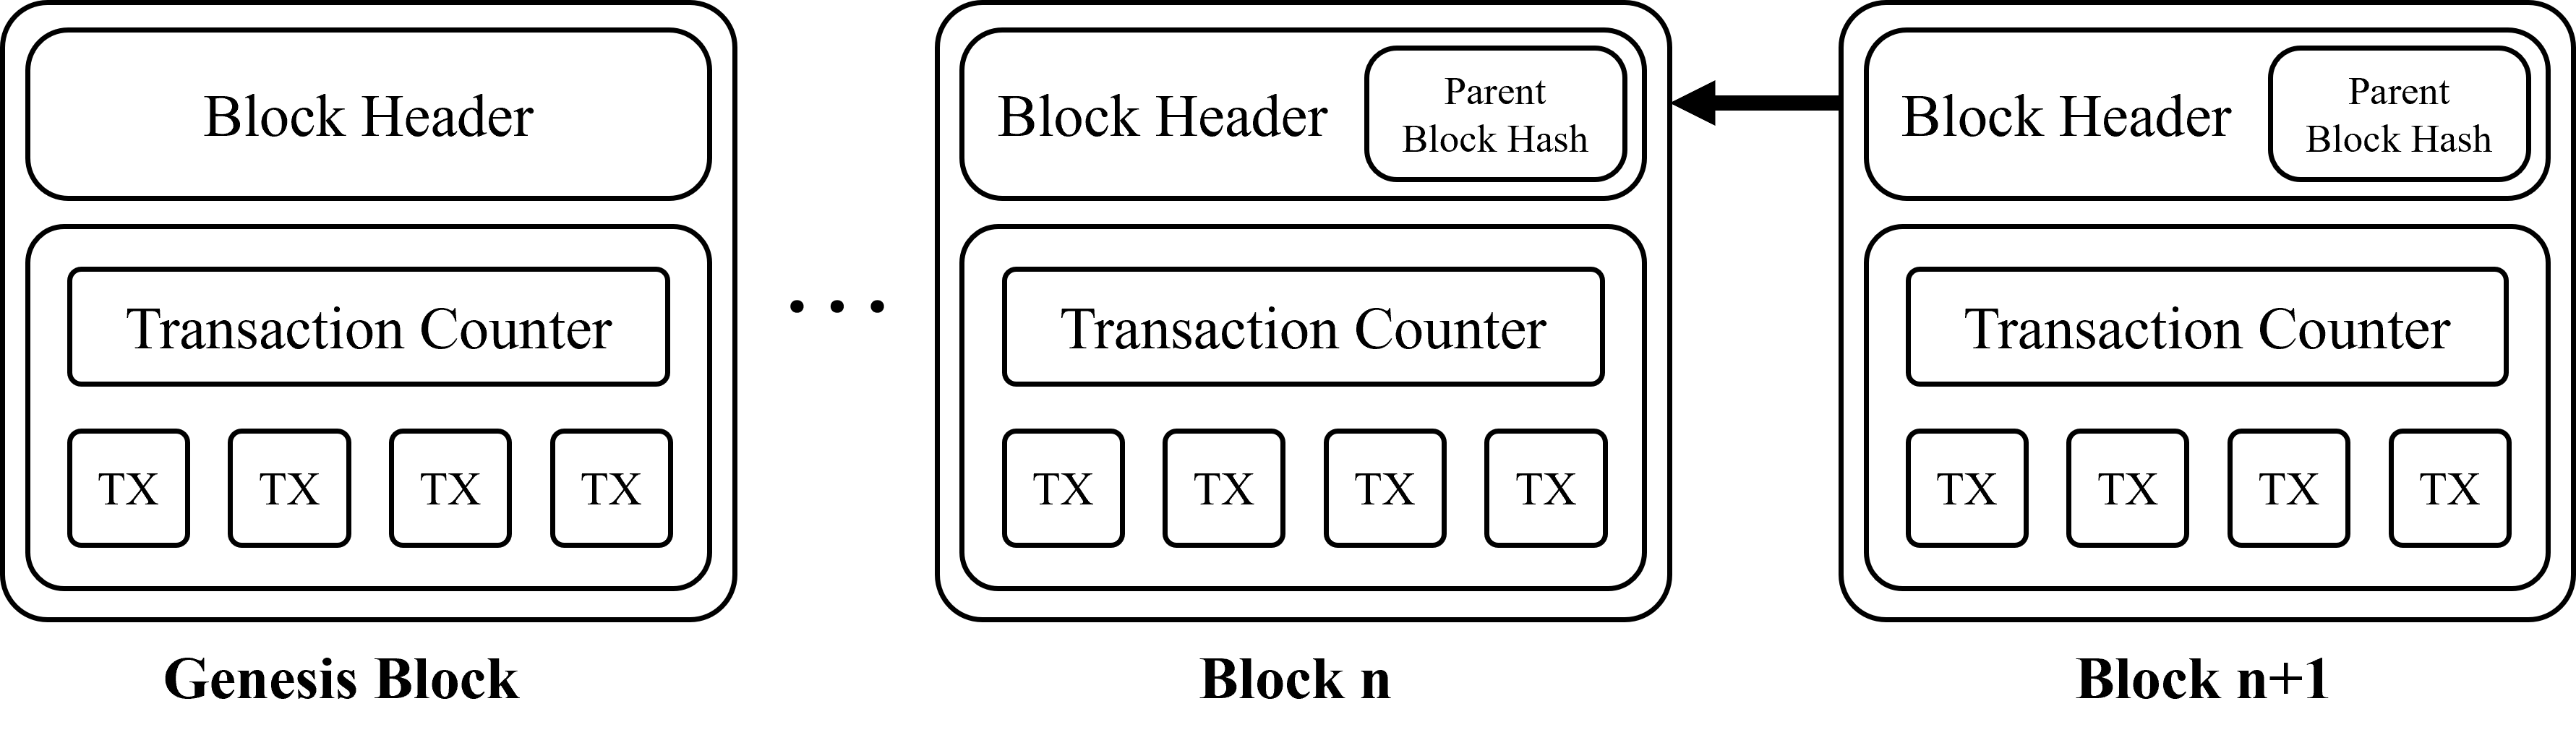
\includegraphics[width=0.8\linewidth]{figures/blockchain_block_structure.png}
    \caption{High-level block structure in blockchain.}
    \label{fig:blockchain_block_structure}
\end{figure}

\begin{figure}
    \centering
    
\includegraphics[width=0.85\linewidth]{figures/cryptocurrency_transaction_workflow.png}
    \caption{Cryptocurrency transaction workflow.}
    \label{fig:cryptocurrency_transaction_workflow}
\end{figure}

Figure \ref{fig:cryptocurrency_transaction_workflow} illustrates the involvement of the above components in a cryptocurrency transaction \cite{RN126}.

\section{Ethereum vs Bitcoin}

Bitcoin (BTC) is the first cryptocurrency that made use of blockchain technology; however, since its inception in 2008, the launch of Ethereum (ETH) in 2015 has been the next big milestone for cryptocurrencies \cite{palaiokrassas2023machine}. Unlike BTC, ETH is built as a more generalised application platform beyond just an exchange for digital currency \cite{RN138}. Ethereum has two key components \cite{RN138}:
\begin{itemize}
    \item Turing-complete virtual processor called Ethereum Virtual Machine (EVM) that allows for safe on-chain execution of smart contracts (code residing on the blocks which can be triggered if transactions meet a certain requirement).
    \item Ether, which is the currency of the network.
\end{itemize}

The first of the above two components is one of the differentiators of Ethereum in that Bitcoin does not have a Turing-complete processing capability \cite{RN138}. Furthermore, when a smart contract is executed on the blockchain, there is a micro-transaction fee associated with this computation, which is measured in the units called Gas \cite{RN138}. For every step of a smart contract that is executed, Gas is expended. Though these micro-transactions are inexpensive, exhaustive smart contracts can cause these fees to add up in the long run \cite{RN138}. As such, there is a limit imposed on the quantity of Gas that can be used per block, beyond which the users would be charged more to continue \cite{RN138}. By extension of the first component, when smart contracts (backend) are paired with a front-end user interface, the resulting product is called a Decentralised Application (DApp) \cite{RN138}. DApps have many real-world applications, such as in Decentralised Finance (DeFi), healthcare, copyright management, energy and many more \cite{palaiokrassas2023machine}.

Another key difference is the consensus used by the two coins. Bitcoin makes use of the PoW, where miners solve cryptographic puzzles (hash value), which is computationally expensive. The first miner that solves the puzzle adds the next block, along with receiving the block reward. Having this reward incentivises many miners to simultaneously solve the puzzle, resulting in extremely high energy consumption, which is not environmentally friendly. Originally, Ethereum (now known as Ethereum 1.0) employed PoW; however, to address the concerns of high power consumption, Ethereum 2.0 was rolled out in 2022 to make use of PoS. PoS involves a block proposer that compiles the transactions into a block and a set of validators to attest the block. These validators are chosen based on the amount of cryptocurrency they “stake”. The higher the stake, the higher the chance of being selected. A key advantage of PoS is that it reduces the block time significantly that leads to quicker confirmation of transactions. The problem with PoS is that it risks the centralisation of wealth, as the users with more Ether in their accounts get selected more often leading them to earn rewards more often.\cite{RN138}



% -----------------------------------------------------------------------------

\chapter{Related Work}
\label{chap:related_work}

This chapter reviews literature relevant to ETH price prediction, focusing on studies that explore the factors influencing ETH's value and the evolution of predictive modelling techniques. Particular attention is given to two foundational papers that are critically evaluated for their influence on the approach taken in this project. Rather than providing an exhaustive survey, the chapter focuses on influential works that guide the methodological direction of this research.

% methods for selecting meaningful input features,

\section{Factors Influencing Ethereum Prices}
Delfabbro \textit{et al.} \cite{delfabbro2021psychology} highlight that it is difficult to value cryptocurrencies when compared to stocks. This is because, unlike stocks, cryptocurrencies do not have traditional valuation anchors that depend on underlying assets, something that cryptocurrencies also lack \cite{bhatnagar2023demystifying}. At its core, the valuation is entirely on a speculative basis \cite{bhatnagar2023demystifying}. Therefore, it is important to understand the influential factors in conducting appropriate feature engineering for ML models.

Influential factors can be classified as internal and external factors \cite{poyser2019exploring} as shown in Figure \ref{fig:internal_external_factors} - an adaptation of \cite{khedr2021cryptocurrency}. Internal factors are primarily blockchain data, which can be seen as an alternative to metrics used in the fundamental analysis of stocks. On the other hand, external factors include capturing public perception, political aspects, and macroeconomics.  Although there are many factors, the key ones are price and volume, technical indicators, blockchain data, and public sentiment \cite{john2024cryptocurrency}. John \textit{et al.} \cite{john2024cryptocurrency} further states that of the four factors, the two that still require more research are technical indicators and blockchain data. However, the issue is that both cannot be explored together because blockchain data is difficult to source and is found mainly only at daily time intervals \cite{john2024cryptocurrency}, while technical indicators require data at a finer interval due to their use in day trading. As such, the perspective of this study was narrowed to use the remaining three to improve the studies done by Kim \textit{et al.} \cite{RN141} and Jagannath \textit{et al.} \cite{jagannath2021chain}. What follows in this section mainly stems from a critical review of the two studies, as summarised in Table \ref{tab:eth_price_comparison}.

\begin{figure}[tpbh]
    \centering
    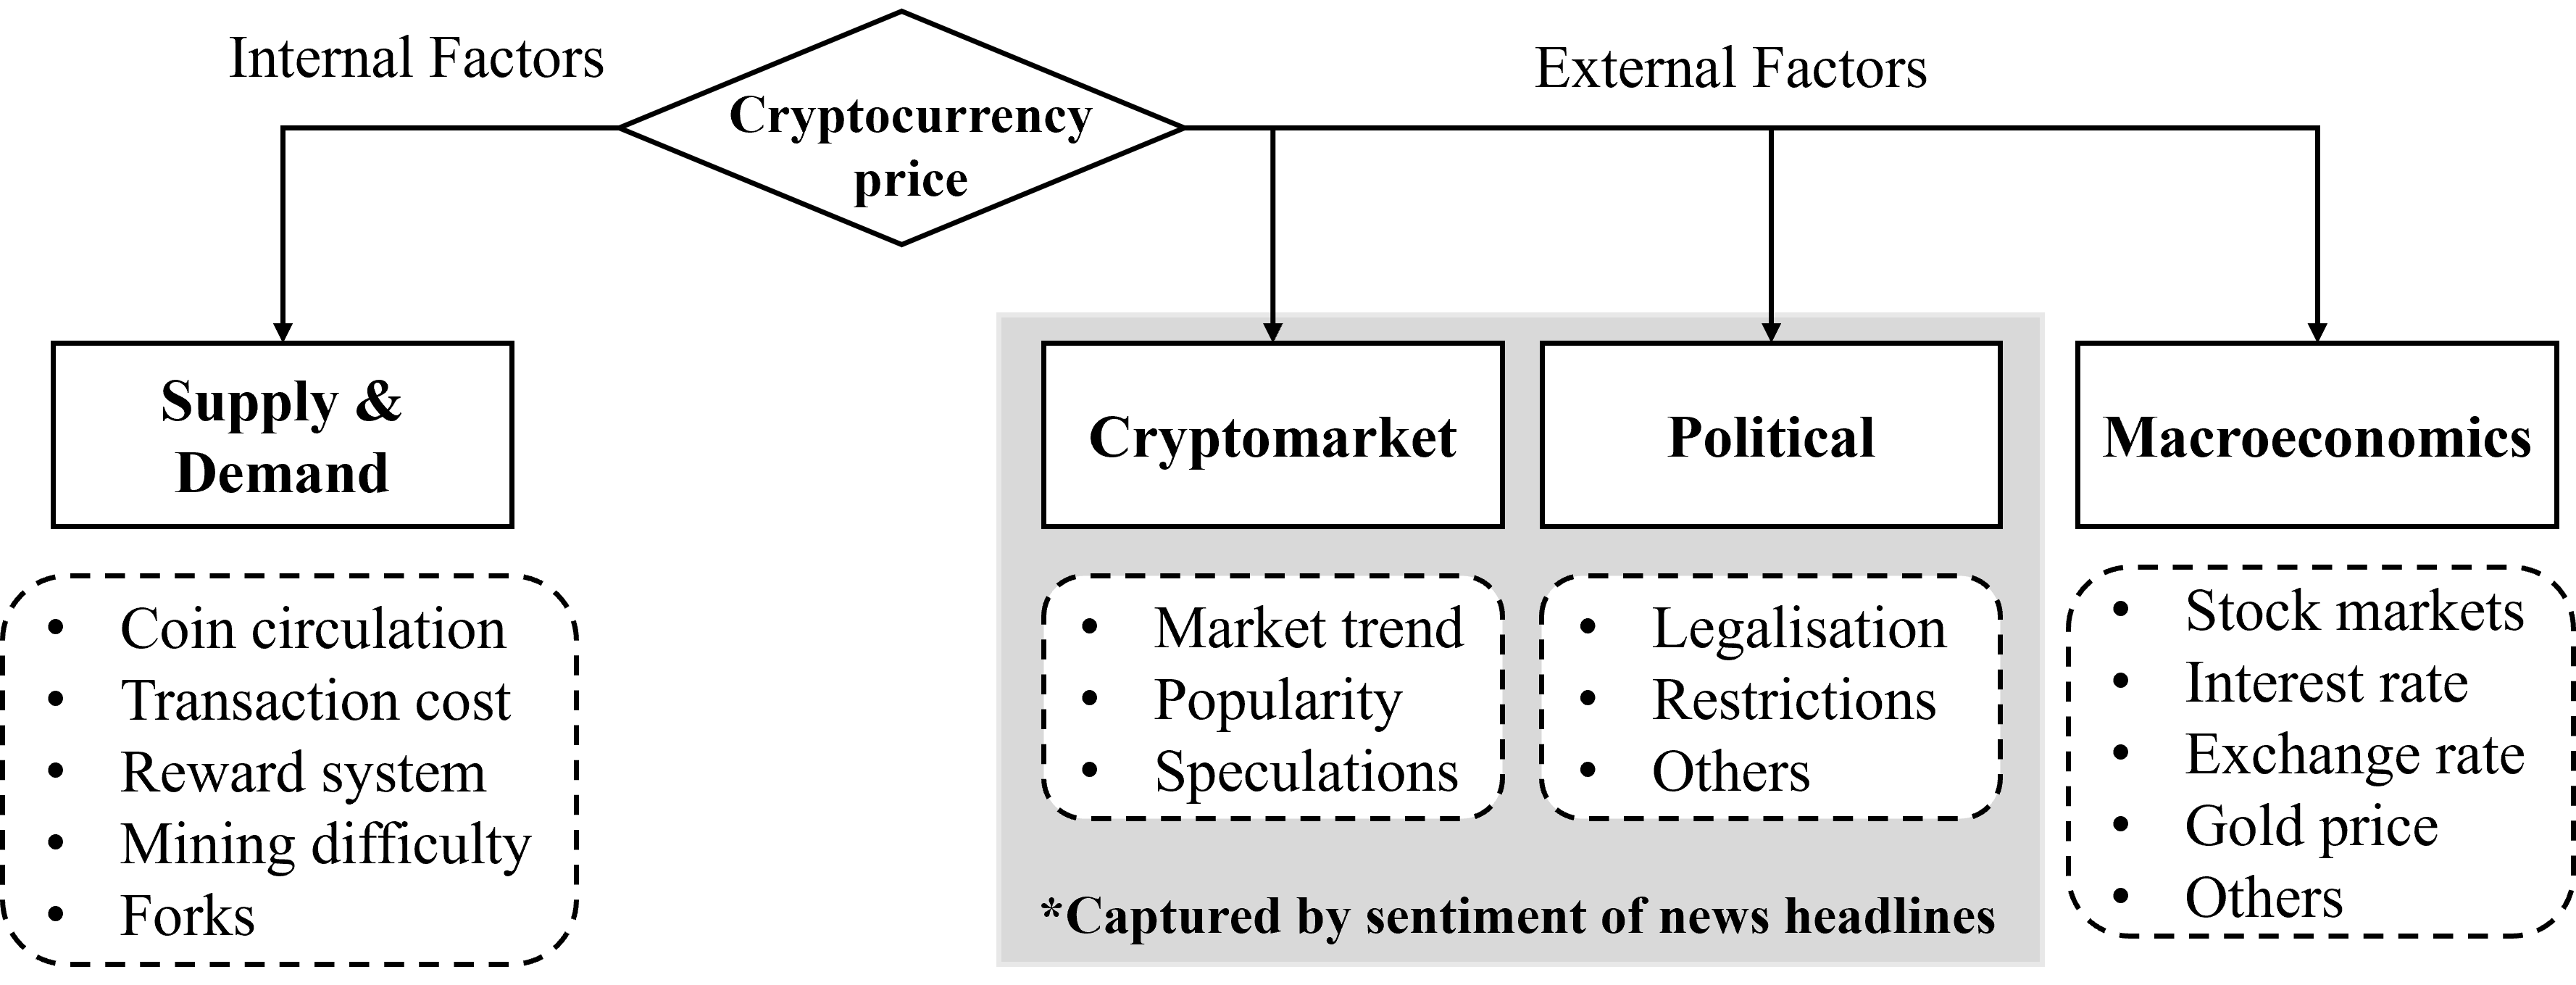
\includegraphics[width=0.9\linewidth]{figures/internal_external_factors.png}
    \caption{Segregation of internal and external factors influencing cryptocurrency price.}
    \label{fig:internal_external_factors}
\end{figure}

\newcolumntype{L}[1]{>{\RaggedRight\arraybackslash}p{#1}}

\begin{landscape}
\begin{table}[h]
\centering
\small
\caption{Summary of studies on ETH price prediction using blockchain data.}
\label{tab:eth_price_comparison}
\begin{tabular}{@{}L{3.5cm} L{5cm} L{4cm} L{4.5cm} L{5.5cm}@{}}
\toprule
\textbf{Study} & \textbf{Features} & \textbf{Models} & \textbf{Key Findings} & \textbf{Limitations} \\
\midrule

\textit{Predicting Ethereum prices with machine learning based on Blockchain information \cite{RN141}} & 
\begin{itemize}[leftmargin=*, nosep]
  \item 15 macroeconomic features
  \item 9 blockchain features for each BTC, LTC and DASH
  \item 8 generic blockchain features for ETH
  \item 4 ETH-specific blockchain features
\end{itemize}
& 
\begin{itemize}[leftmargin=*, nosep]
  \item Support Vector Machine (SVM)
  \item Artificial Neural Network (ANN)
\end{itemize}
& 
\begin{itemize}[leftmargin=*, nosep]
  \item ANN outperforms SVM
  \item Macroeconomic factors, ETH and BTC blockchain data improve performance
\end{itemize}
& 
\begin{itemize}[leftmargin=*, nosep]
  \item Use of some blockchain features irrelevant to Ethereum 2.0
  \item Lacks good baseline features
  \item No feature selection
  \item Next-day (implied) forecasts only
  \item Does not capture public sentiment
  \item No significance tests in results
  \item No explainability of models and their forecasts
  \item No baseline ML model
  \item Focuses only on regression metrics
\end{itemize} \\
\midrule

\textit{An On-Chain Analysis-Based Approach to Predict Ethereum Prices \cite{jagannath2021chain}} & 
\begin{itemize}[leftmargin=*, nosep]
    \item 26 ETH blockchain features
\end{itemize}
&
\begin{itemize}[leftmargin=*, nosep]
    \item Long Short-Term Memory (LSTM)
\end{itemize}
&
\begin{itemize}[leftmargin=*, nosep]
    \item L-SHADE optimisation algorithm yields the most accurate forecasts 
\end{itemize}
&
\begin{itemize}[leftmargin=*, nosep]
  \item Use of some blockchain features irrelevant to Ethereum 2.0
  \item No baseline features
  \item Basic feature selection using Pearson's and Spearman's correlation
  \item Next-day forecast only
  \item Does not capture public sentiment
  \item No significance tests in results
  \item No explainability of models and their forecasts
  \item Primary focus on optimisation algorithms for hyperparameter tuning rather than feature engineering
  \item Focuses only on regression metrics
\end{itemize} \\
\bottomrule
\end{tabular}
\end{table}
\end{landscape}

\subsection{Price and Volume}
Price and volume are easily available at various time intervals, albeit with limitations in the time range. Due to the commonality of these features, they have been heavily researched and proven to improve prediction in many studies. However, the recorded values for both features can differ depending on the data source.\cite{john2024cryptocurrency}

Kim \textit{et al.} \cite{RN141} explore a total of 54 features, where the effect was analysed by a step-wise addition of each categorical set as mentioned in Table \ref{tab:eth_price_comparison}. The problem with this method is that it lacks a feature selection step to identify feature importance, as it is unlikely that all features equally improve prediction. Moreover, the baseline features include 15 macroeconomic factors, which add unnecessary complexity and noise from the beginning. Here, a simpler set of features, including price and volume, would be beneficial. It is also important to note that Kim \textit{et al.} \cite{RN141} use ETH prices as a prediction target only and not also as a feature. Even adding days of the week as a categorical baseline feature is suitable, given that cryptocurrencies exhibit an intraweek seasonality pattern \cite{jasiak2024intraday}.

\subsection{Blockchain Data}
Blockchain data has been researched for price prediction significantly more for BTC than for any other coins \cite{john2024cryptocurrency,palaiokrassas2023machine}. Whilst inspiration can be drawn from those BTC studies to form hypotheses, it cannot be assumed that the same blockchain features will have the same level of effectiveness for other coins. This is because the blockchain data is unique to each coin, representing the health and activity of each network \cite{john2024cryptocurrency}. Therefore, feature selection is of the utmost importance.

The study done by Jagannath \textit{et al.} \cite{jagannath2021chain} explored 26 features in total, including price and volume. Although the study employs Pearson's and Spearman's correlation coefficients to conduct a basic feature selection, it fails to highlight the final set of blockchain features used in their models. Furthermore, the study does not have a stepwise addition of the final selected features; as such, there were no baseline features. This means there is no way to verify which blockchain features are effective if they are effective at all. Nevertheless, the study's primary focus was on investigating self-adaptive algorithms used in hyperparameter tuning of Long Short Term Memory (LSTM) deep learning (DL) model. As such, the relevance of this paper is less than that of Kim \textit{et al.} \cite{RN141}. 

One of the questions in Kim \textit{et al.}'s \cite{RN141} study examines the effectiveness of ETH-specific blockchain data, specifically uncle blocks, gas limits, gas prices, and gas consumption. Although the latter three are still relevant to ETH 2.0, uncle block is not. The concept of uncle blocks \footnote{An uncle block is a block that is mined almost the same time as another block, but is not added to the chain due to network latency; the miners would still be awarded partially for an uncle block \cite{RN141}.} is associated with PoW. Similarly, any other metrics associated with PoW, such as mining difficulty or hash rate (number of hash guesses per unit time), are irrelevant too. The novel contribution of Kim's study is that it also explores the effectiveness of blockchain data of highly correlated coins, including BTC, LTC and Dashcoin (DASH).

\subsection{Public Sentiment}
\label{sec:public_sentiment}

Both of the studies in Table \ref{tab:eth_price_comparison} do not make use of public sentiment as a feature. In general, public sentiment is captured using data from X (formerly known as Twitter) or Reddit social media posts \cite{john2024cryptocurrency}. Although X no longer supports free access to its public APIs \cite{john2024cryptocurrency}. Several studies highlighted in John et al.'s \cite{john2024cryptocurrency} survey prove that social media sentiment has been effective in predicting cryptocurrency prices. But a key challenge that remains is to filter out the noise, sarcasm or even misinformation \cite{john2024cryptocurrency}.

Alternatively, public sentiment can also be speculated through the analysis of news headlines. The benefit of using news headlines over social media is that it is more credible, if sourced correctly, and can collectively capture both political news and associated sentiment. A presumptive limitation of using news headlines is that it could fail to capture the speculative nature of cryptocurrencies \cite{john2024cryptocurrency}. This is because news headlines provide no information on the public's network effect. Not knowing the reach of the information (views) or how the audience has reacted (likes and comments) to the news can mean the difference between being an effective source and not. Nevertheless, studies \cite{anamika2022news}, \cite{RN146} and \cite{bhatnagar2023demystifying} claim that news headline sentiment does affect price/volatility.

Identifying the source solves one-half of the problem; conducting the sentiment analysis is the remaining half. There are several ways to conduct sentiment analysis, but at a granular level, the approaches can be classified as lexicon-based, ML-based, DL-based, transformer-based and hybrid \cite{kumar2025evolving}. At a higher level, they can be categorised into supervised and unsupervised methods. Given the difficulty of acquiring a labelled dataset large enough to train and test \cite{araci2019finbert}, unsupervised methods would be relevant and preferred. Therefore, the key methods to focus narrow down to lexicon-based and transformer-based approaches. The benefits of lexicon-based approaches are that they are simple, easy to explain and ideal for short texts \cite{birjali2021comprehensive}. However, general-purpose lexicons struggle with domain-specific languages and also lack contextual understanding \cite{birjali2021comprehensive}. This is where transformer-based approaches excel. Transformers use a deep neural network (DNN) architecture along with a self-attention mechanism to understand contextual nuances in longer pieces of text \cite{kumar2025evolving}. Moreover, pre-trained transformers that are fine-tuned to a specific domain can make them more accurate in sentiment analysis \cite{kumar2025evolving}. Similar to DNNs, transformers also act as a black box for interpretability and have a high computational cost.

\section{Forecasting Models}
At its core, forecasting prices of cryptocurrencies is a time-series problem. The challenge lies in the fact that many real-world time series exhibit non-stationarity and/or non-normality \cite{hewamalage2023forecast}. Non-stationary time series typically includes attributes such as seasonality,  heteroscedasticity\footnote{Change of variance over time (i.e. checks if volatility changes over time or not).} and structural breaks\footnote{A sudden change in the time series which could be due to a change in any combination of mean, variance and trend.} \cite{hewamalage2023forecast}. Non-normality includes non-symmetric distributions, usually with high occurrences of extreme values \cite{hewamalage2023forecast}. Both make it difficult to accurately forecast prices using traditional statistical approaches that are dependent on normality and stationarity. As a result, ML models that do not make these assumptions and can learn complex non-linear patterns are beneficial. Predicting prices is a regression problem; however, in the context of generating profits, the price direction (up/down) is sufficient and, as such, can also be a binary classification problem. What follows is a review of the evolution of methods used in forecasting. Given that ETH is not as heavily researched, BTC studies are also used where required to form a case in point. The inner workings of the models experimented with in this study are explained further in Chapter \ref{chap:methodology}.

\subsection{Statistical Models}
\label{sec:statistical_models}
A common statistical model used in time-series forecasting studies is the autoregressive integrated moving average (ARIMA) \cite{sailaja2024crypto}. This is because it is one of the simplest models that can handle unit-root\footnote{A property of non-stationarity capturing stochastic trends resulting from shocks that have a permanent effect over time.} non-stationarity and serves as a good baseline model. It is essential to note that ARIMA is a valid baseline only if the forecasts extend beyond one step forward, albeit still for short-term predictions. A more appropriate baseline for one-step forward forecasting would be a Naive forecast, where the best guess for the next value is the last known value. The documentation of common pitfalls in time-series forecasting by Hewamalage \textit{et al.} \cite{hewamalage2023forecast} demonstrates that even Naive forecasts can outperform ML models for a one-step forward forecast. To use ARIMA for long-term forecasting, it is a common practice to refit the model as new data becomes available \cite{hewamalage2023forecast}, also known as a walk-forward approach. Although ARIMA does not include the seasonality (S) or exogenous (X) components, it is possible to incorporate these components in its counterparts, such as SARIMA, ARIMAX, or even a combination, SARIMAX.

\subsection{Machine Learning Models}
ML models used for time series have evolved from traditional methods such as linear regression, SVM, Naive Bayes, to methods such as Random Forests (RF) or Extreme Gradient Boosting (XGBoost), incorporating ensemble techniques like bagging and boosting, respectively \cite{john2024cryptocurrency}. However, since the introduction of DL methods, hybrid DL methods have also been experimented with \cite{john2024cryptocurrency}. Whilst transformers are currently regarded as state-of-the-art, they still require more research, and will not be looked at in this study \cite{john2024cryptocurrency}. This is because the primary focus of this study is on feature engineering; ensemble, DL and hybrid DL already cover the established model spectrum to make Kim \textit{et al.}'s \cite{RN141} study relevant before proceeding to the state-of-the-art. 

\subsubsection{Ensemble}
Light Gradient Boosting Machine (LightGBM), XGBoost, Adaptive Boosting (AdaBoost) and Categorical Boosting (CatBoost) have all been previously used for cryptocurrency price forecasting, and are considered state-of-the-art Gradient Boosting Machines (GBMs) \cite{bouteska2024cryptocurrency,de2023practical, sun2024cryptocurrency}. Given that ensemble methods make use of multiple models (trees), they allow for better generalisation, along with being able to learn complex non-linear patterns. These benefits come with an increased computational cost compared to traditional ML models, though less than that compared to DL models. Studies \cite{bouteska2024cryptocurrency}, \cite{de2023practical} and \cite{ sun2024cryptocurrency} demonstrate that ensemble methods can not only outperform traditional methods, but also DL methods such as LSTM, which are specific to time series. Whilst Bouteska \textit{et al.} \cite{bouteska2024cryptocurrency} show that LightGBM is the best ensemble technique, it does not include the use of XGBoost. Studies done by Sun \cite{sun2024cryptocurrency} and De Rosa \textit{et al.} \cite{de2023practical} do include this comparison, and show that XGBoost outperforms LightGBM. 

\subsubsection{Deep Learning}

ANN is one of the simplest of the DL models and was implemented by Kim \textit{et al.} \cite{RN141}. The choice of using this method was justified by Kim due to its ability to handle non-linear patterns across various domains such as financial analysis, natural language processing (NLP), image recognition, and more \cite{RN141}. However, Recurrent Neural Network (RNN) type DL models are more suited to handling temporal dependencies and sequential data because of their ability to remember previous input \cite{mazinani2025deep}. There are three different types of RNNs: simple RNN, LSTM and Gated Recurrent Unit (GRU). While simple RNNs are lightweight and suitable for short-term sequences, they struggle with a phenomenon known as the vanishing gradient problem \cite{mazinani2025deep}. This is when gradients (learning signal) become rapidly smaller as they pass through time steps and layers, making it harder for the model to learn until it eventually stops. This problem is resolved in both the LSTM and GRU architectures \cite{mazinani2025deep}. Generally, LSTM can remember long-term dependencies better than GRU due to a dedicated memory cell, but it is more computationally expensive, as shown in \cite{hansun2022multivariate}. Regardless of this generalisation, studies \cite{hansun2022multivariate}, \cite{seabe2023forecasting} and \cite{hamayel2021novel} show that the best performing architecture can be either depending on the coin, time frame, and lags analysed. Studies \cite{mazinani2025deep}, \cite{hansun2022multivariate}, and \cite{seabe2023forecasting} also demonstrate that the bidirectional versions of both (BiLSTM and BiGRU) typically have improved performance compared to their unidirectional counterparts, since they pass the sequence in reverse to identify more patterns.

\subsubsection{Hybrid Deep Learning}
Convolutional Neural Networks (CNN) have also been used for time series, though it is more common in imaging-based applications \cite{mazinani2025deep}. At a high level, CNNs can identify and capture local patterns (seasonality, change in trends, etc.). Moreover, it is much faster than RNNs but cannot remember complex long-term dependencies. However, when these benefits are paired with an RNN type, the resulting hybrid DL model can outperform both RNNs and CNNs, as shown by the study \cite{mazinani2025deep}. As such, the core idea behind hybrid DL models is that the advantages of one architecture counteract the limitations of another \cite{john2024cryptocurrency}. However, due to their complex architectures, hyperparameter tuning is challenging and also has a high computational cost \cite{john2024cryptocurrency}. CNN-RNN hybrid models are common in the space of cryptocurrency price prediction and have proven their efficacy in several studies \cite{mazinani2025deep, RN97, yu2024comparative, kang2022cryptocurrency, hoa2025hybrid}.

% \subsection{Feature selection methods}
% granger causality test
% feature importance
% mutual information
% - blockchain features (1 study at best but limited to, with higher focus on bitcoin and no clear features selection) \footnote{test}
% - sentiment analysis (comparison of models, resulting in best predictive sentimetn scores)
% - 7 day forecasting 
% + explainable AI

% -----------------------------------------------------------------------------
\chapter{Data}
\label{chap:data}
This chapter presents a comprehensive overview of the data used in this study. It outlines the sources from which the data were obtained, the specific features extracted from each source, and the rationale for their inclusion. The chapter also includes a comparative analysis of the compiled dataset against the benchmark study by Kim \textit{et al.} \cite{RN141}, highlighting similarities and differences in data selection. Furthermore, this chapter conducts an exploratory data analysis (EDA) to uncover patterns, trends, and potential anomalies in the data. These insights serve as supporting evidence for the design choices and preprocessing strategies discussed in the subsequent chapter. The goal is to ensure that the model development is grounded in a deep understanding of the underlying data landscape.

\section{Sources}
The primary criterion for acquiring all the data was that it had to be open-source to ensure the study's reproducibility. At the time of writing this dissertation, only one of the sources is no longer open-source; however, this will be explained further in the subsections below. Subsidiary criteria included that the most recent data should be as complete as possible to ensure the reliability and the relevancy of the work; as such, different features were extracted from different sources, though cross-compared where possible to check for similarity. 

\subsection{Price and Volume}
ETH price and volume were sourced from Yahoo Finance (YF), along with the same for BTC and LTC. The reason for including BTC and LTC is that they are two of the most highly correlated cryptocurrencies \cite{seabe2023forecasting, hamayel2021novel}.
The data acquired from YF include the opening, high, low, closing (OHLC) and adjusted closing prices, along with the volume at daily intervals. Adjusted closing prices for cryptocurrencies are the same as the closing price, as they do not include events such as dividends, stock splits, and rights offerings that are typical of stock markets. Moreover, the closing price of the stock market is commonly used as the prediction target in ML tasks, and the same is also acceptable for cryptocurrencies. However, a problem with using closing prices is that different cryptocurrency exchanges report different closing prices. Furthermore, since cryptocurrency can be traded 24/7, its closing price is not a true representation of the entire day. To account for these differences, the average price of OHLC was used as the prediction target.

\subsection{Blockchain Data}
To address the aim of this study, the acquisition of blockchain data was crucial. This was done using three separate sources: Etherscan (ES), OkLink (OL) and BitInfoCharts (BIC). The data from ES and OL were downloaded directly as Comma Separated Values (CSV) files from the dashboard graphs, though OL no longer allows a direct download and is no longer open-source. The data from BIC was scraped from its website. Whilst OL and BIC contained data for ETH, BTC and LTC, ES only had data for ETH. All the features collected are at a daily time interval and summarised in Table \ref{tab:blockchain_features}. The table shows if each feature is an indicator of supply and/or demand of the coins, and also a comparison to the features included in \cite{RN141}. As seen in the table, Block Count and Generated Coins were the only two features which could not be sourced for all coins. For BTC and LTC, Average Block Time and On-chain Transaction Volume were the additional features that could not be sourced. Here, the introduction of on-chain and off-chain transactions is important as it is a concept that was not explained in the previous chapters. Transactions recorded on the blockchain are considered on-chain and are in line with the core principles of cryptocurrencies. However, transactions can occur off the chain as well, and this is typical of CEX to increase the speed of transactions whilst also having lower transaction fees \cite{barbon2021quality}. Since these values still reflect usage of the cryptocurrency, and therefore its demand, it was deemed important to include these features as well. Another key point to highlight from Table \ref{tab:blockchain_features} is the addition of five extra features that are not used in \cite{RN141}.

\begin{table}[H]
\centering
\caption{Summary of features collected for each coin and their hypothesised indicator.}
\label{tab:blockchain_features}
\begin{adjustbox}{max width=\textwidth}
\begin{threeparttable}
\begin{tabular}{p{4cm} p{4cm} c c c c c}
\toprule
\textbf{\raggedright Feature (Units)} & \textbf{Definition} & \textbf{Indicator} & \textbf{Used in \cite{RN141}?} & \multicolumn{3}{c}{\textbf{Source}} \\
\cmidrule(lr){5-7}
 & & & & \textbf{ETH} & \textbf{BTC} & \textbf{LTC} \\
\midrule
% Sample rows
\raggedright Average Price (USD) & \raggedright Average of OHLC prices & - & \ding{51} & YF & YF & YF \\
\raggedright Total Volume & \raggedright No. of coins traded on and off-chain & Demand & \ding{51} & YF & YF & YF \\
\raggedright On-chain Transaction Count & \raggedright No. of transactions completed on-chain & Demand & \ding{51} & OL & OL & OL \\
\raggedright Average Transaction Fees (USD) & \raggedright Average fee to complete a transaction & Demand & \ding{51} & ES & OL & OL \\
\raggedright Active Addresses & \raggedright No. of wallet addresses that have sent and/or received a transaction & Demand & \ding{51} & ES & OL & OL \\
\raggedright Average Block Size (kB) & \raggedright Average memory of blocks created & Demand & \ding{51} & ES & OL & OL \\
\raggedright Block Count & \raggedright No. of blocks created & Demand & \ding{51} & \ding{55} & \ding{55} & \ding{55} \\
\raggedright Difficulty$^{\text{†}}$ & \raggedright Difficulty in creating a block & Supply & \ding{51} & \ding{55} & OL & OL \\
\raggedright Average Block Time (s) & \raggedright Average time to create and add a block to the chain & Supply & \ding{51} & ES & \ding{55} & \ding{55} \\
\raggedright Generated Coins & \raggedright No. of coins issued & Supply & \ding{51} & \ding{55} & \ding{55} & \ding{55} \\
\raggedright Gas Limit* & \raggedright Amount of gas allowed per block & - & \ding{51} & ES & \ding{55} & \ding{55} \\
\raggedright Gas Used*  & \raggedright Total gas used & Demand & \ding{51} & ES & \ding{55} & \ding{55} \\
\raggedright Average Gas Price* (GWei) & \raggedright Average price per unit gas to enter information into the block & Demand & \ding{51} & ES & \ding{55} & \ding{55} \\
\raggedright Deployed Contracts* & \raggedright No. of smart contracts published on the blockchain & Demand & \ding{55} & ES & \ding{55} & \ding{55} \\
\raggedright Verified Contracts* & No. of smart contracts that have a public source code which matches on-chain code & Demand & \ding{55} & ES & \ding{55} & \ding{55}\\
\raggedright New Addresses &\raggedright No. of wallet addresses appearing first time on the blockchain & Demand & \ding{55} & OL & OL & OL \\
\raggedright On-chain Transaction Volume & \raggedright No. of coins traded on-chain only & Demand & \ding{55} & OL & OL & \ding{55} \\
\raggedright Hash Rate$^{\text{†}}$ (Hash/s) & \raggedright No. of hashes performed per second by miners & Supply & \ding{55} & \ding{55} & BIC & BIC \\
% Add more rows as needed
\bottomrule
\end{tabular}
\vspace{0.5em}
\begin{tablenotes}
\footnotesize
\item[†] Features not applicable to ETH 2.0.
\item[*] ETH-specific blockchain data.
\end{tablenotes}
\end{threeparttable}
\end{adjustbox}
\end{table}

\subsection{News Headlines}
\texttt{GNews} \cite{Abdullah2024}, a Python library, was used to fetch daily news headlines from Google News. As part of the API calls made by the library, the keywords that were used to filter the relevant headlines were: `Cryptocurrency', `Blockchain', `Ethereum', `Bitcoin' and `Litecoin'. The data fetched included the news headlines, the website link of the article, description (duplication of the news headline) and the publisher.

\section{Exploratory Data Analysis (EDA)}
\label{sec:eda}
Given the large number of features, the aim of this EDA was not to be exhaustive but rather twofold:
\begin{itemize}
    \item To select an appropriate range of dates used for machine learning.
    \item Key insights about the target and features that help with the explainability of ML models.
\end{itemize}

The date range of all raw data was dictated by the start and end dates of the ETH price data obtained from YF, which were 09/11/2017 and 10/08/2024, respectively. However, certain features had a significant continuous portion of missing data, which could not be interpolated, thus limiting the usable data. Table \ref{tab:missing_features} below summarises the proportion of the entire date range that is missing and the usable date range. It is evident, ETH and BTC have more complete data, and LTC is the main restrictor.

\newcolumntype{C}[1]{>{\centering\arraybackslash}p{#1}}
\begin{table}[H]
\centering
\caption{Summary of missing data.}
\label{tab:missing_features}
\begin{adjustbox}{max width=\textwidth}
\begin{tabular}{p{5cm} C{1.25cm} C{1.25cm} C{1.25cm} c}
\toprule
\textbf{\raggedright Feature} & \multicolumn{3}{c}{\textbf{Missing Proportion (\%)}} & \textbf{Usable Date Range}\\
\cmidrule(lr){2-4}
 & \textbf{ETH} & \textbf{BTC} & \textbf{LTC}  &\\
\midrule
% Sample rows
\raggedright Average Price & 0& 0& 0 & Maximum \\
\raggedright Total Volume & 0 & 0& 0& Maximum \\
\raggedright On-chain Transaction Count & 0& 0& 5.55 & 09/11/2017 - 01/04/2024 \\
\raggedright Average Transaction Fees & 0 & 0& 5.55& 09/11/2017 - 01/04/2024 \\
\raggedright Active Addresses & 0& 0.04& 0.04 & Maximum \\
\raggedright Average Block Size & 0& 0& 5.55 & 09/11/2017 - 01/04/2024 \\
\raggedright Difficulty & - & 0& 5.55 & 09/11/2017 - 01/04/2024 \\
\raggedright Average Block Time & 0& -& - & Maximum \\
\raggedright Gas Limit & 0& -& - & Maximum \\
\raggedright Gas Used  & 0& -& - & Maximum \\
\raggedright Average Gas Price & 0& -& - & Maximum \\
\raggedright Deployed Contracts & 0& -& - & Maximum \\
\raggedright Verified Contracts & 0& -& - & Maximum\\
\raggedright New Addresses &1.82& 0& 5.55 & 09/11/2017 - 01/04/2024 \\
\raggedright On-chain Transaction Volume & 1.13& 0& - & Maximum \\
\raggedright Hashrate & - & 0& 0& Maximum\\
% Add more rows as needed
\bottomrule
\end{tabular}
\end{adjustbox}
\end{table}

The second aspect that helped to select the date range was a deeper analysis of the new headlines. From the above analysis, it is clear that the usable date range was between 09/11/2017 and 01/04/2024. In that date range, a total of 134135 headlines were collected from 7223 unique publishers. The top 20 publishers accounted for approximately 36\% of all headlines as summarised in Figure \ref{fig:top_20_publishers}.

\begin{figure}[H]
    \centering
    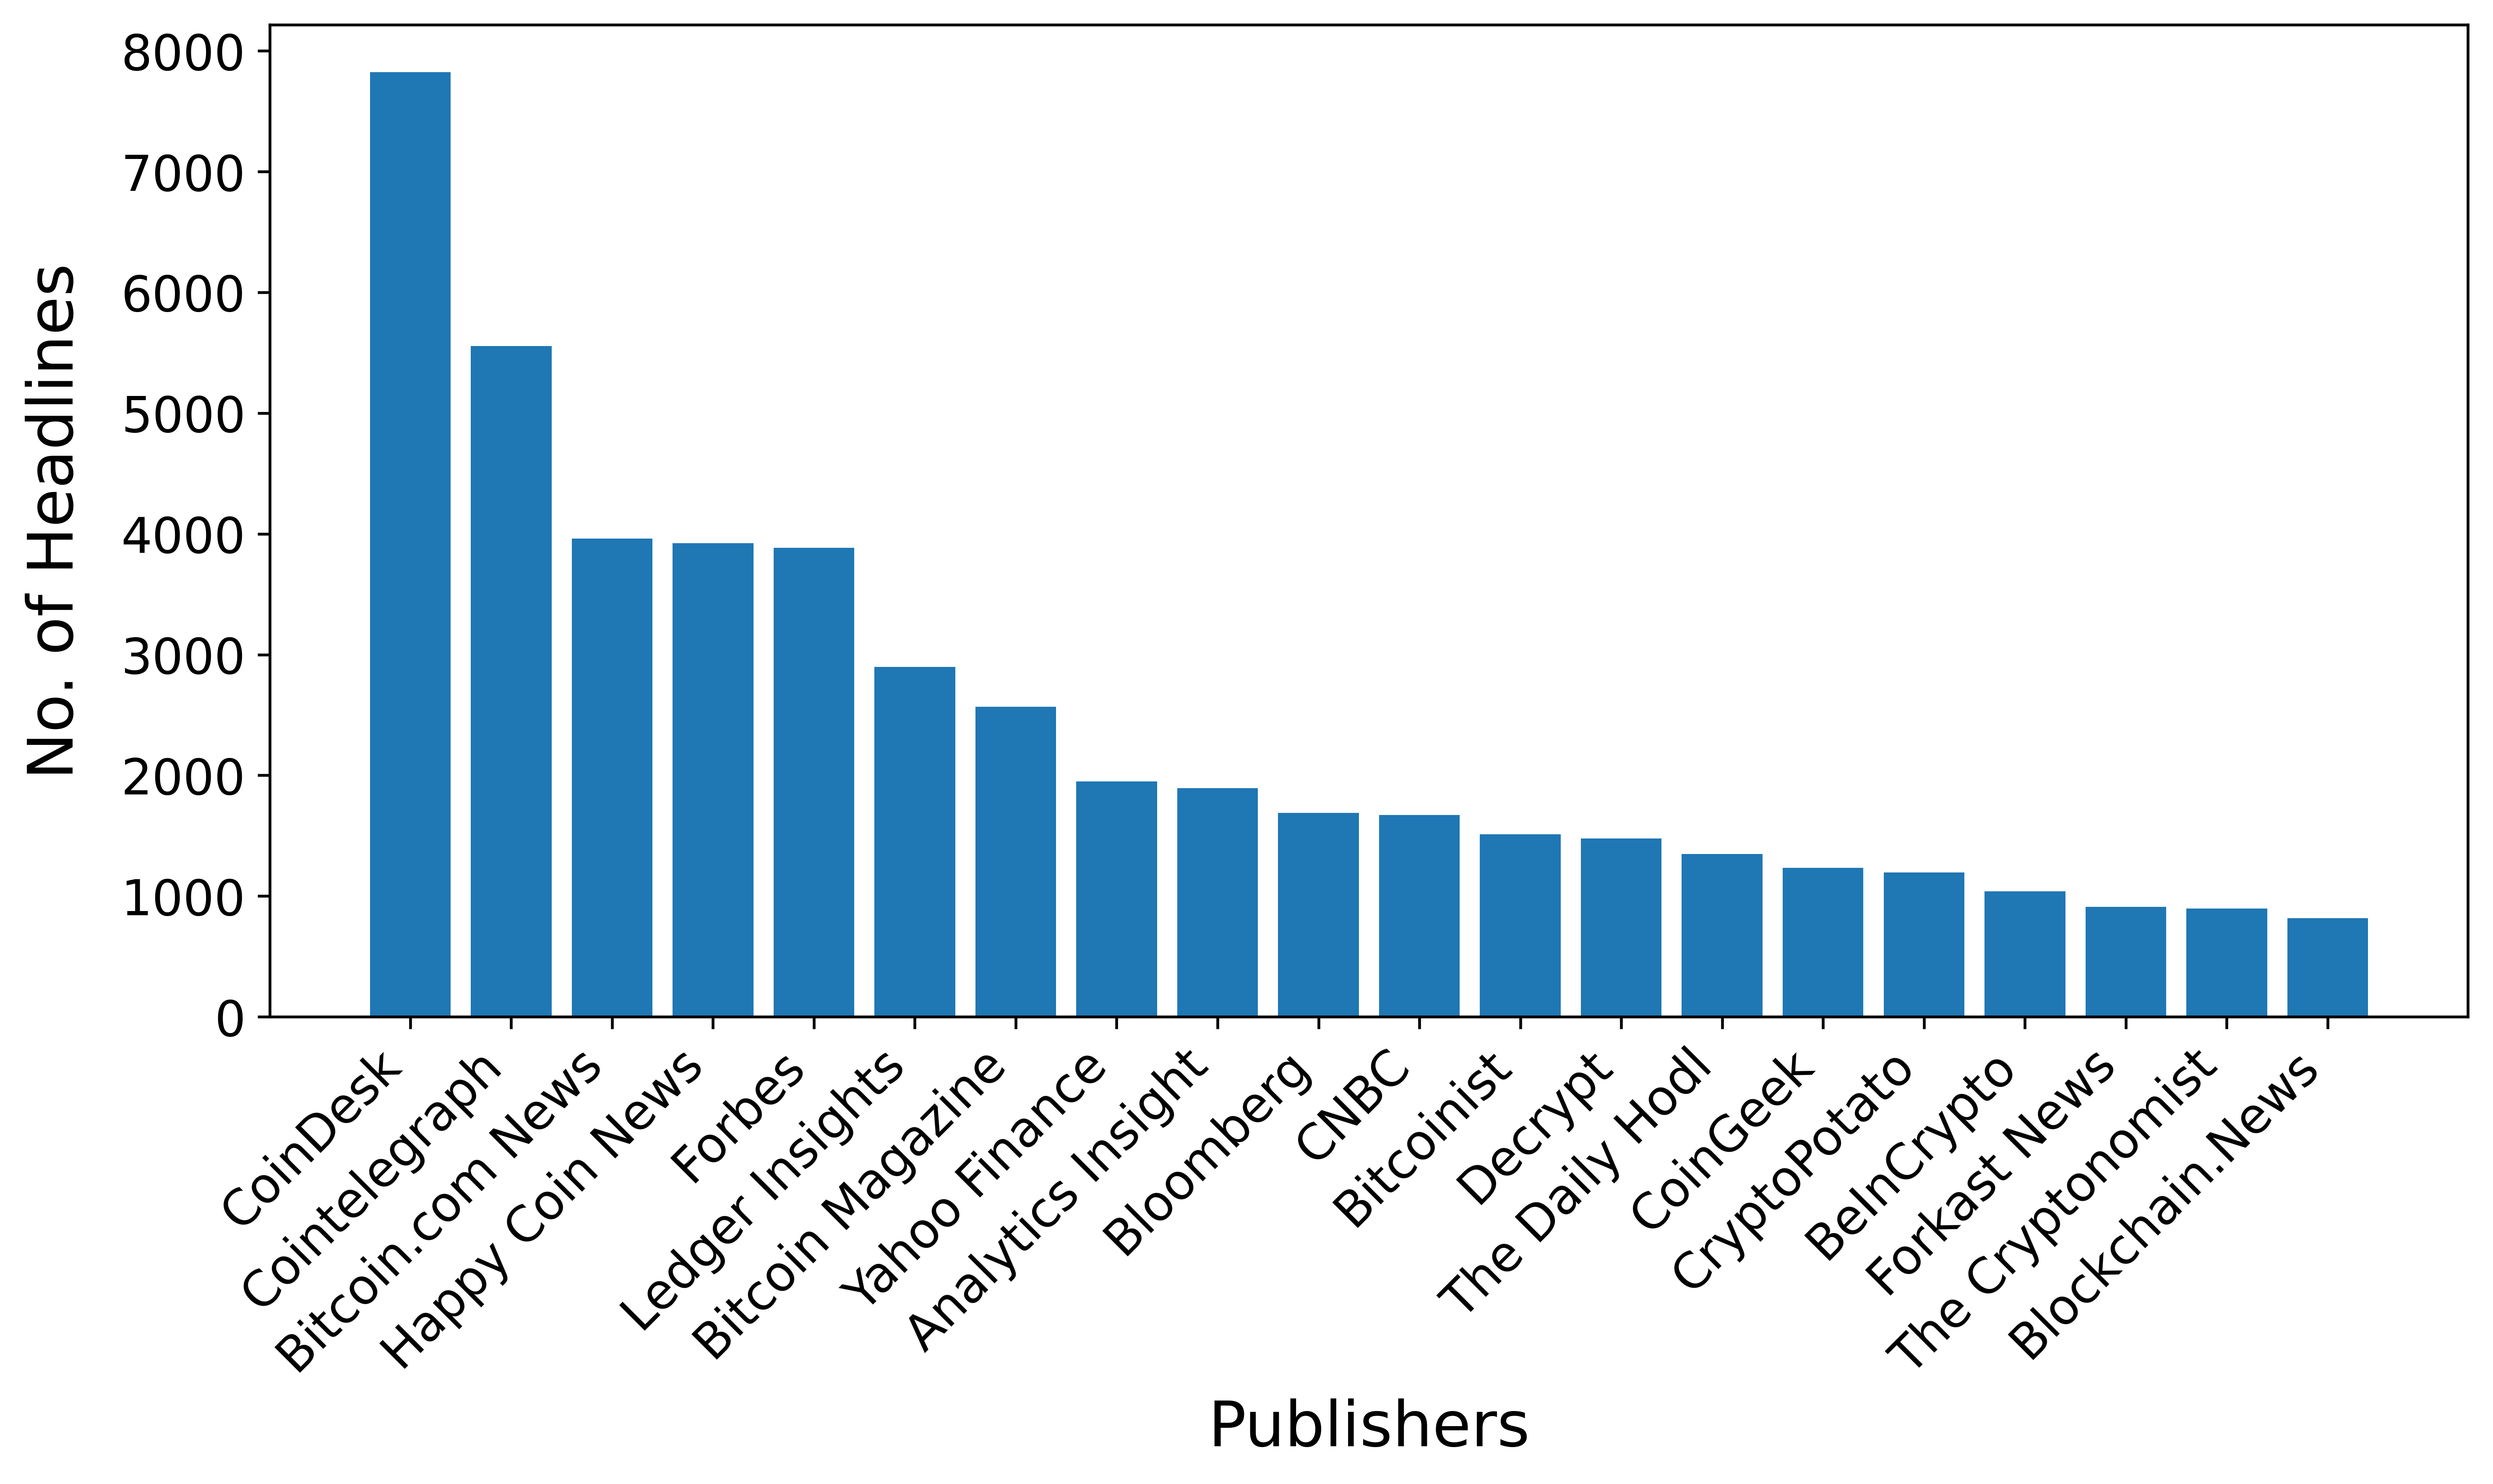
\includegraphics[width=0.8\linewidth]{figures/top_20_publishers.png}
    \caption{Top 20 publishers of the news headlines collected.}
    \label{fig:top_20_publishers}
\end{figure}

At a granular level, Figure \ref{fig:headline_frequency_distribution} shows a higher volume of headlines collected for more recent years, with a distinct sharp increase in the average number of daily headlines between 2020 and 2021, and 2023 and 2024. An increase in the number of headlines is expected over the years due to improved data availability and increased media coverage. However, an abrupt change in the volume of headlines can introduce a bias in the sentiment trend, where the ML model may interpret recent times as more volatile. To avoid this situation, data from 01/01/2021 to 31/12/2023 would be a safe choice. Another key observation from Figure \ref{fig:headline_frequency_distribution} is that the distribution is about even across the months for each year.

\begin{figure}[H]
    \centering
    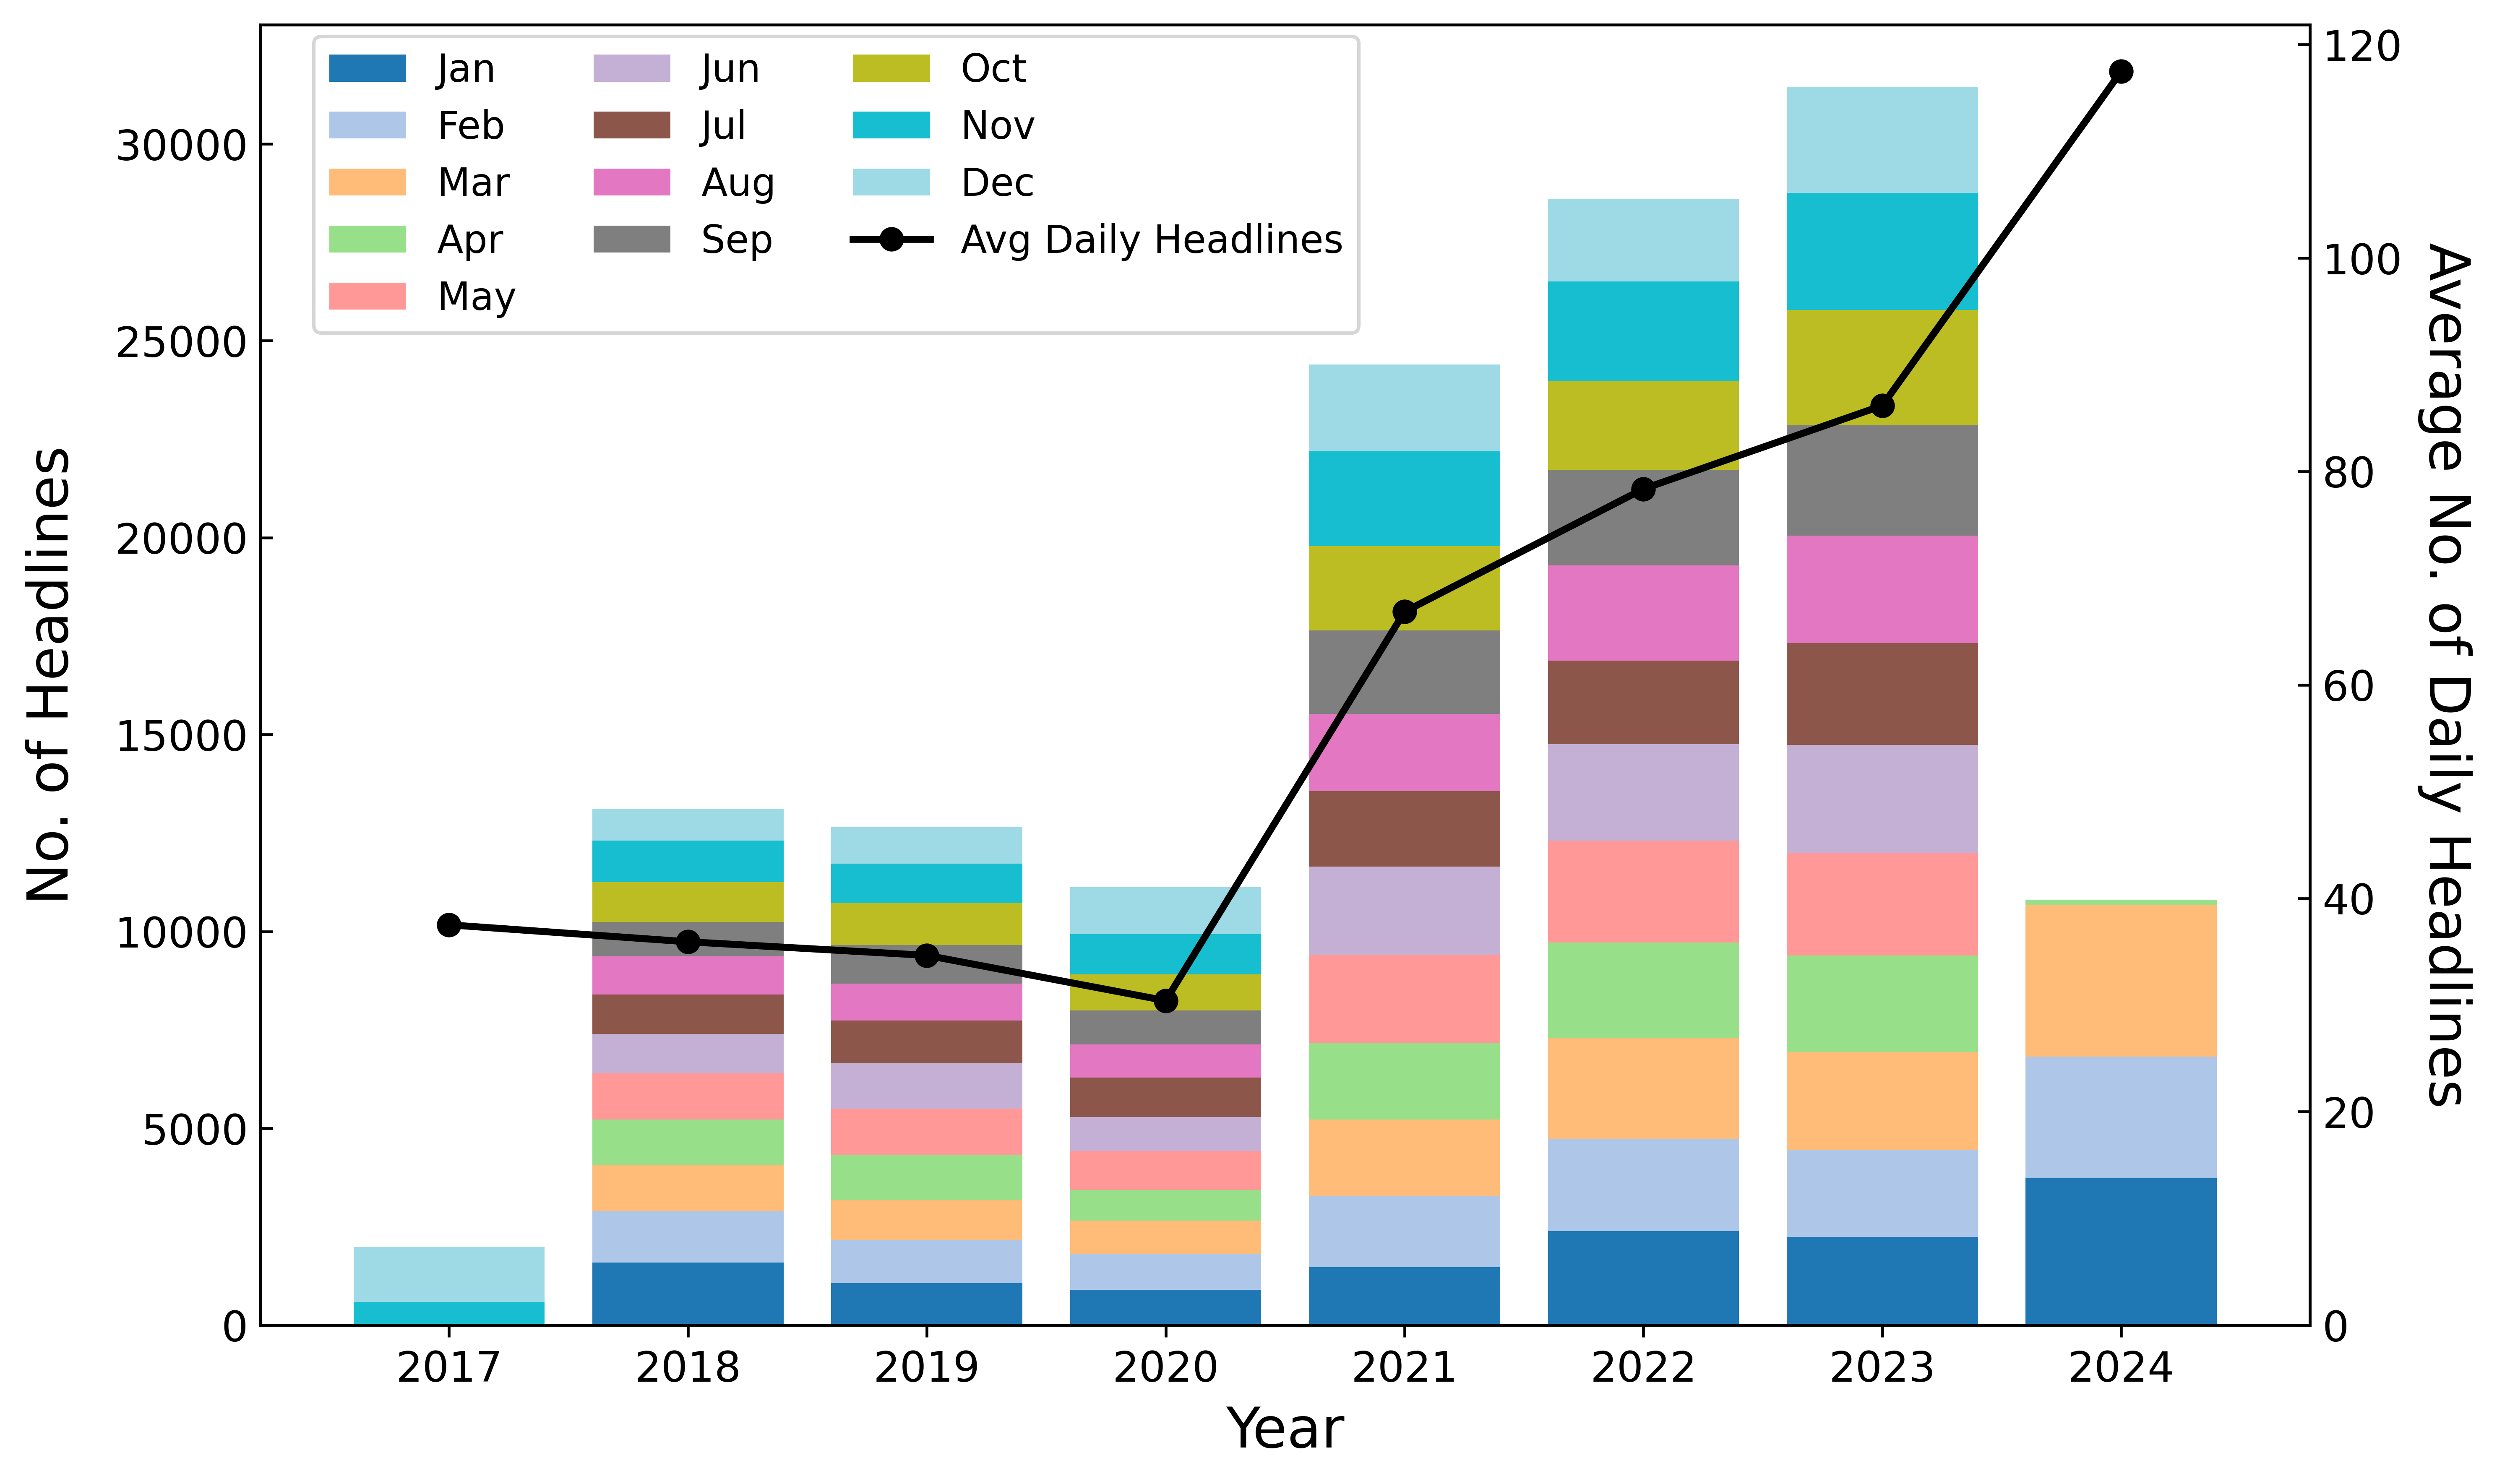
\includegraphics[width=0.8\linewidth]{figures/headline_frequency_distribution.png}
    \caption{No. of headlines aggregated at daily, monthly and yearly intervals.}
    \label{fig:headline_frequency_distribution}
\end{figure}

The final selected date range consists of 84,451 headlines from 5,657 unique publishers, with all days having at least 1 or more headline. Moreover, the distribution of the headline length is only slightly positively skewed (Figure \ref{fig:headline_length_distribution}), mainly due to some unusually long headlines as depicted by the maximum value. As part of pre-processing, these longer headlines need to be filtered out based on their legitimacy.

\begin{figure}[H]
    \centering
    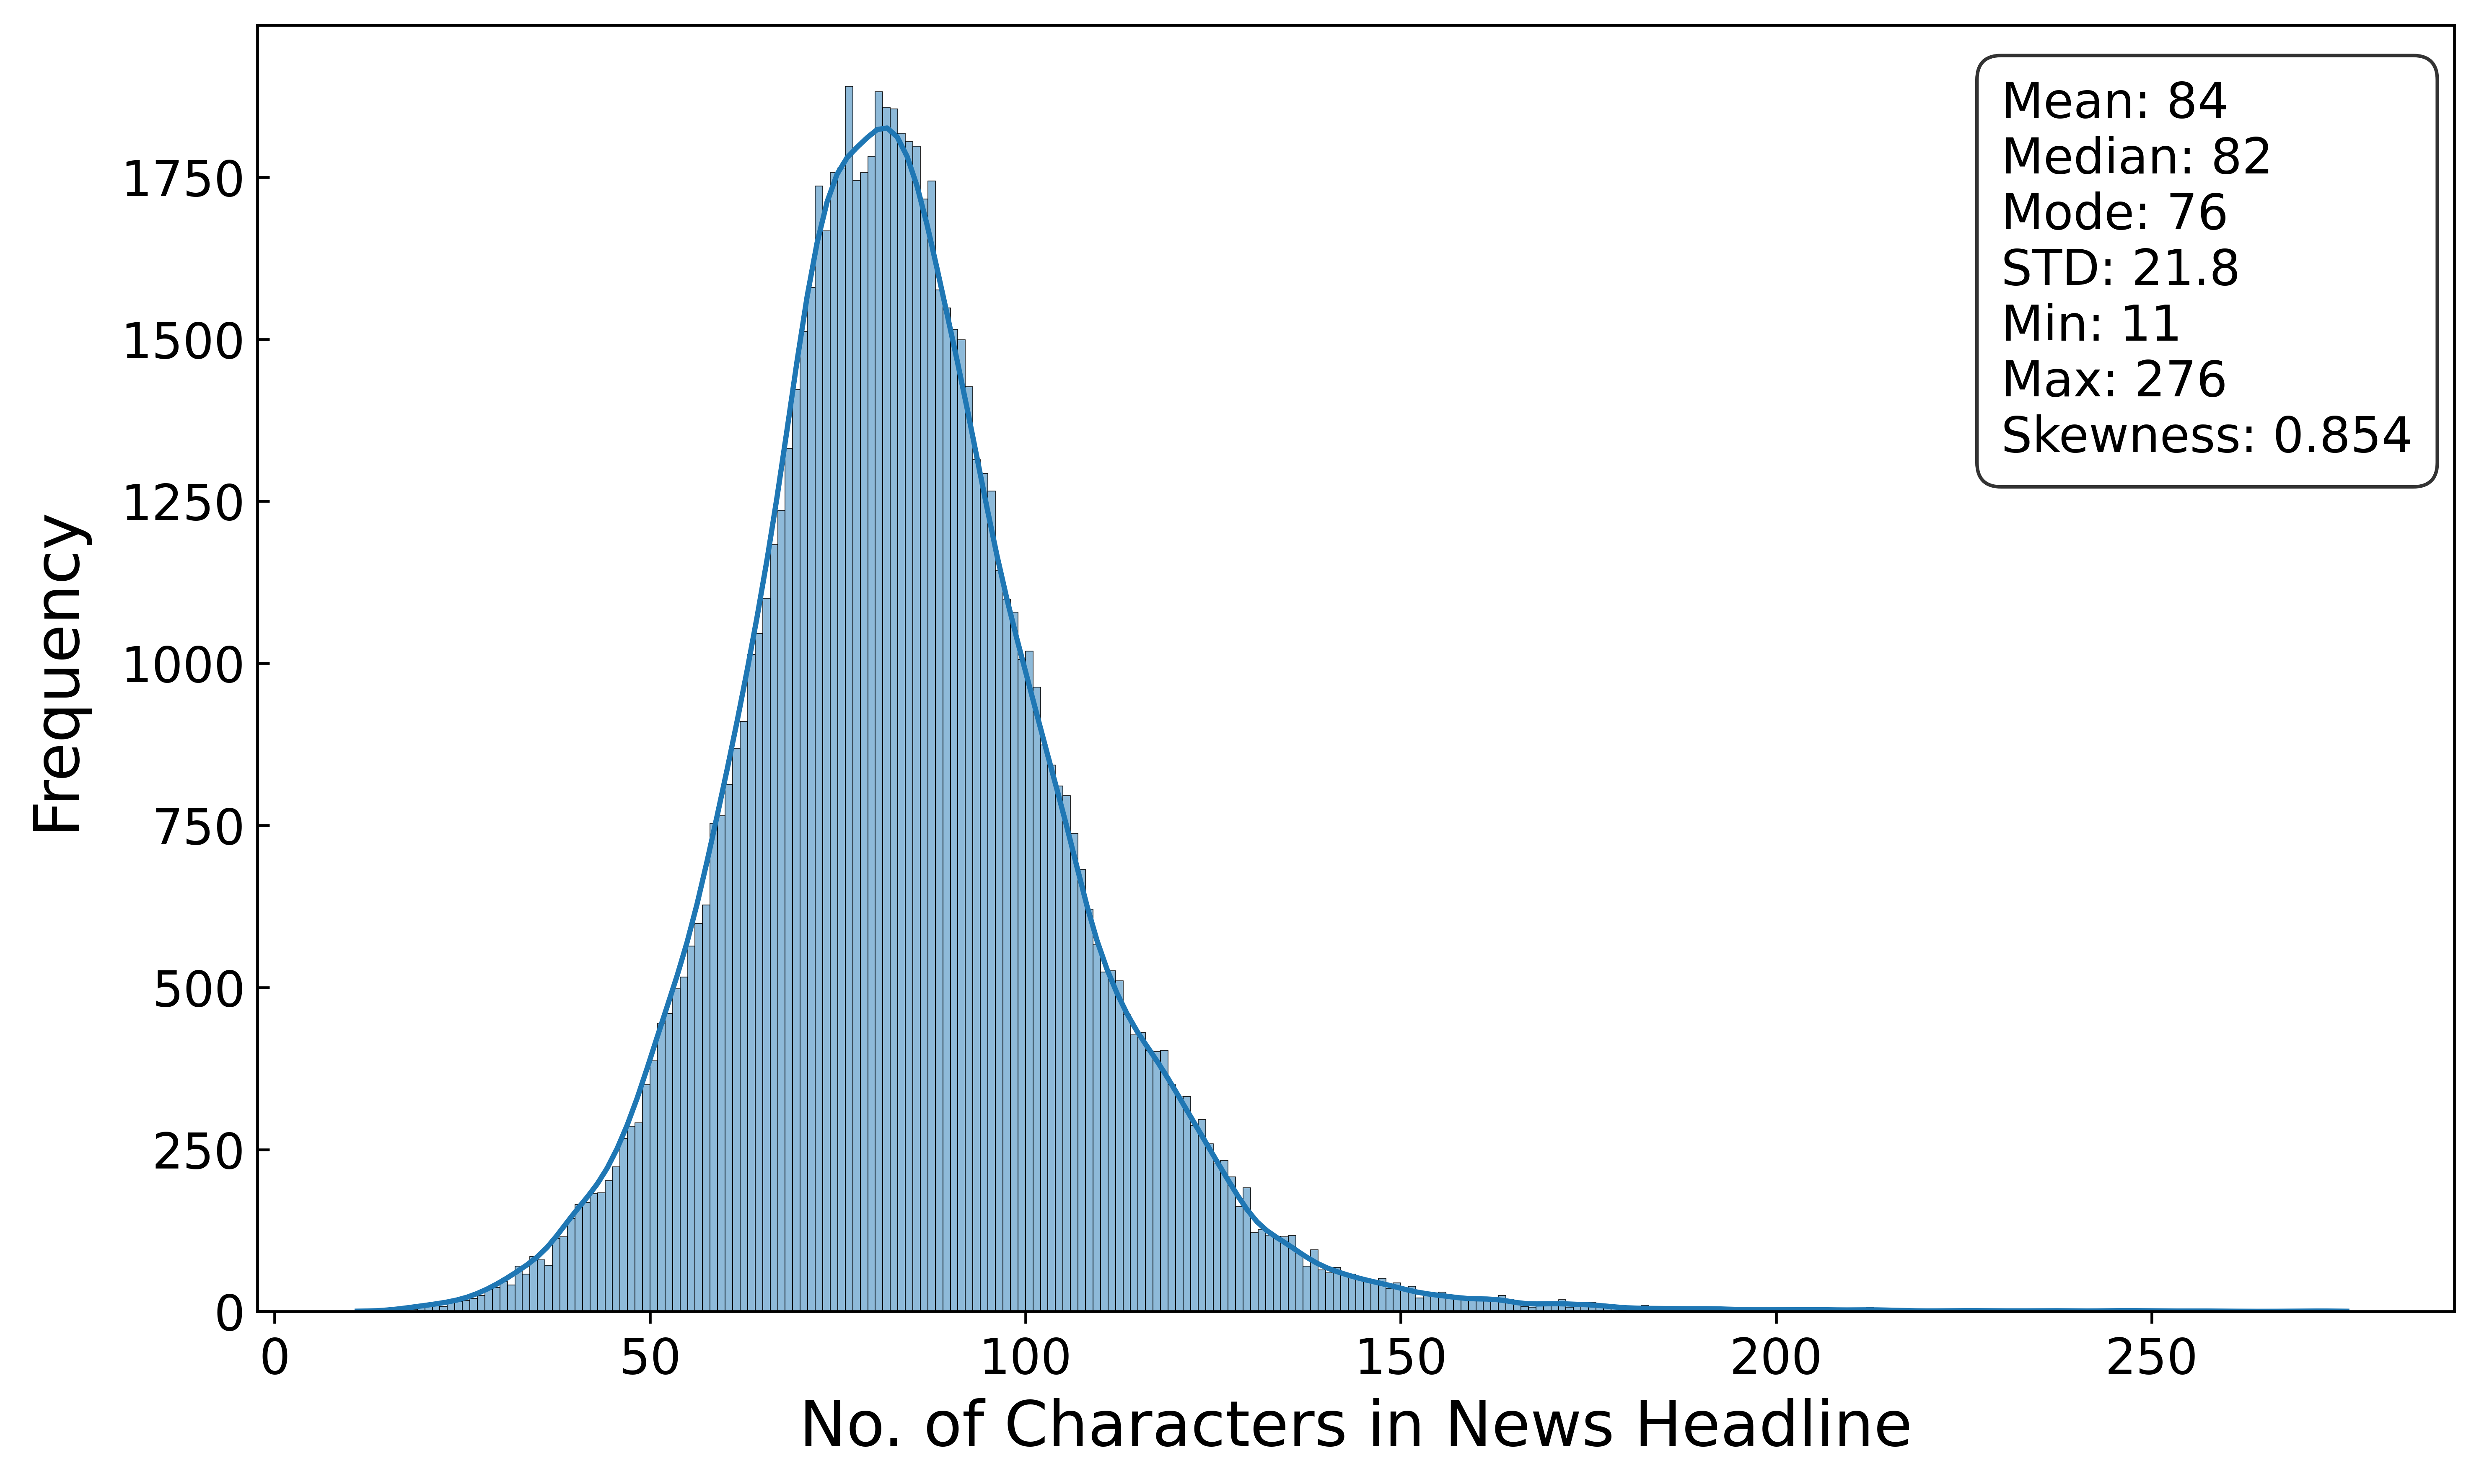
\includegraphics[width=0.8\linewidth]{figures/headline_length_distribution.png}
    \caption{Distribution of news headline length.}
    \label{fig:headline_length_distribution}
\end{figure}

The final analysis is that of the target itself - ETH prices - to understand its time series profile. The first aspect of the profile is to understand how previous prices are correlated with the present value. This is achieved by applying the autocorrelation function\footnote{Measures the correlation of a time series and its lagged values, including effects of all intermediary lags, e.g. correlation between $y_t$ and $y_{t-2}$ also includes effect of $y_{t-1}$ where \textit{t} is the current time step.} (ACF) and the partial autocorrelation function\footnote{Measures the correlation between two points, excluding effects of all intermediary time steps.} (PACF). However, the application of the above functions requires the time series to be stationary. To make a time series stationary, a feedback loop is needed between checking for stationarity and applying differencing\footnote{Subtracting the previous value from the current value in the time series for each time step - repeating this process on each differenced time series increases the differencing order by 1.} (\textit{d}), iterating the process until the series meets the stationarity criteria. Stationarity can be measured in many different ways; however, the most common ways include the use of the Augmented Dickey-Fuller (ADF) test and/or the Phillips-Perron (PP) test \cite{petricua2017stationarity}. The difference between the two is that the former does not account for heteroscedasticity in the time series, whilst the latter does. For both of the statistical tests, the null hypothesis assumes non-stationarity \cite{petricua2017stationarity}. Table \ref{tab:stationarity_check_matrix} contains the \textit{p} values of the tests as differencing was iteratively applied. After applying differencing only once, the \textit{p} values are less than 0.05, which rejects the null hypothesis and proves that the time series has become stationary. 

\begin{table}[ht]
\centering
\caption{\textit{p} values at various orders of differencing.}
\label{tab:stationarity_check_matrix}
\begin{tabular}{lcc}
\toprule
\multicolumn{1}{c}{} & \textbf{\textit{d} = 0} & \textbf{\textit{d} = 1} \\
\midrule
\textbf{ADF} & \textcolor{red}{\num{0.240}} & \textcolor{green!50!black}{\num{3.46E-22}} \\
\textbf{PP} & \textcolor{red}{\num{0.188}} & \textcolor{green!50!black}{0} \\
\bottomrule
\end{tabular}
\end{table}

Using this differenced time series, both ACF and PACF were applied to produce Figure \ref{fig:acf} and \ref{fig:pacf}, respectively. The blue shaded region shows the confidence interval band, and any spike exceeding that threshold is a statistically significant autocorrelation or partial autocorrelation lag. From the figures, ACF is continuously significant only up to the $1^{\text{st}}$ lag, and PACF is up to the $7^{\text{th}}$ lag. This suggests that the past ETH prices do not strongly predict future values beyond a very short lag, which is typical since most financial price levels behave close to a random walk \footnote{The current value $y_t$ is the sum of the previous value $y_{t-1}$ and some random error term $\varepsilon_t$.}.

\captionsetup[figure]{justification=centering}
\noindent
\begin{minipage}{0.49\textwidth}
    \begin{figure}[H]
        \centering
        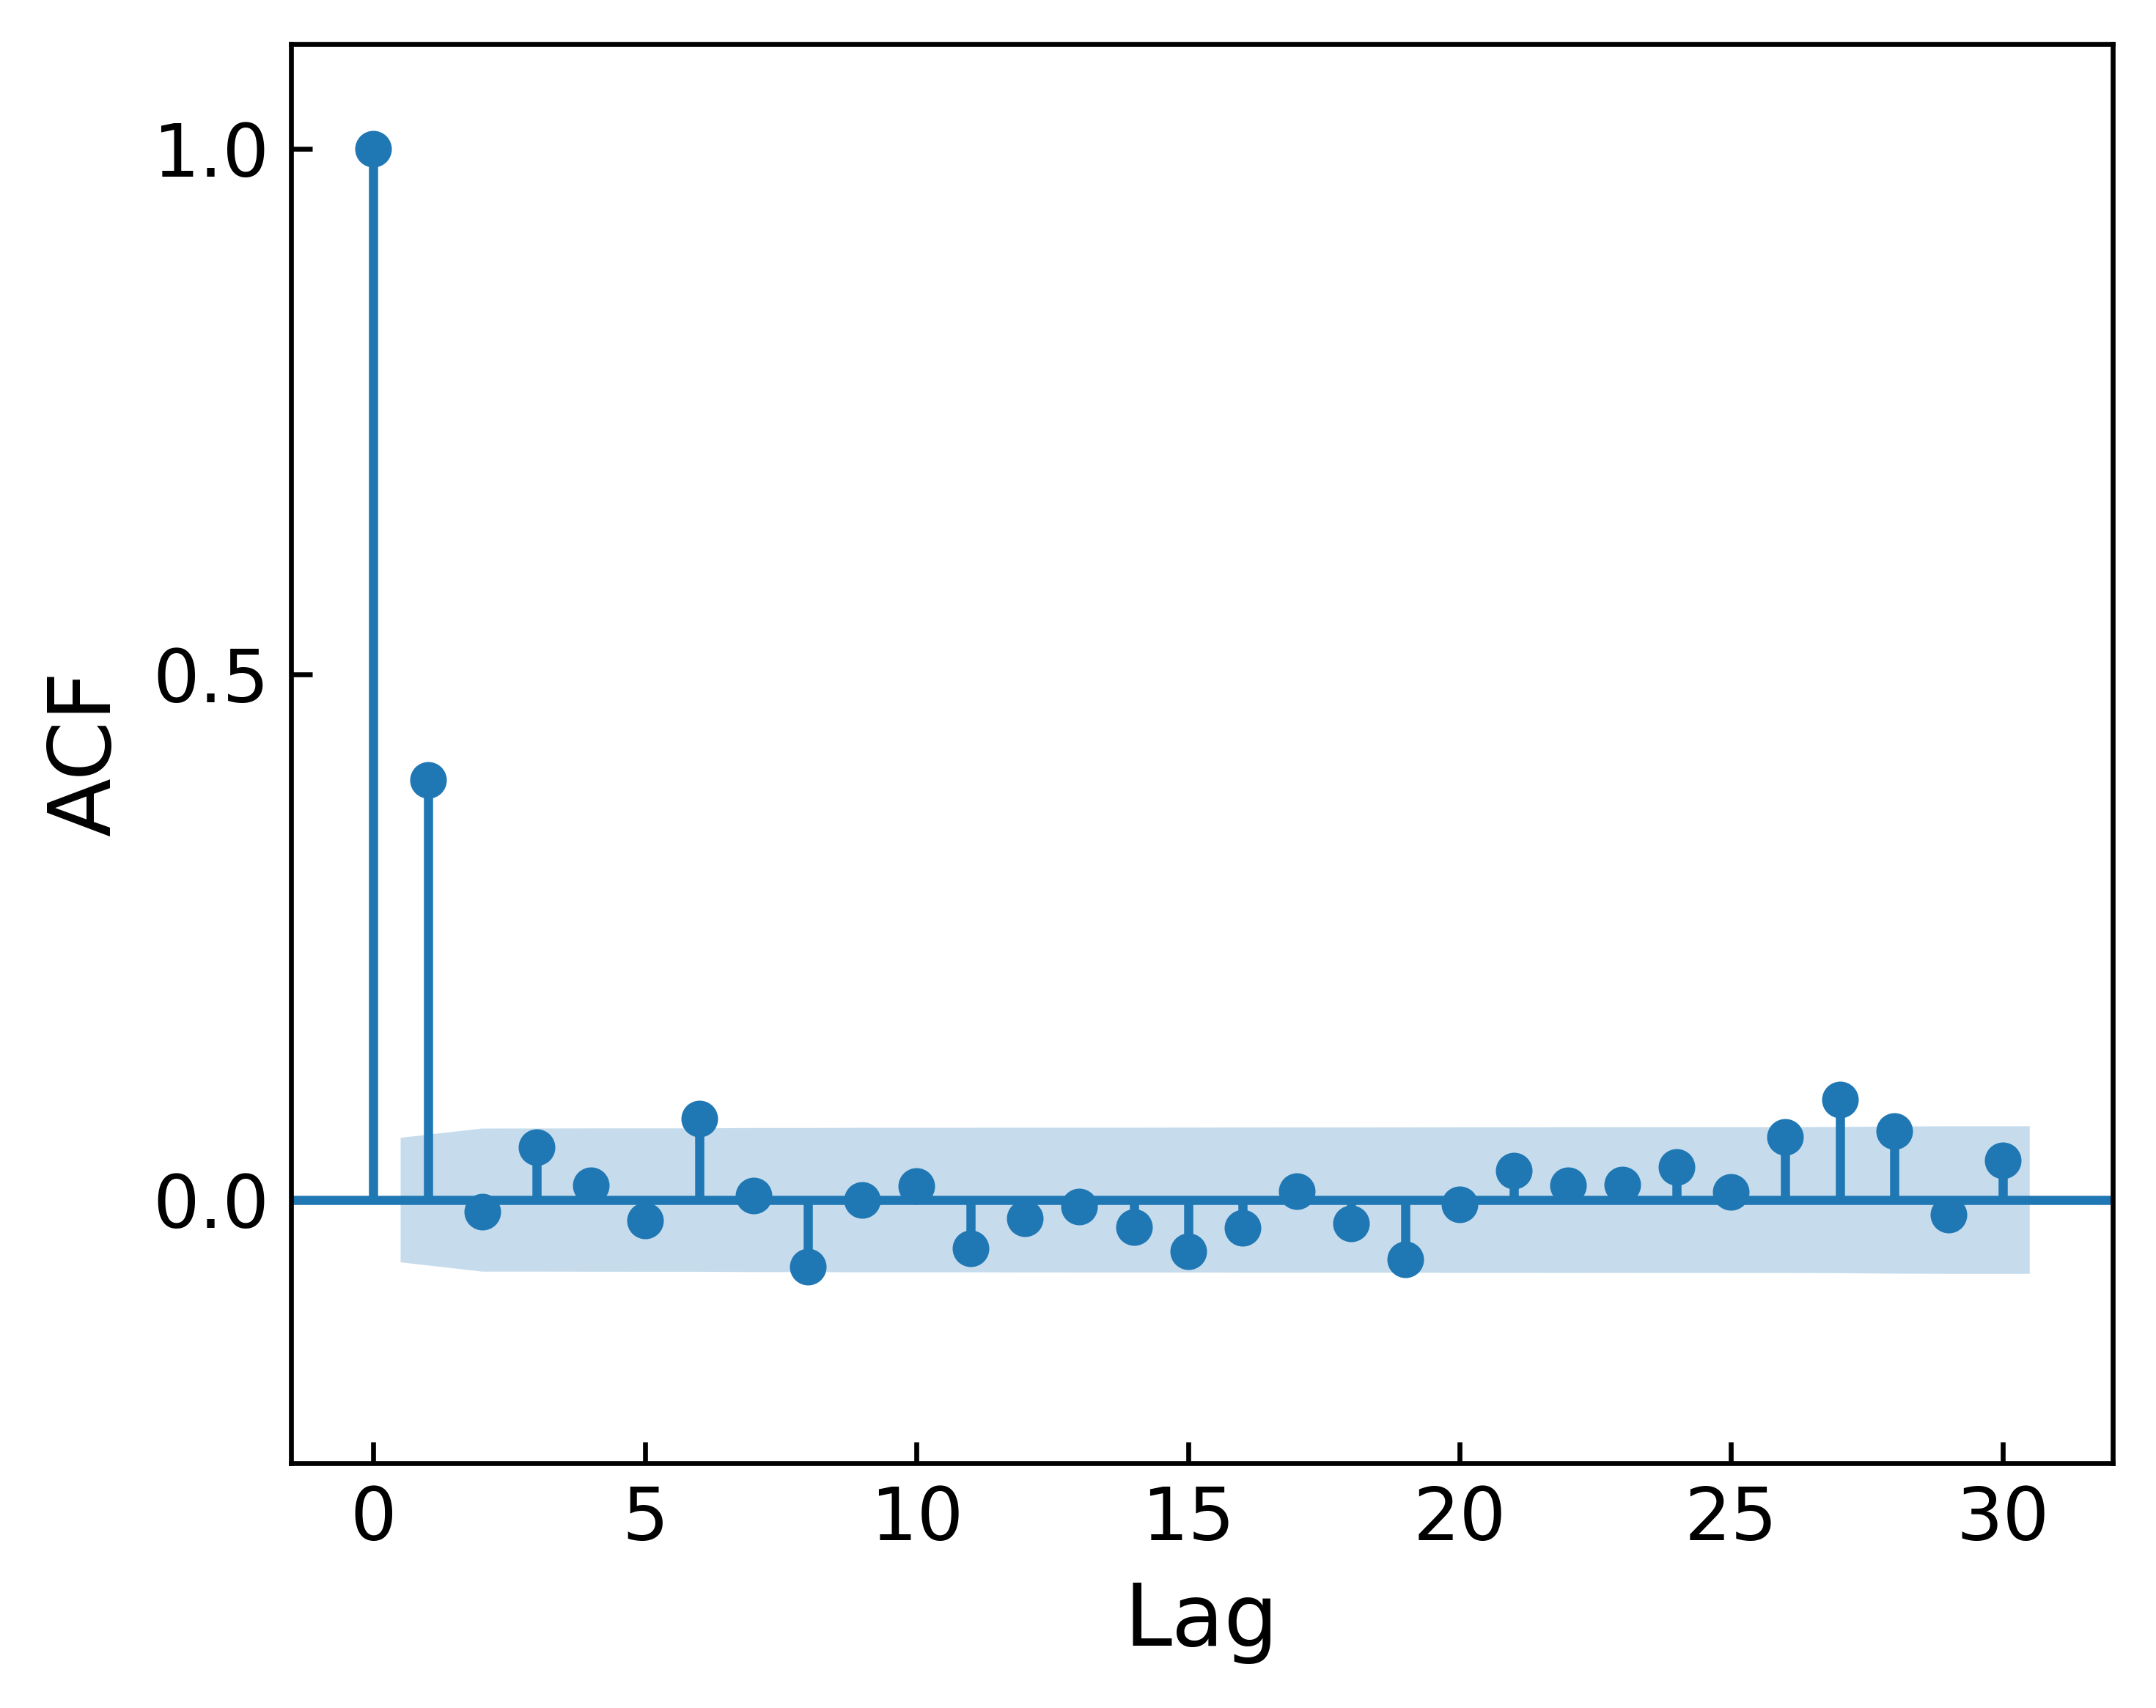
\includegraphics[width=\linewidth]{figures/acf.png}
        \captionof{figure}{ACF for 30 days of lag.}
        \vspace{0.7cm}
        \label{fig:acf}
    \end{figure}
\end{minipage}
\hfill
\begin{minipage}{0.49\textwidth}
    \begin{figure}[H]
        \centering
        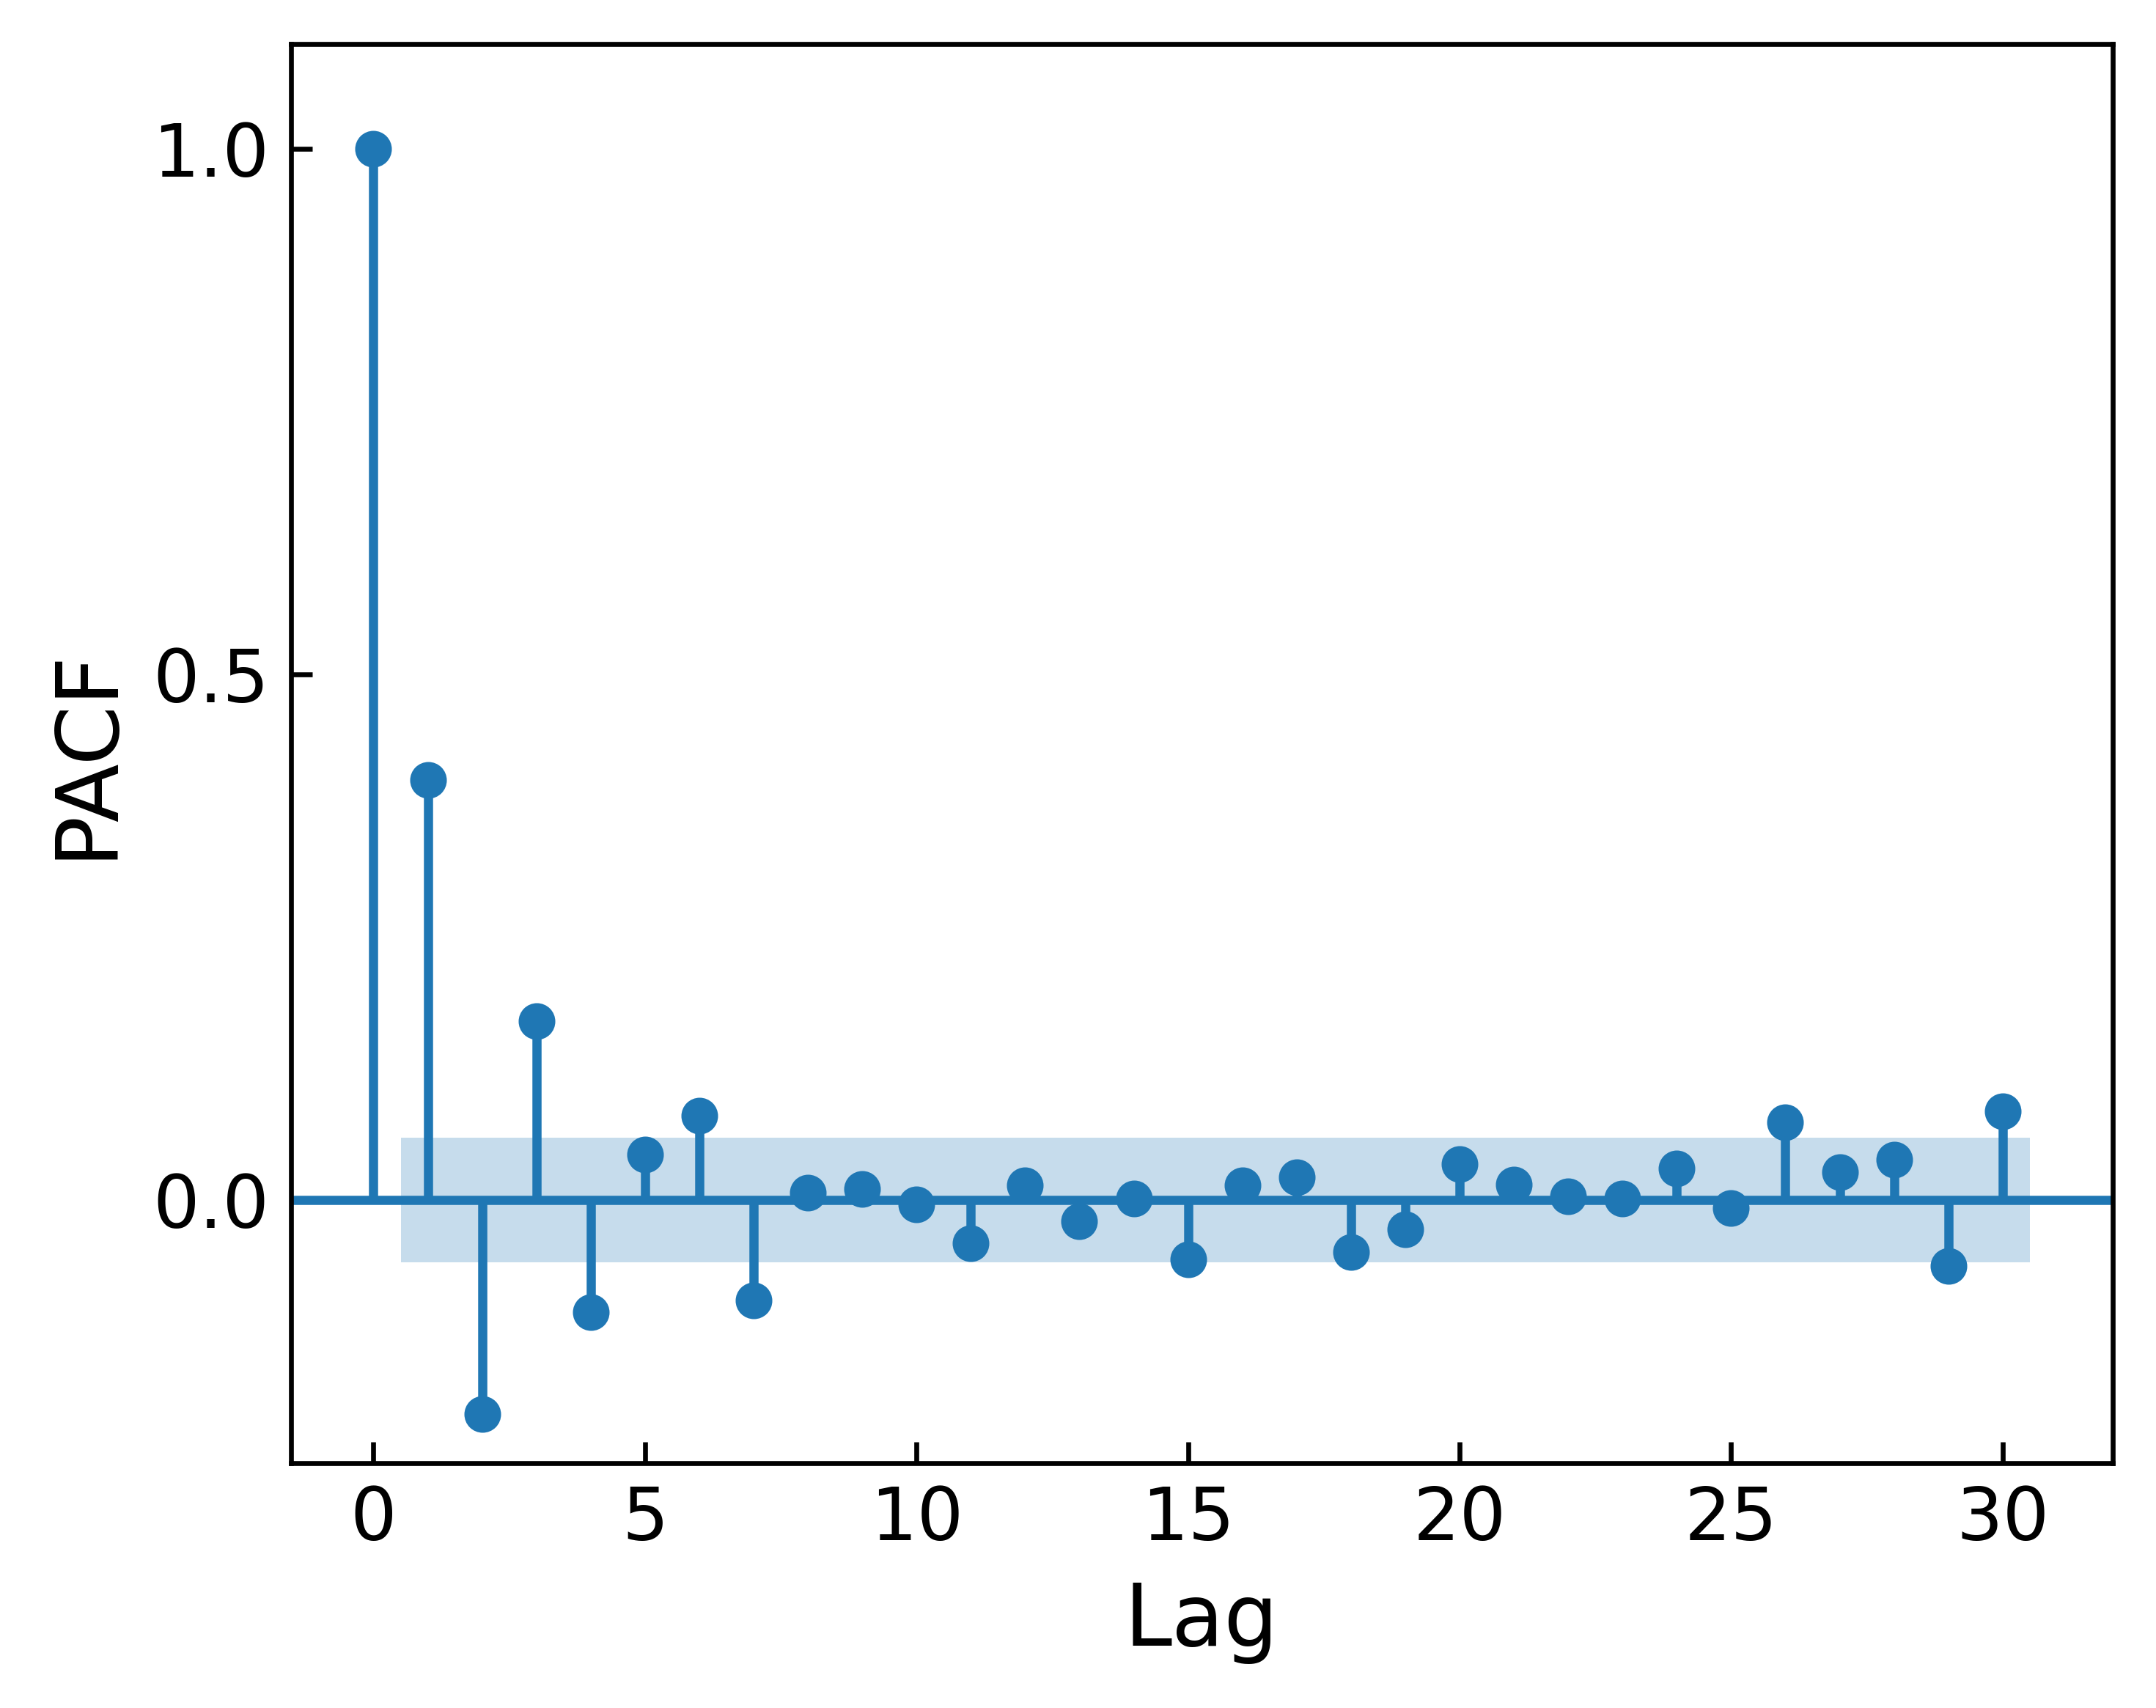
\includegraphics[width=\linewidth]{figures/pacf.png}
        \captionof{figure}{PACF for 30 days of lag.}
        \vspace{0.7cm}
        \label{fig:pacf}
    \end{figure}
\end{minipage}

 Another thing that can also be speculated from the ACF graph is seasonality. However, since there is no spike at a regular interval, it suggests there is likely weak seasonality, if at all. To further consolidate that, a time series can undergo a Seasonal-Trend decomposition using Loess smoothing (STL). In comparison to a classical Seasonal-Trend decomposition, STL has the advantage of being able to handle changing seasonality and is also more robust to outliers \cite{Hyndman2018}. Regardless of the method, the main assumption is that the time series consists of three components: trend ($T$), seasonality ($S$), and residual ($R$) \cite{Hyndman2018}. Trend and seasonality are self-explanatory, but residual accounts for noise and any variation unexplained by the former two components. For the decomposition, either all of the components are assumed to be summed (additive model) or multiplied (multiplicative model) with one another \cite{Hyndman2018}. In the case of ETH prices, a multiplicative model is more appropriate to account for any heteroscedasticity \cite{Hyndman2018} as shown by the fluctuating 7-day rolling standard deviation in Figure \ref{fig:stl}. Given that the STL method can only handle additive models, the prices were first log transformed to stabilise the variance, but also so that the transformed time series can be treated as an additive model \cite{Hyndman2018}. Moreover, as part of the STL, the input argument was 7 days, assuming an intraweek seasonality pattern due to the findings from \cite{jasiak2024intraday}. Figure \ref{fig:stl} shows the three components along with the original untransformed ETH prices for the selected date range. The strength of the (intraweek) seasonality ($F_S$) can be calculated using Equation \ref{eq:component_strength} \cite{Hyndman2018}, where the variance of the residual and seasonal components is used. Similarly, the strength of the trend ($F_T$) can be calculated using the same equation by replacing the $S$ with $T$ \cite{Hyndman2018}. The nature of this equation gives a value between 0 and 1 because the fractional term is expected to be small \cite{Hyndman2018}. In the case where the variance of the numerator is much larger than that of the denominator in the fractional term, the max function forces a lower bound of 0. Contrary to \cite{jasiak2024intraday}, the decomposition has an $F_S$ of 0.26, suggesting weak intraweek seasonality pattern. This evidence means that creating a categorical feature representing the days of the week would not be as useful as initially assumed. Analysing the residual component, it is clear that the multiplicative model is appropriate, given the values are very small, albeit erratic, around 0. The fluctuation of residuals between 2021 to late 2022 is more aggressive than the remaining timeline, implying the presence of higher volatility, anomalies and/or structural breaks between 2021 and 2022.

\begin{figure}[H]
    \centering
    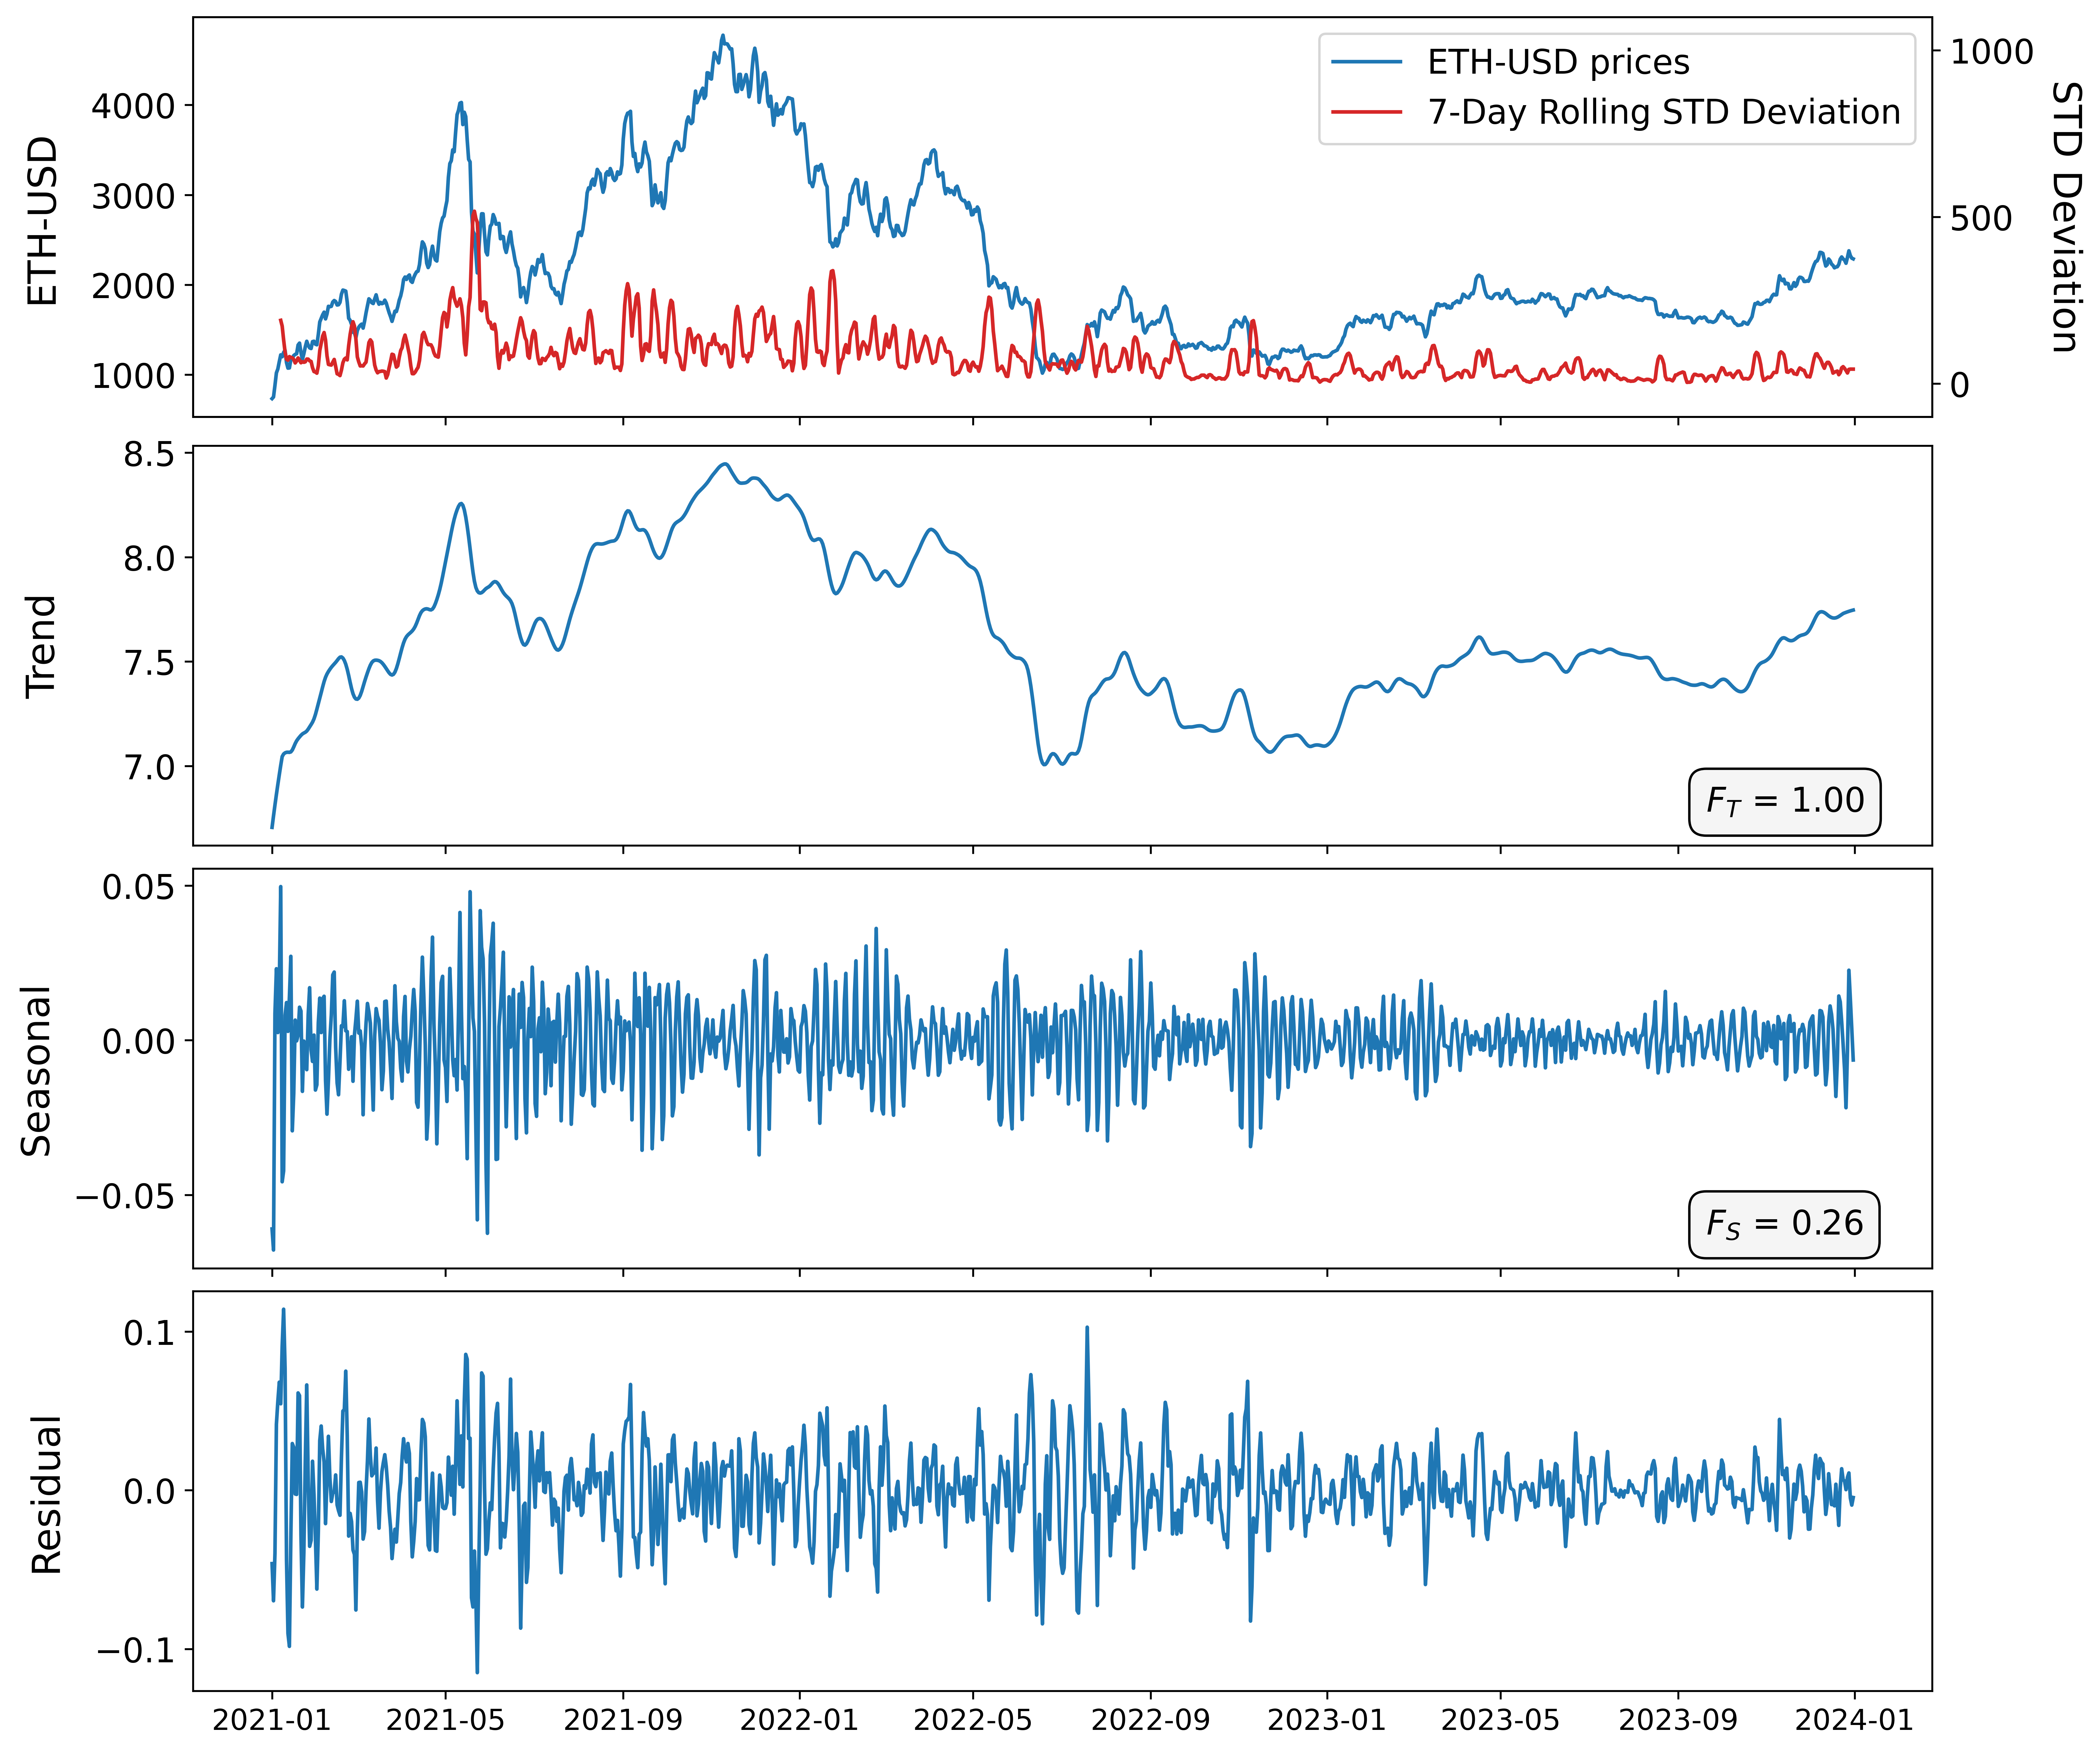
\includegraphics[width=1\linewidth]{figures/stl.png}
    \caption{Seasonal-trend decomposition using Loess smoothing.}
    \label{fig:stl}
\end{figure}

\begin{equation}
\label{eq:component_strength}
F_S = max\left(0, 1 - \frac{Var(R)}{Var(S + R)}\right) 
\end{equation}

% -----------------------------------------------------------------------------

\chapter{Methodology}
\label{chap:methodology}

This chapter aims to highlight the key steps of the methodology. At a high level, Figure \ref{fig:methodology_flowchart} summarises the methodology as a 7-step process that will be explained further in the sections of this chapter.

\begin{figure}[H]
    \centering
    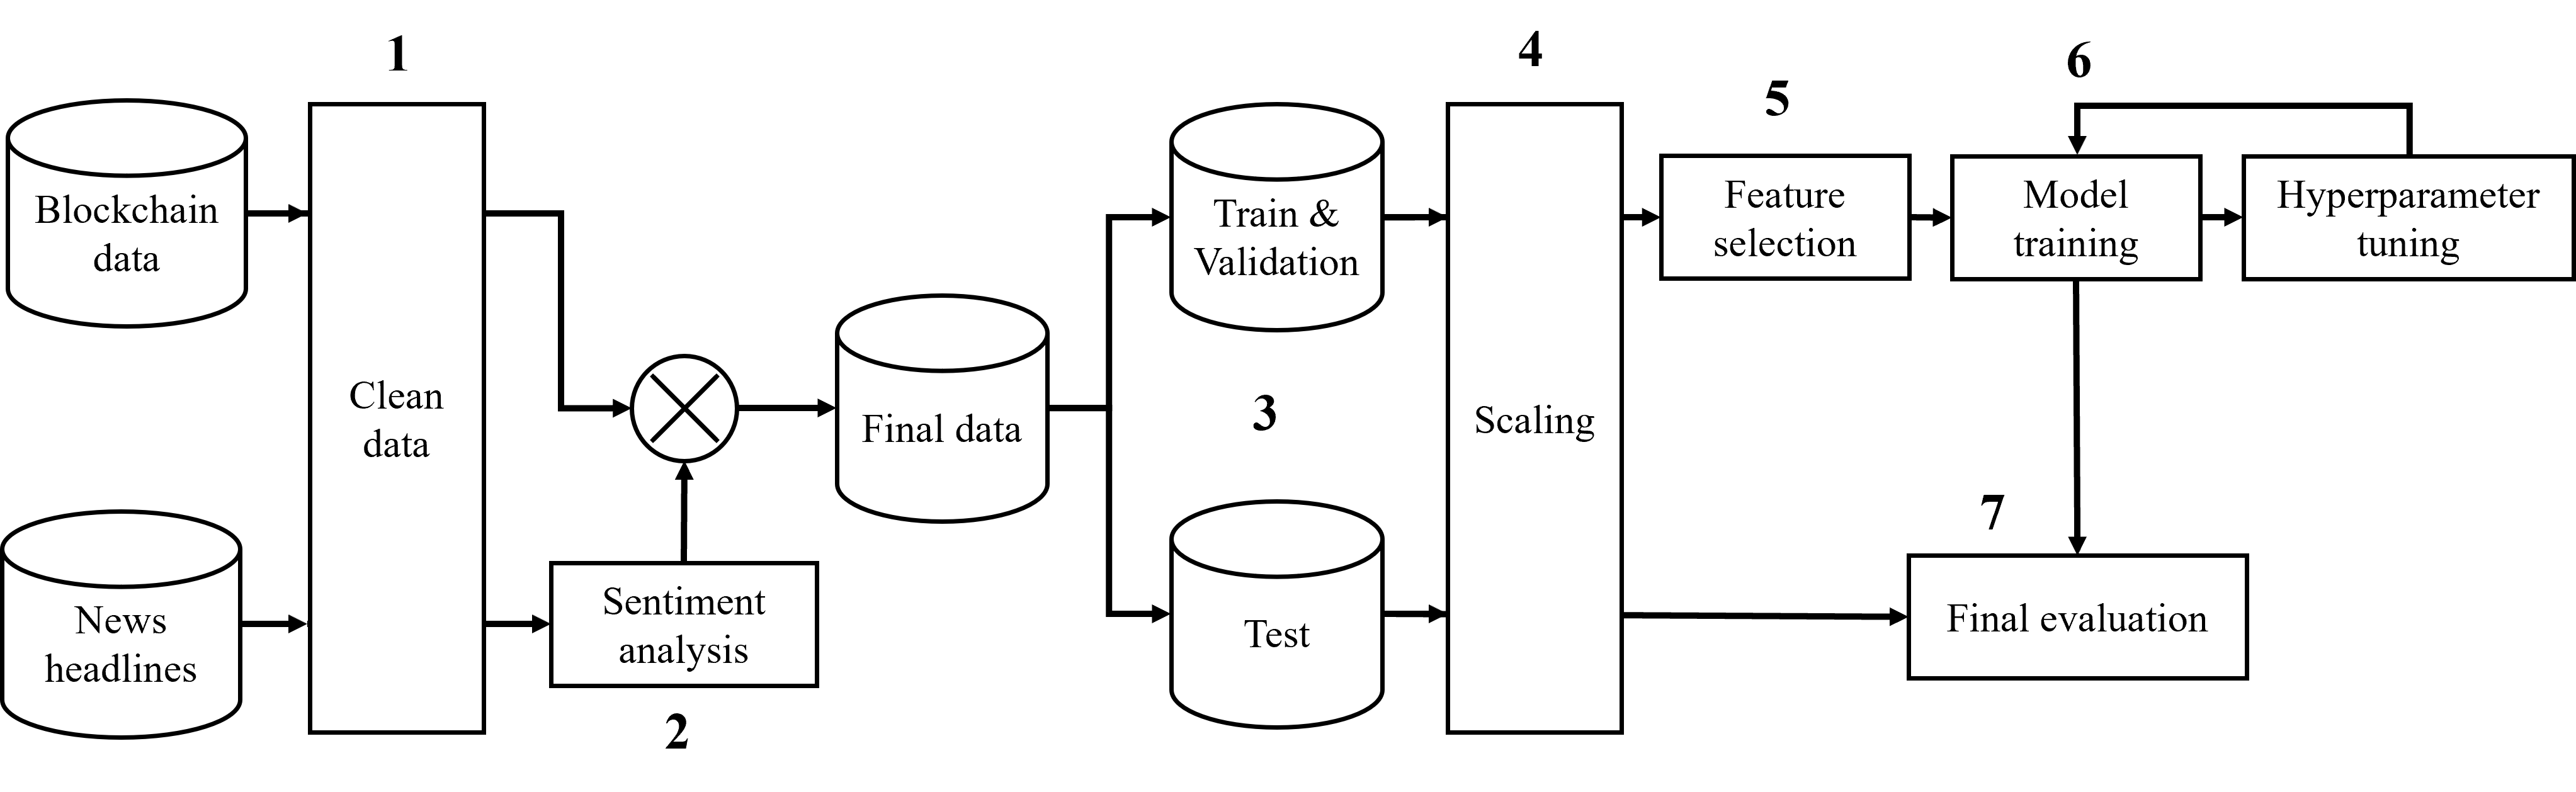
\includegraphics[width=1\linewidth]{figures/methodology_flowchart.png}
    \caption{Methodology flowchart.}
    \label{fig:methodology_flowchart}
\end{figure}

\section{Data Cleaning}
The first aspect of data cleaning involved imputing missing blockchain data. Given that there was a very small proportion of missing data, a simple time-weighted linear interpolation was conducted as provided by the \texttt{interpolate()} method in the \texttt{Pandas} Python library. 

The second aspect of data cleaning involved preparing the news headlines for sentiment analysis. Some news headlines were found to consist of mojibake as a result of incorrect decoding of text during the download; therefore, during the reading operation, the data was UTF-8 encoded. Another cleaning process involved removing any extremely long headlines that are not truly headlines. Since the mean of the distribution in Figure \ref{fig:headline_length_distribution} was 84, assuming a symmetrical distribution, any headlines longer than 168 characters were manually looked at and filtered. Consequently, all the headlines were valid, and the distribution was naturally just positively skewed. 

\section{Sentiment Analysis}
\label{sec:sentiment_analysis}
One of the most widely used lexicon-based methods is \textbf{V}alence \textbf{A}ware \textbf{D}ictionary for s\textbf{E}ntiment \textbf{R}easoning (VADER) \cite{kumar2025evolving,hutto2014vader}. It is a rule-based dictionary with words classified as positive or negative, and can also handle punctuation and emojis to increase the sentiment's intensity \cite{RN104}. Some of its advantages are that it is fast, easy to interpret, and suitable for analysing short texts such as news headlines, making it ideal for a baseline. The way it classifies the overall sentiment of a text is by producing a compound score that takes a normalised (1 to -1) sum of all lexicons \cite{RN104}. Where a score greater than 0.05 is considered positive, a score less than -0.05 is considered negative, and anything in between is neutral \cite{RN104}. 

Regarding pre-trained, fine-tuned transformers, there are two relevant to this project: FinBERT \cite{araci2019finbert} and CryptoBERT \cite{kulakowski2023sentiment}. Both models are fine-tuned versions of the Bidirectional Encoder Representations from Transformers (BERT) - a pre-trained language model developed by Google \cite{kumar2025evolving}. FinBERT is fine-tuned using Financial PhraseBank (consists of a random set of 4,845 sentences from financial news) and TRC2-financial (consists of 46,143 documents from 1.8m news articles published by Reuters) \cite{araci2019finbert}. This makes FinBERT a strong candidate for experimentation. The output labels of FinBERT's sentiment analysis are ``positive", ``negative", and ``neutral", accompanied by a confidence score indicating the likelihood of the label being correct. CryptoBERT is fine-tuned on 3.207m social media posts from X (Twitter), Reddit, Telegram and StockTwits \cite{kulakowski2023sentiment}. Though the data for CryptoBERT is only social media, it was still considered a suitable candidate due to its specialisation in capturing the speculative language of cryptocurrencies. The output labels of CryptoBERT's sentiment analysis are ``bullish", ``bearish" and ``neutral", where the former two are synonymous with ``positive" and ``negative", respectively. Similar to FinBERT, it also provides a confidence score. 

Once the three types of sentiment analysis were conducted, the scores/labels needed to be filtered (to remove noise), and the scores were aggregated since there were multiple headlines collected for each day. The presence of neutral headlines was one of the factors contributing to the noise. Neutral headlines do not steer the price direction; as such, they were completely removed before aggregation. Another speculative factor contributing to the noise was the presence of news from less-known publishers, hence a smaller impact. To test this, the distribution of aggregated scores, thereby labels, was compared between the inclusion of all publishers and only the top 20. For VADER, the aggregation was done by taking the mean of the scores of all headlines at hand. For FinBERT and CryptoBERT, the labels were converted to their numerical equivalent, where positive was 1, negative was -1 and neutral was 0. Unlike VADER, BERT models do not have sentiment intensity, which is important in reducing the chances of the aggregated score being neutral. Therefore, the sentiment labels were multiplied by their confidence scores to artificially speculate the intensity. Finally, taking the mean of these intensity scores to get the final score of the day. For all sentiment analysers, any aggregated score greater than 0 was considered positive, and anything less than 0 was considered negative.

Analysing the distribution of classes in Figure \ref{fig:sentiment}, it can be seen that CryptoBERT and VADER classify the majority of days with a net positive sentiment. An initial comparison of this distribution to the price behaviour in Figure \ref{fig:stl} it is clear that prices are not just increasing, which could suggest that either the two sentiment methods are not accurate or the news headlines are not effective in capturing the price movement. Moreover, there is no significant difference in the distribution when comparing all publishers to only the top 20, as such sentiment from all publishers was used. 

\begin{figure}[H]
    \centering
    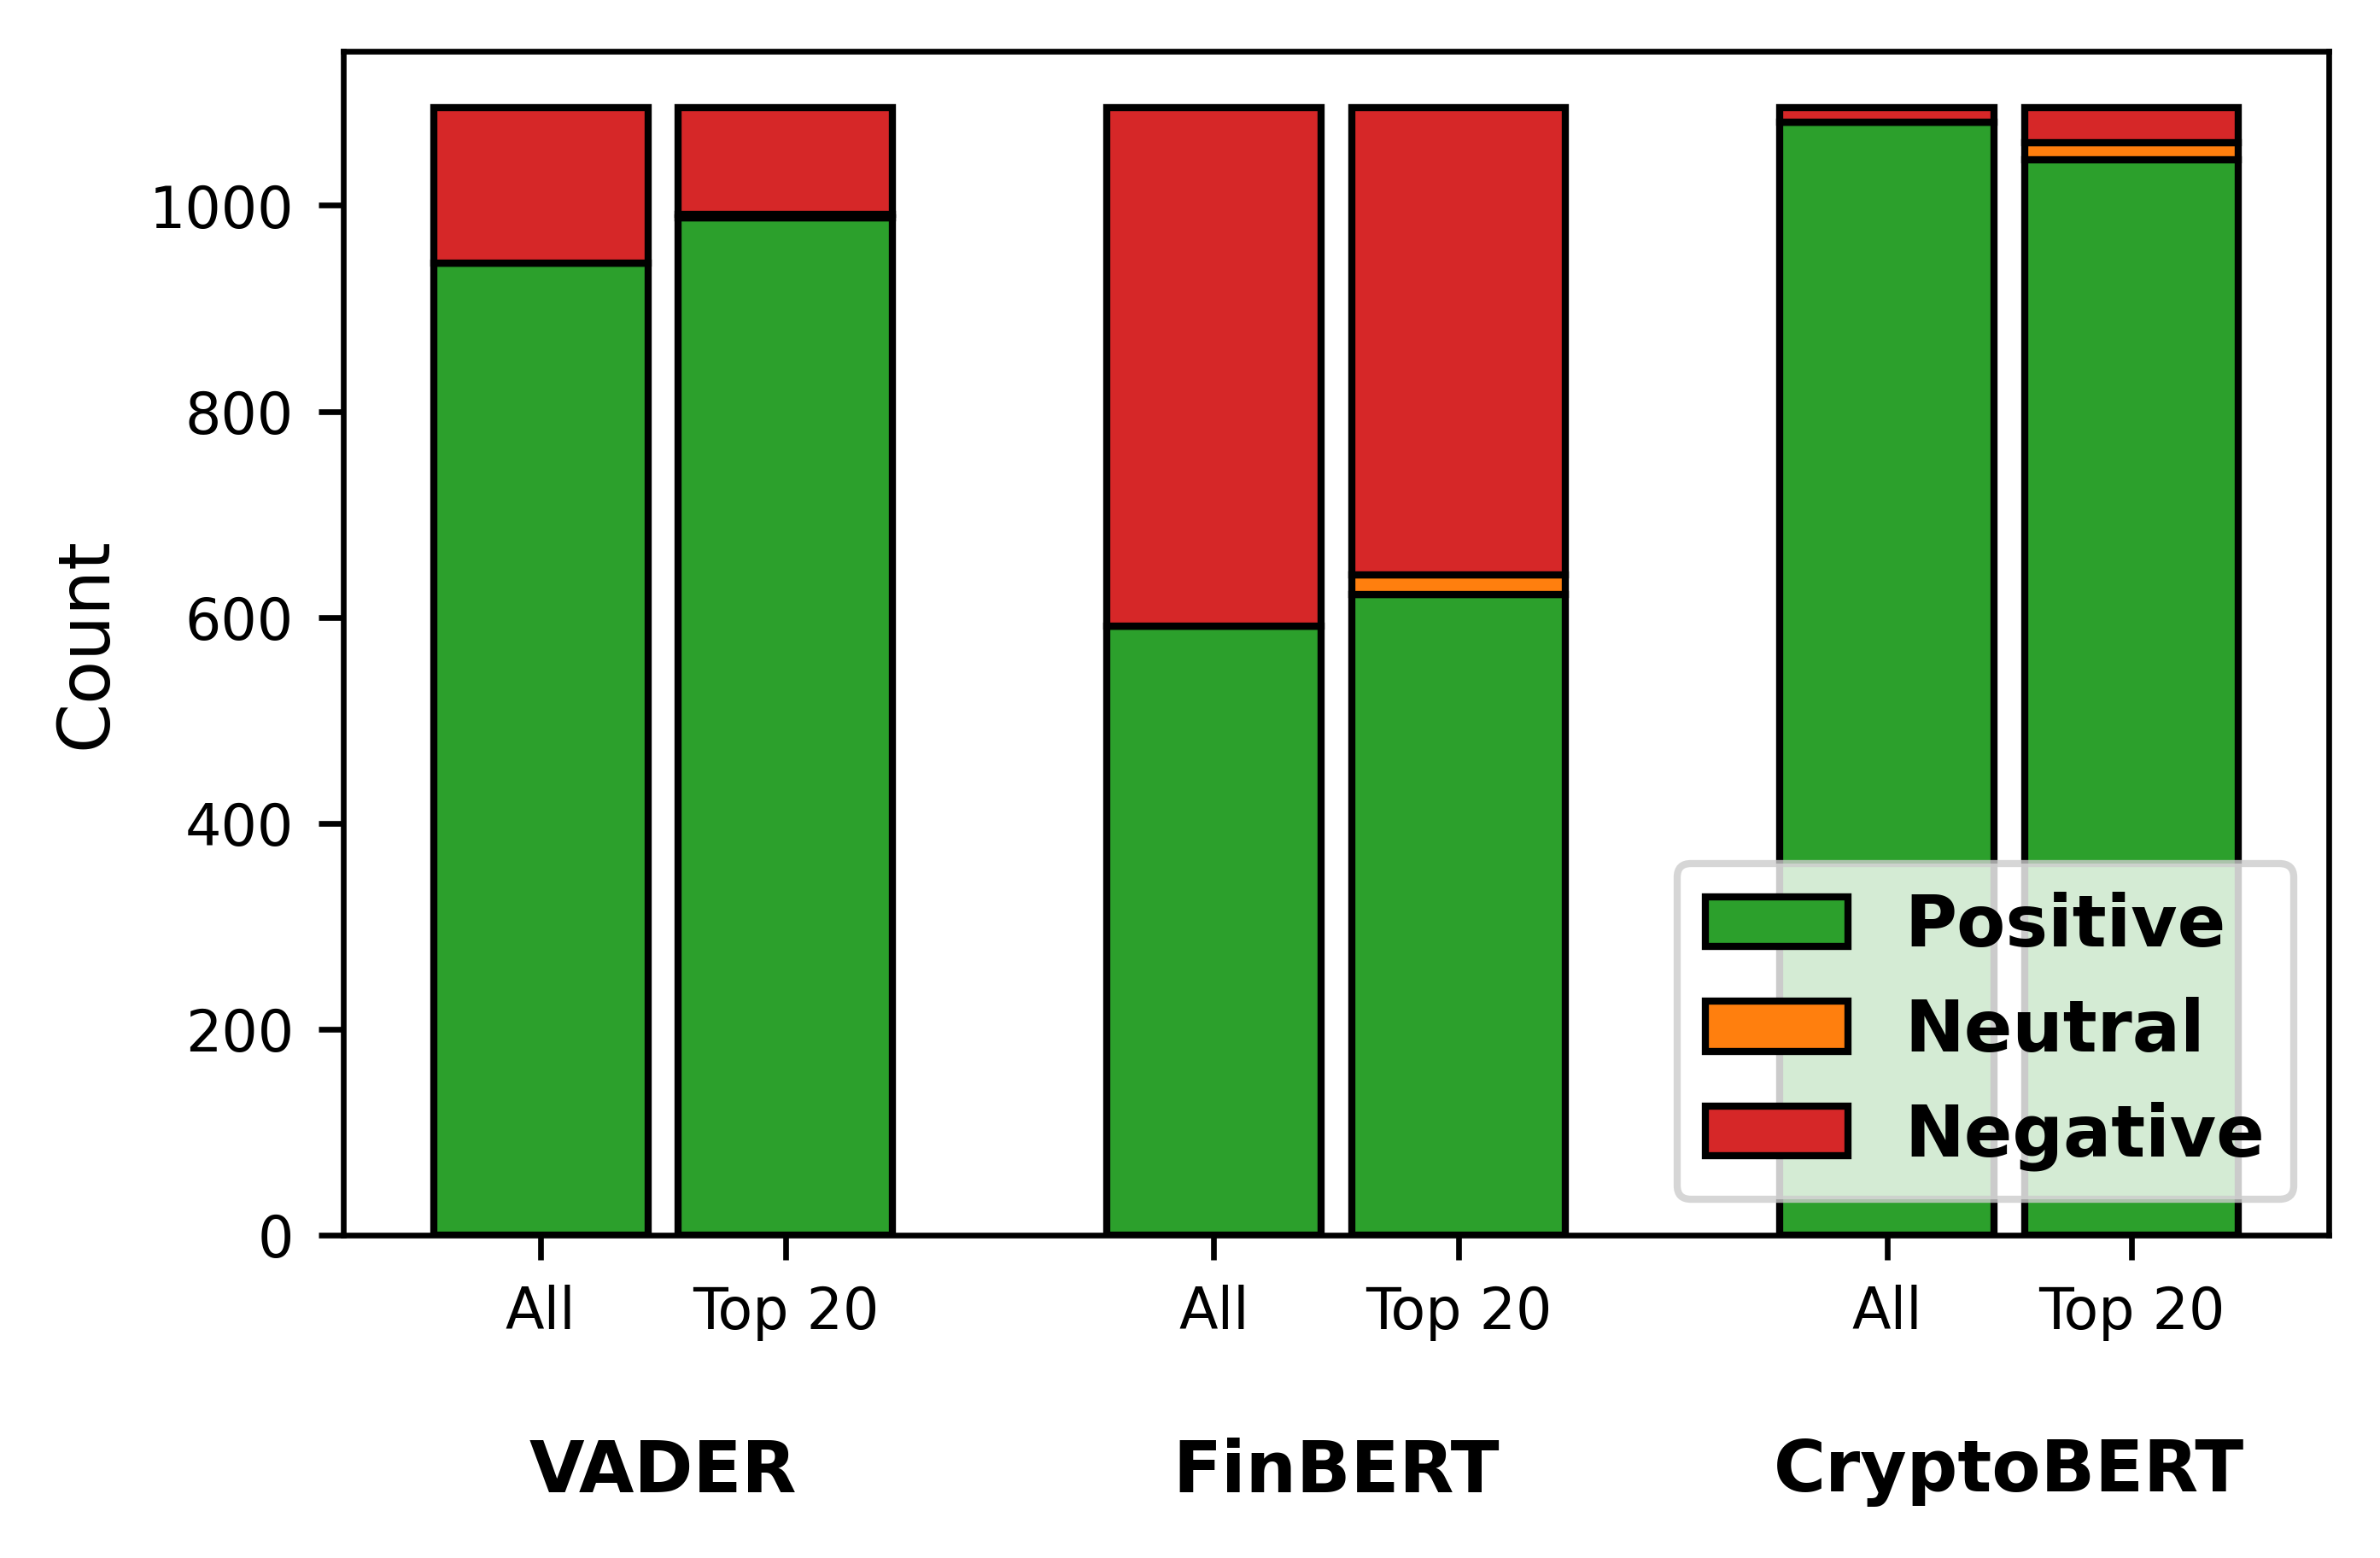
\includegraphics[width=0.7\linewidth]{figures/sentiment.png}
    \caption{Distribution of aggregated sentiment classification for different methods.}
    \label{fig:sentiment}
\end{figure}

% \noindent
% \begin{minipage}{0.49\textwidth}
%     \begin{figure}[H]
%         \centering
%         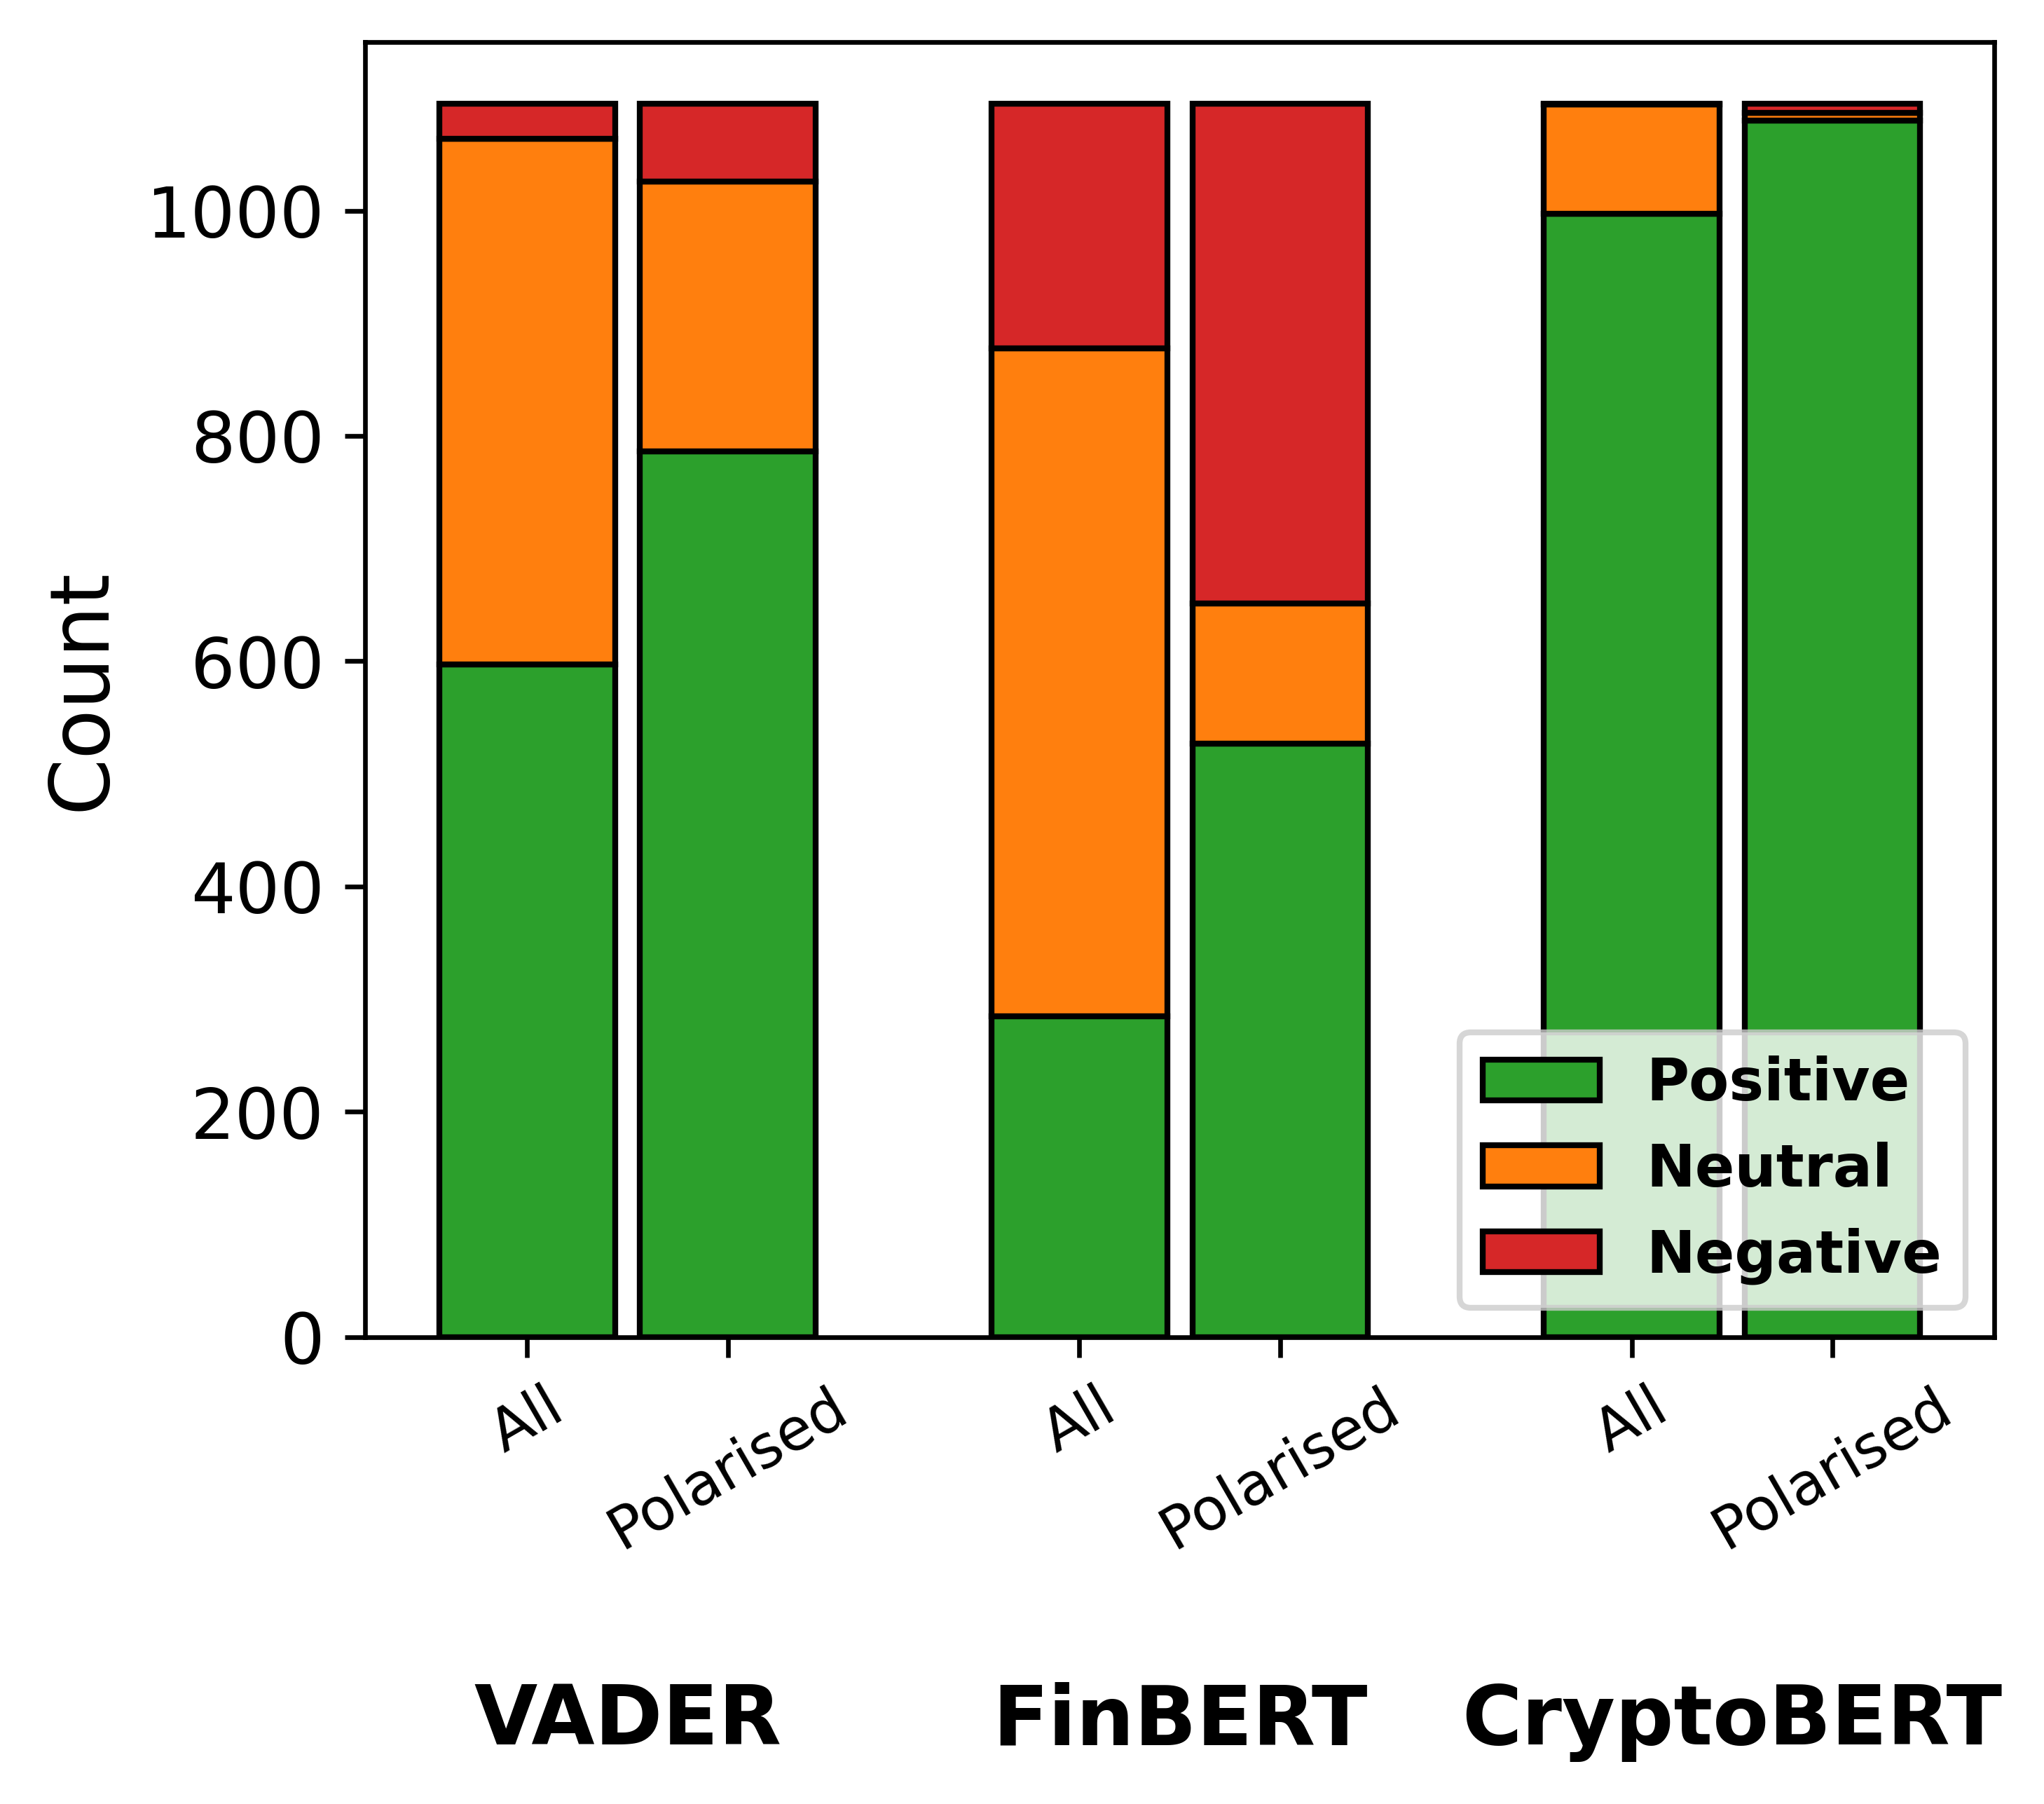
\includegraphics[width=\linewidth]{figures/all_pub.png}
%         \captionof{figure}{Comparison of all and polarised headlines only for all publishers.}
%         \vspace{0.3cm}
%         \label{fig:all_pub}
%     \end{figure}
% \end{minipage}
% \hfill
% \begin{minipage}{0.5\textwidth}
%     \begin{figure}[H]
%         \centering
%         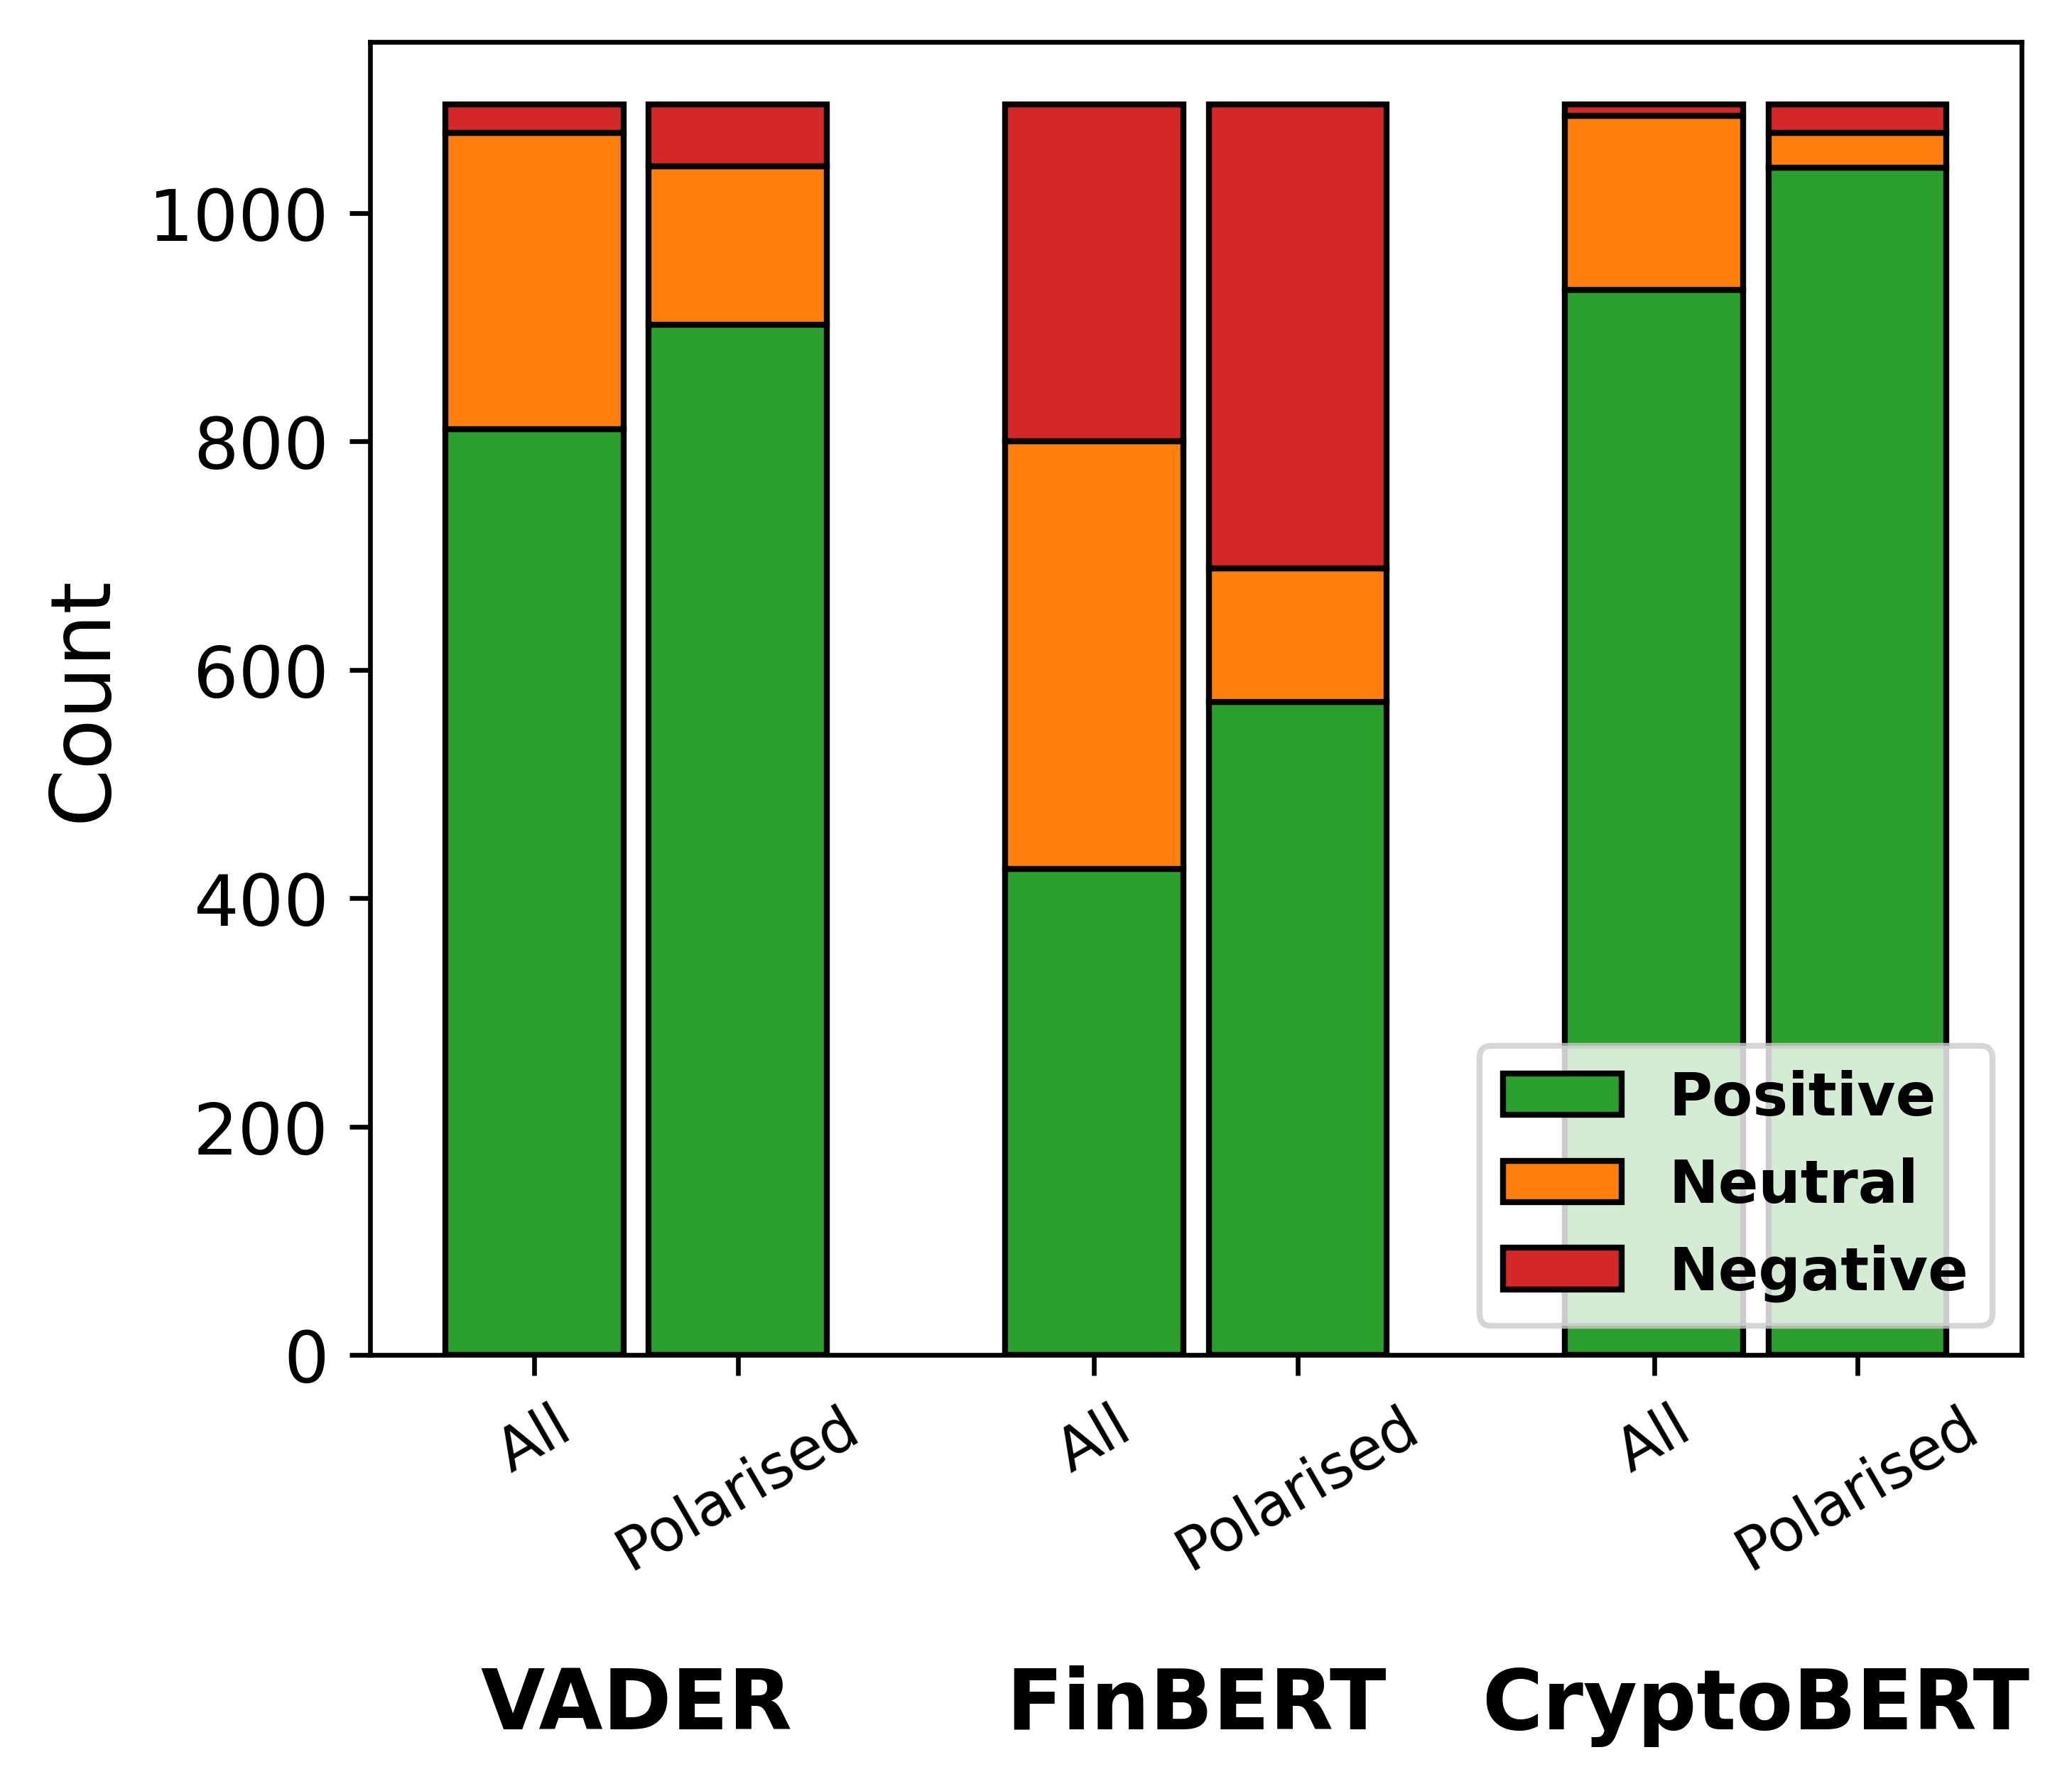
\includegraphics[width=\linewidth]{figures/top_20_pub.png}
%         \captionof{figure}{Comparison of all and polarised headlines only for the top 20 publishers.}
%         \vspace{0.3cm}
%         \label{fig:top_20_pub}
%     \end{figure}
% \end{minipage} 


\section{Data Partitioning}
\label{sec:data_partitioning}
To split the data, a slightly larger ratio of train to test was taken - 85:15. The reason for this was to increase the training size, given that DNNs benefit from more data. The training data was further split using the same ratio to create a validation set. Figure \ref{fig:test_train_validation} shows the three splits, with a 7-day gap\footnote{A gap is not needed for statistical models like ARIMA because they train purely on past values for forecasting.} between them to prevent data leakage. The gap size is in line with the forecasting horizon of 7 days. The reason for forecasting one week is to improve the real-world applicability of the model for traders, which is one of the gaps most cryptocurrency price prediction studies fail to address \cite{john2024cryptocurrency}. Having just a next-day forecast may not be as useful in setting up trading strategies, especially if the forecast shows a negligible return.

\begin{figure}[H]
    \centering
    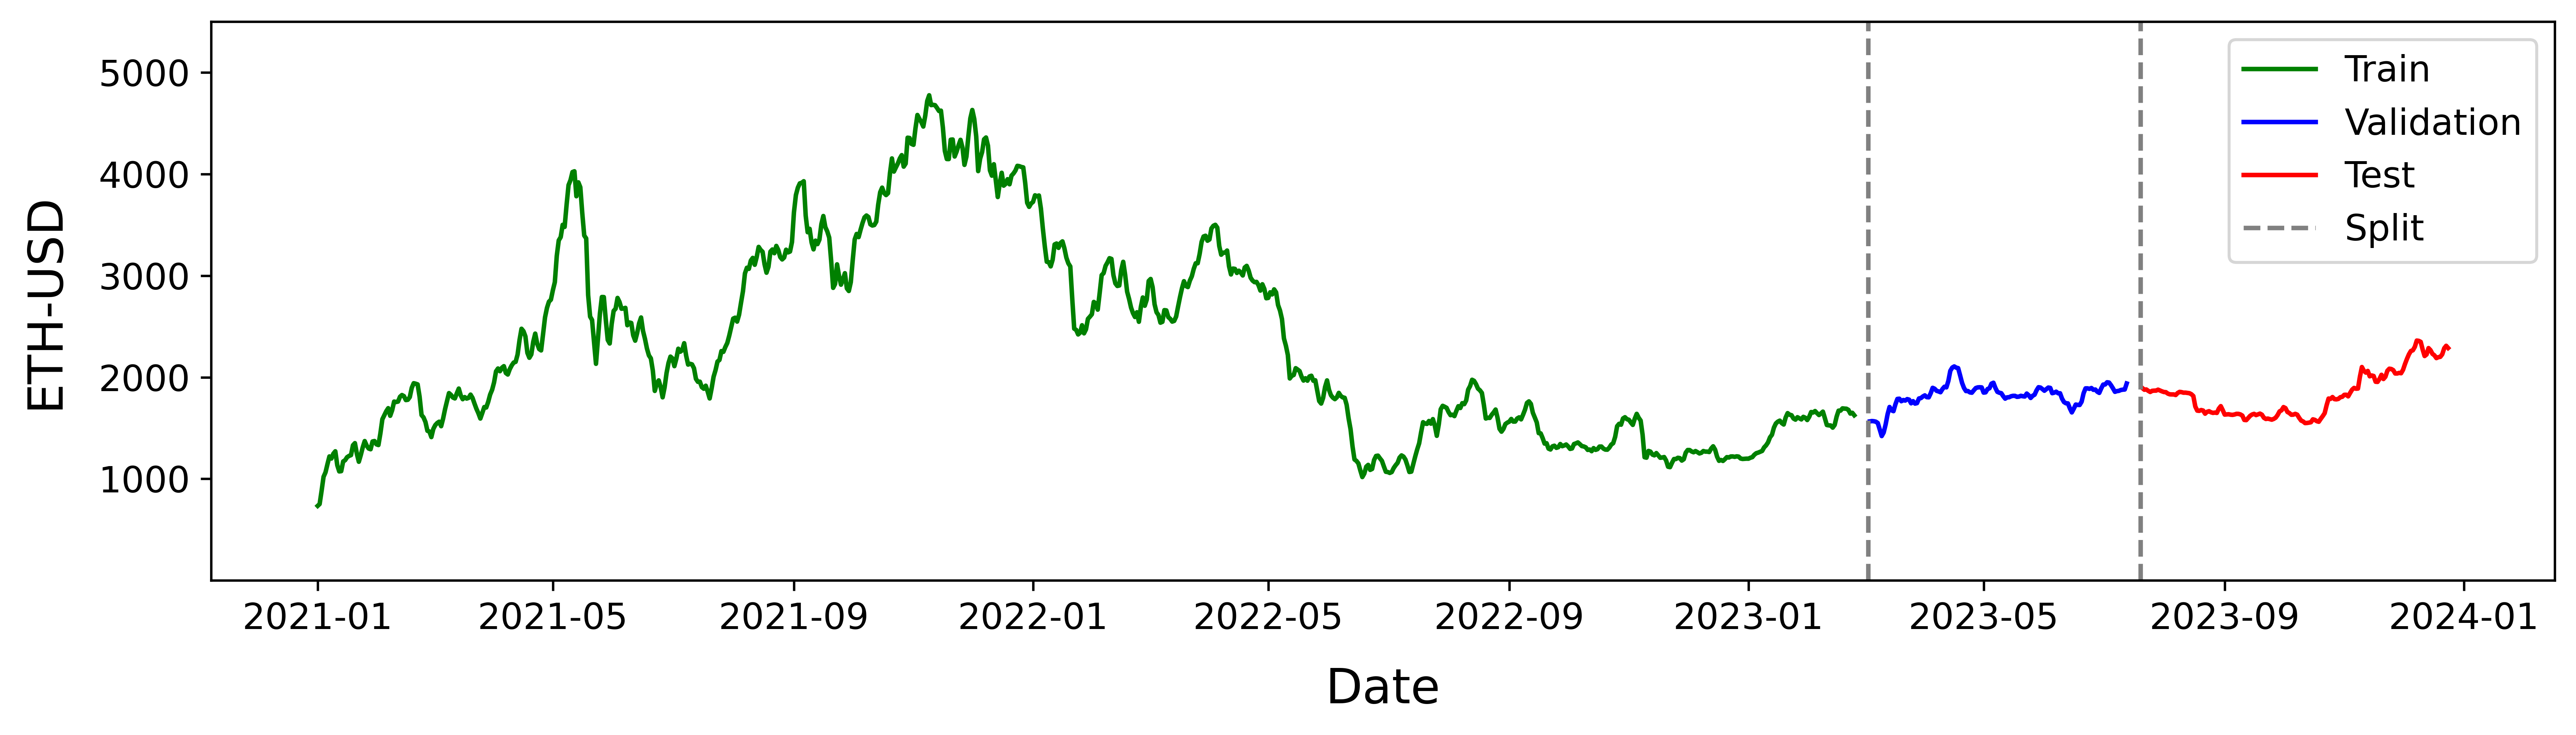
\includegraphics[width=1\linewidth]{figures/test_train_validation.png}
    \caption{Train-Validation-Test split of ETH prices.}
    \label{fig:test_train_validation}
\end{figure}

The nature of price distributions for each split is captured in Figures \ref{fig:kde_distribution} and \ref{fig:splits_classification}. Analysing the Kernel Distribution Estimation (KDE) curves in Figure \ref{fig:kde_distribution}, both the validation and test data have a small, yet identical spread of the rolling 7-day standard deviation of prices. On the other hand, the train data has a much wider spread, which further justifies the choice of using 2021-2023 data as it captures both high and low volatility regions, aiding in the generalisation of the model. Figure \ref{fig:splits_classification} shows that the price movement direction is about even in each split. Comparing this distribution to that of the sentiment analysers in the Figure \ref{fig:sentiment}, FinBERT's distribution is more similar than the other two, possibly suggesting its higher effectiveness in sentiment classification.

\noindent
\begin{minipage}{0.49\textwidth}
    \begin{figure}[H]
        \centering
        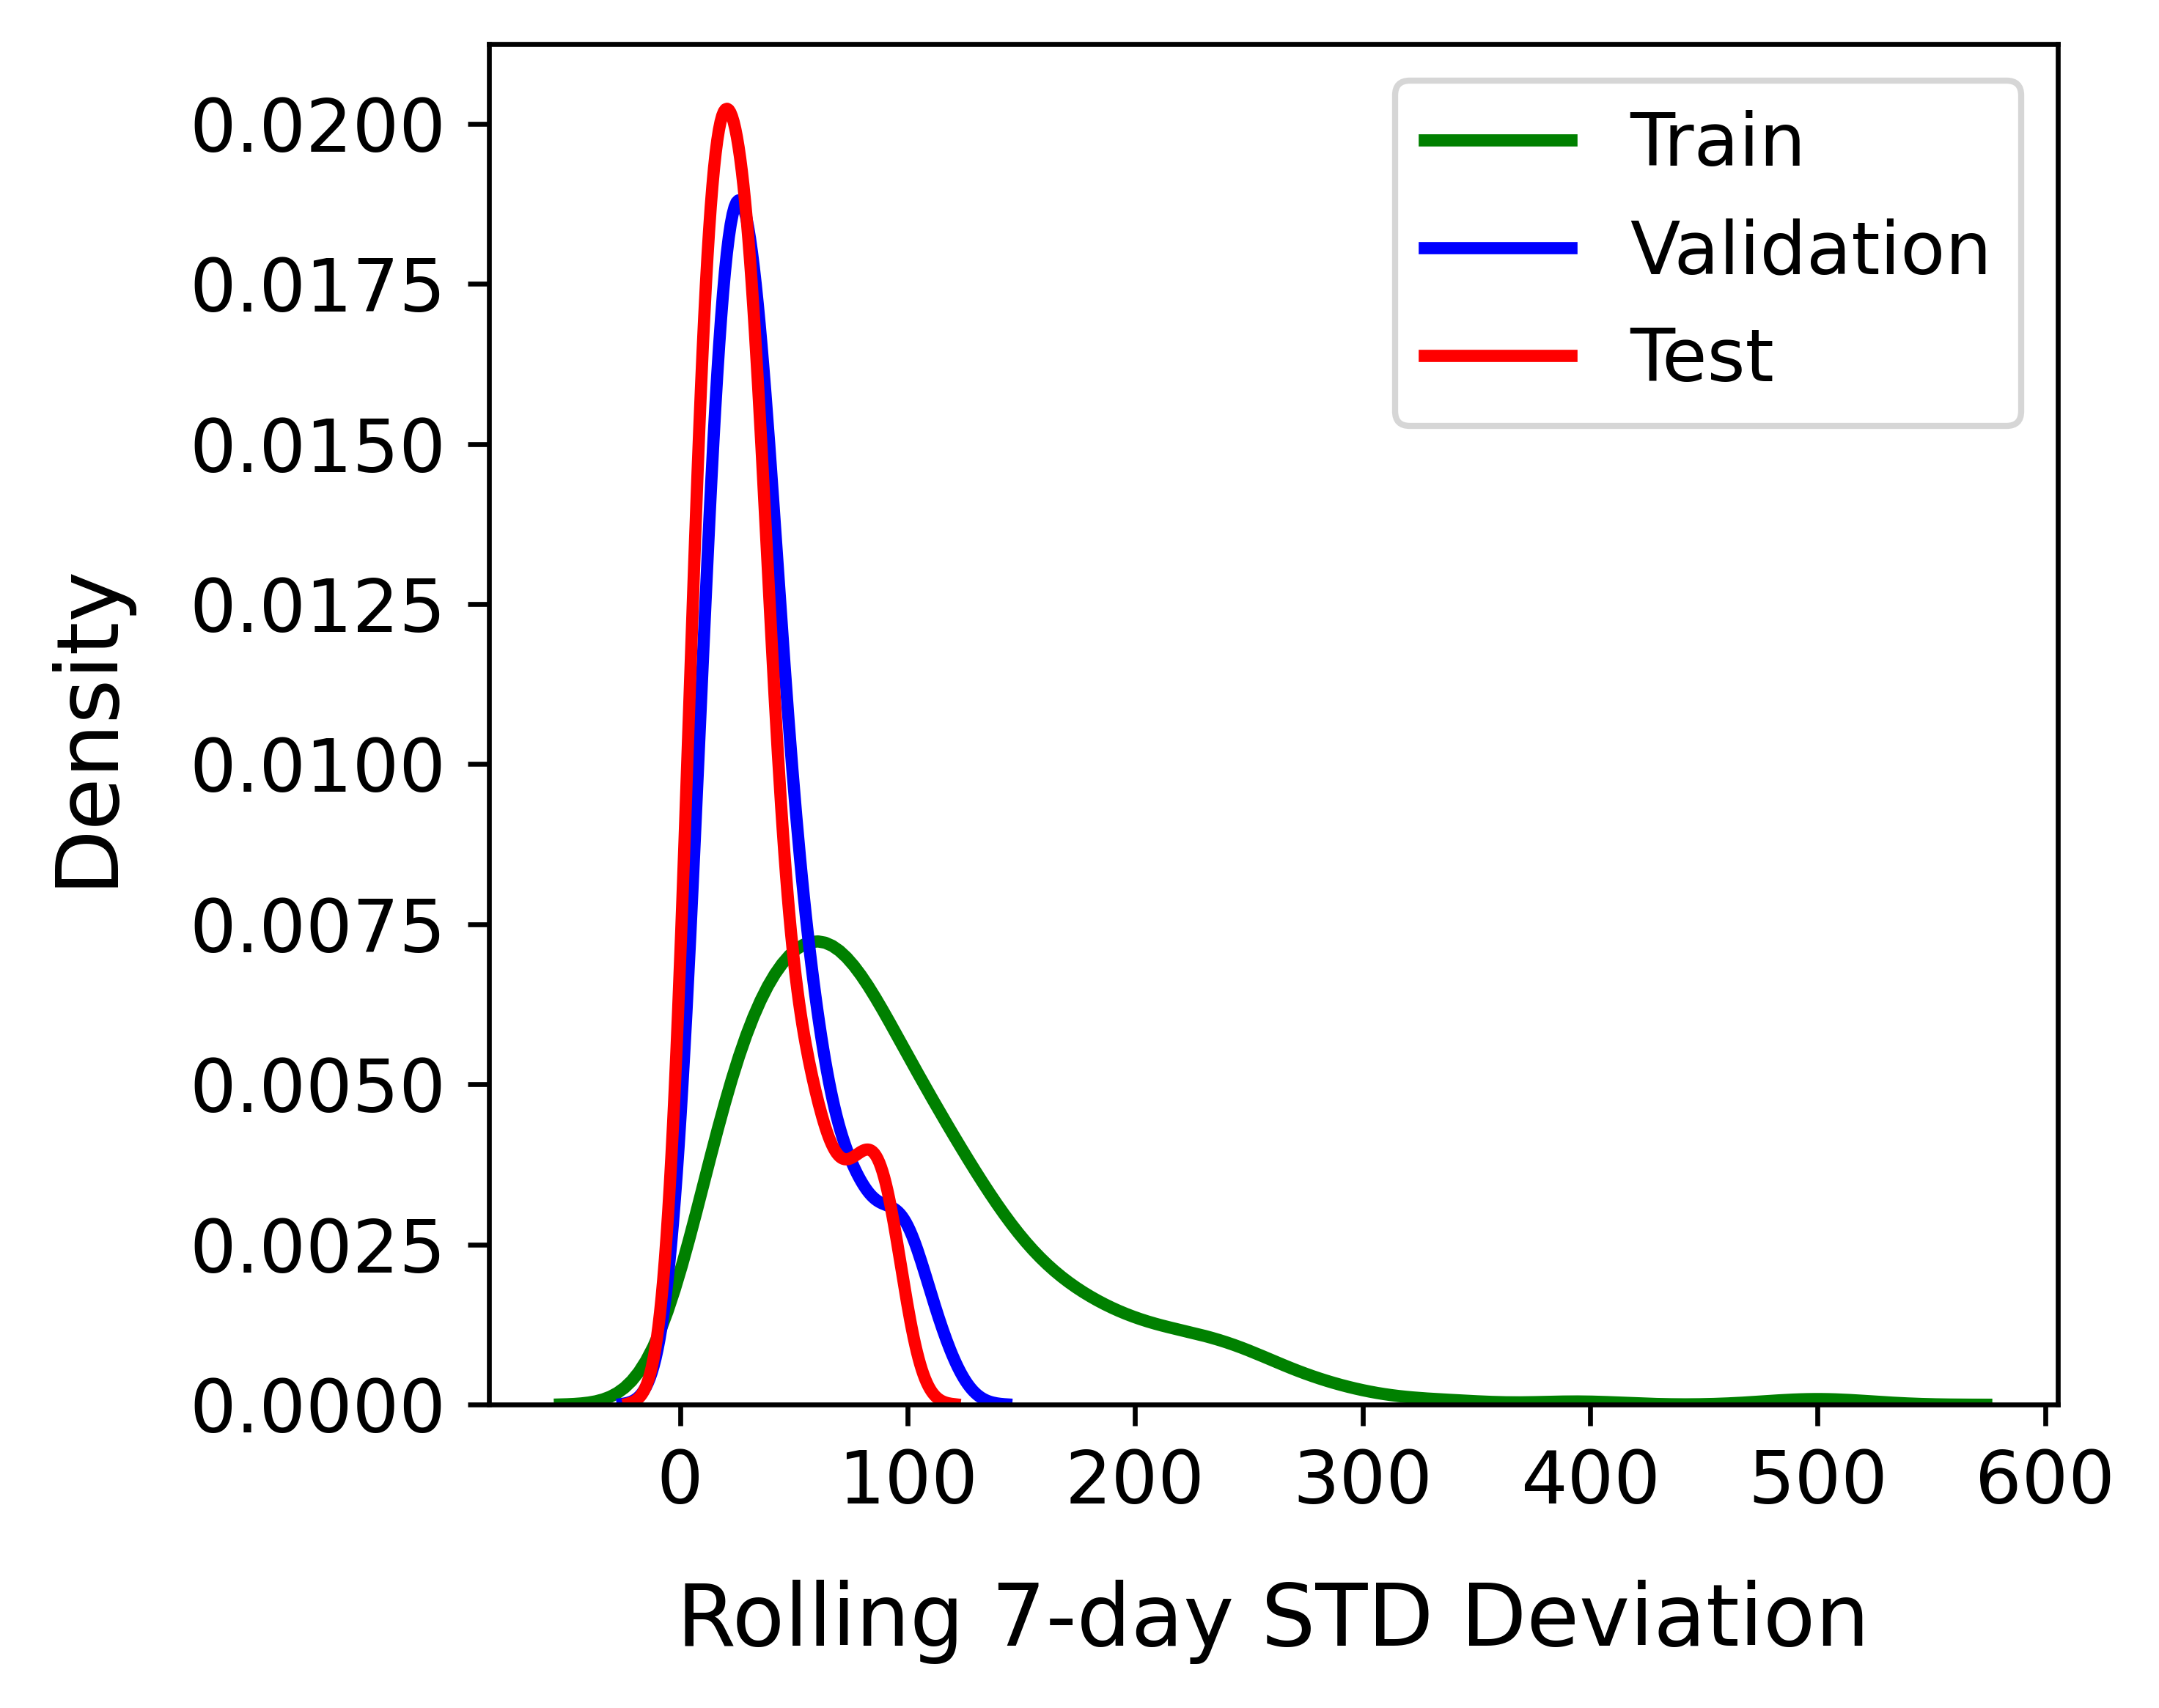
\includegraphics[width=\linewidth]{figures/splits_distribution.png}
        \captionof{figure}{KDE of 7-day rolling STD deviation.}
        \vspace{0.3cm}
        \label{fig:kde_distribution}
    \end{figure}
\end{minipage}
\hfill
\begin{minipage}{0.49\textwidth}
    \begin{figure}[H]
        \centering
        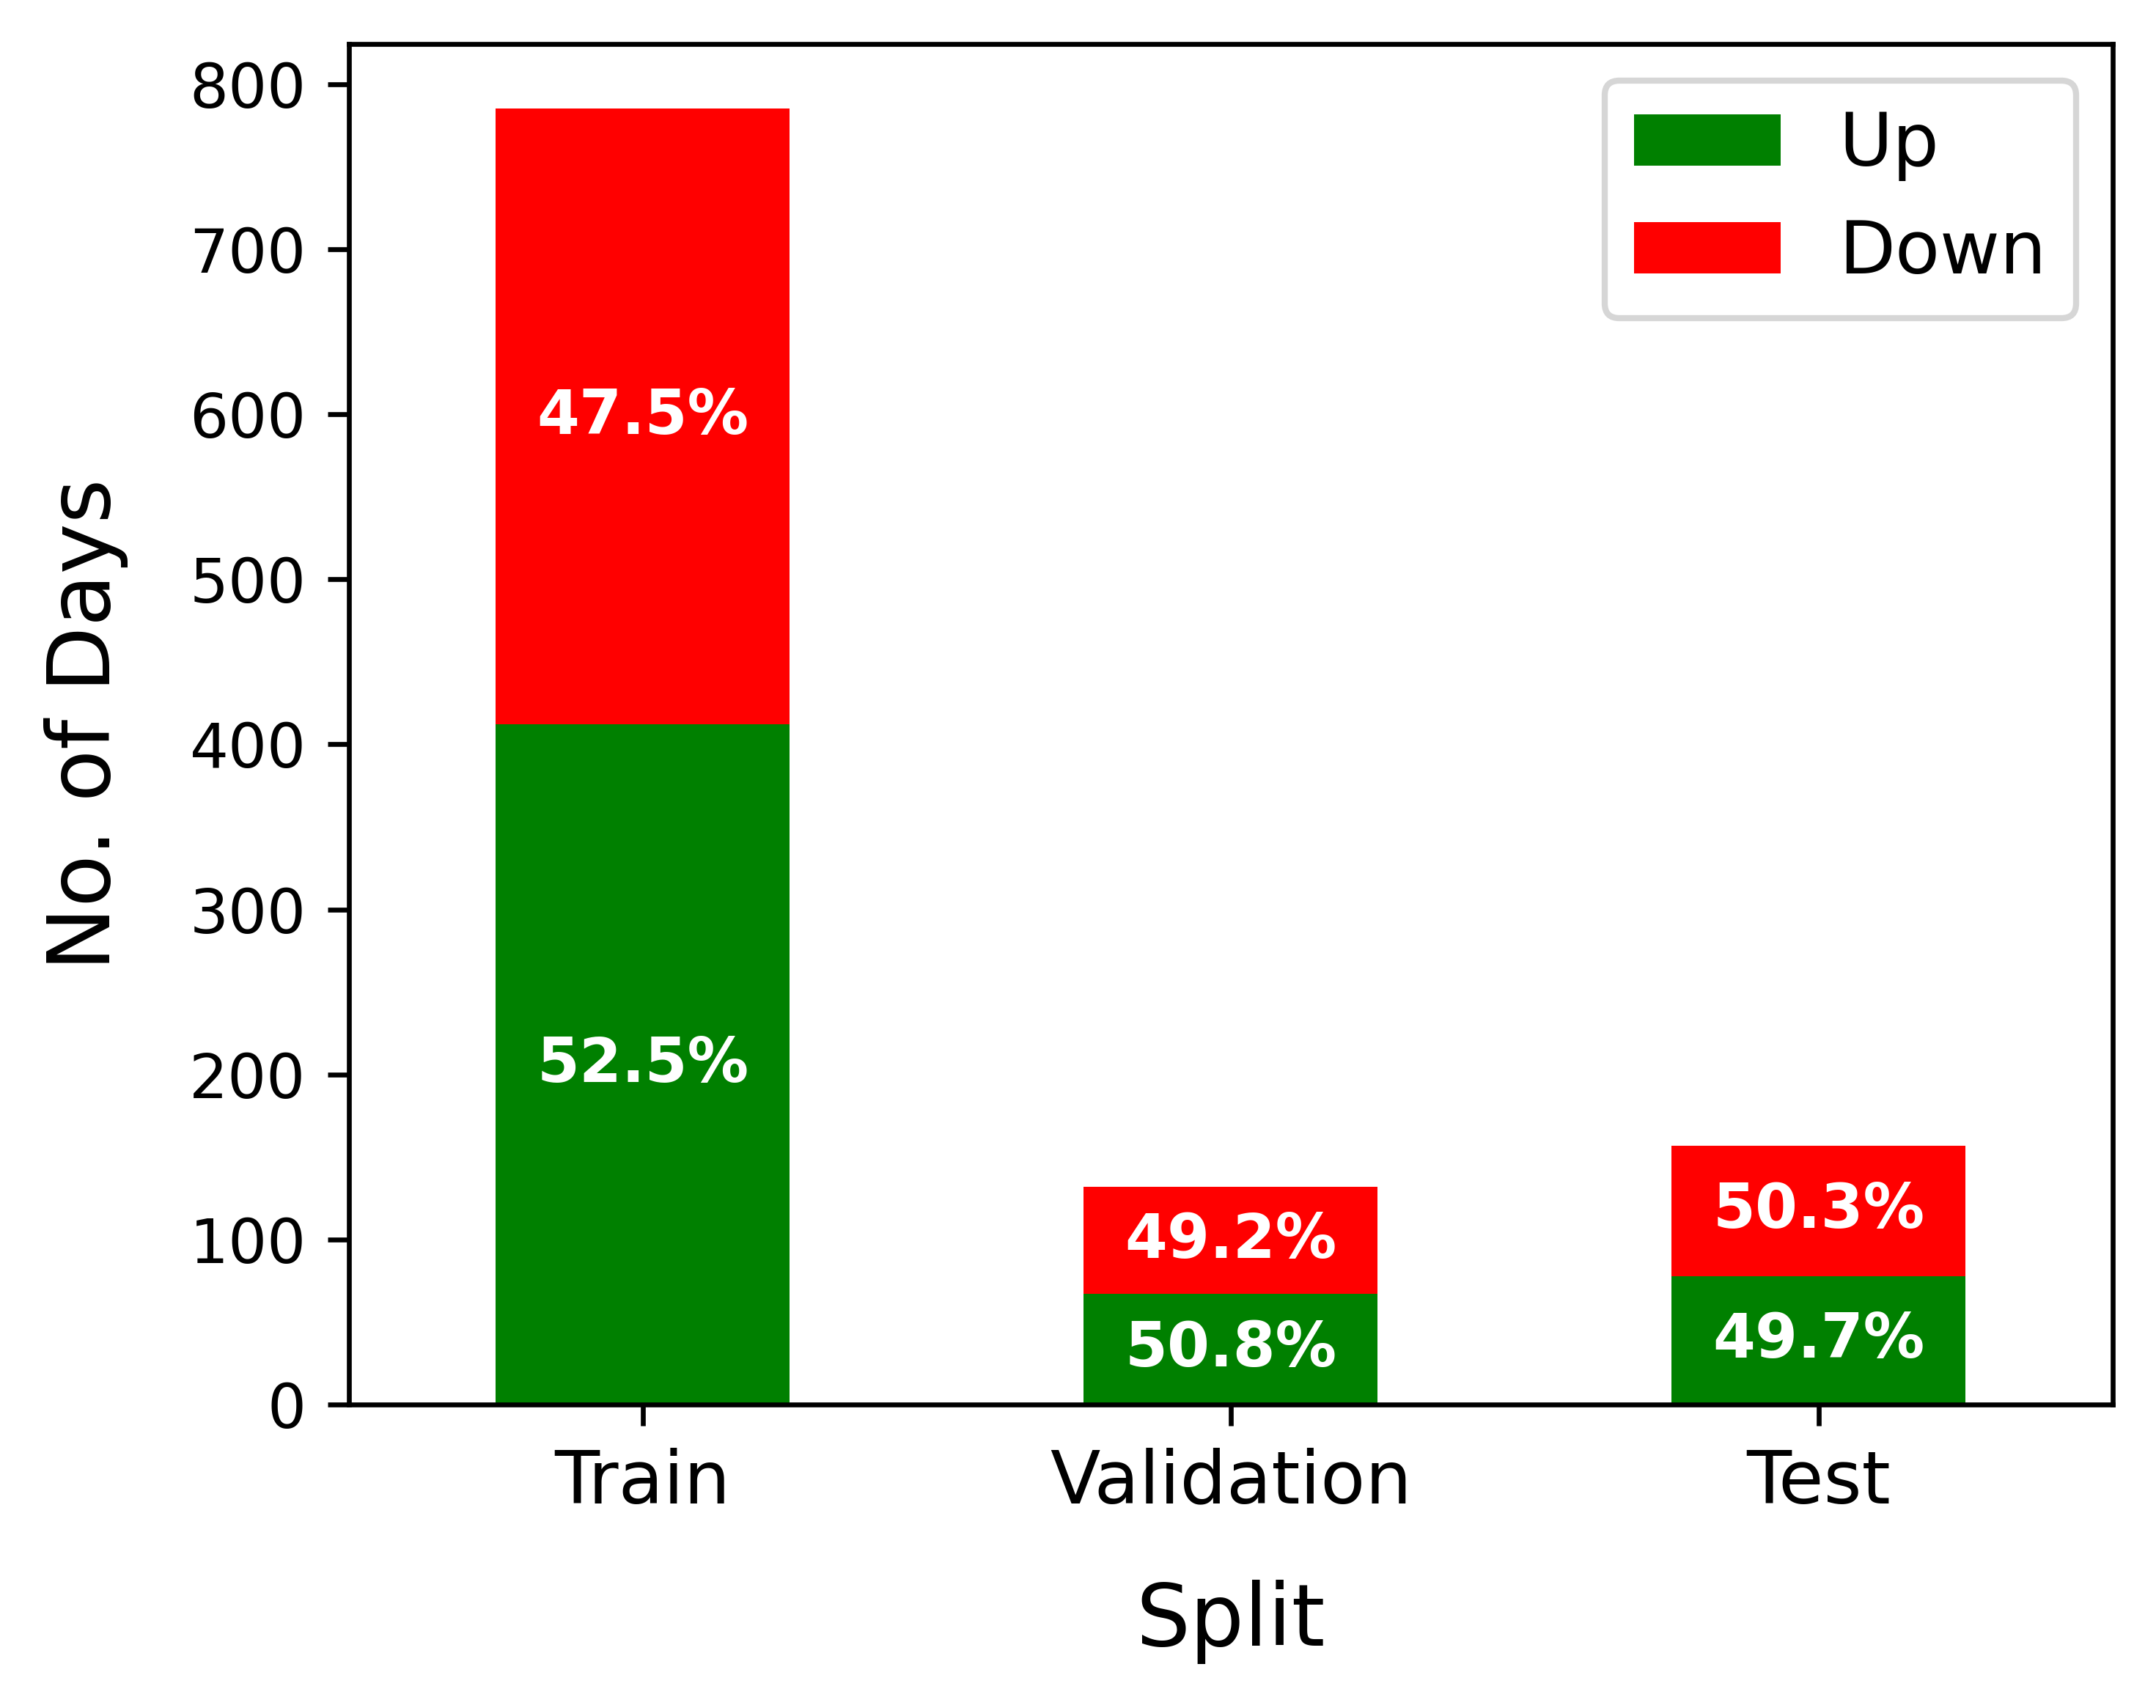
\includegraphics[width=\linewidth]{figures/splits_distribution_classification.png}
        \captionof{figure}{Class distribution of price direction.}
        \vspace{0.3cm}
        \label{fig:splits_classification}
    \end{figure}
\end{minipage} 


\section{Scaling}
% however evaluation will be done on reverse scaling.
Scaling is an important step for deep learning models, and so it was applied as a common step for all models, regardless of whether it was needed or not. The benefit of scaling is that it increases model stability and allows for faster convergence. In this study, a min-max scaling was used to fit and scale the training data, and the same scaler was then used on the validation and the test sets to avoid data leakage. Min-max scaler was chosen as it maintains the distribution of the values. When it comes to evaluating the models, the forecasts were inverse transformed so that the evaluation metrics are meaningful.

\section{Feature Selection}
Feature selection was an important step for blockchain data, given the large number of initial features. However, this filtration step was not performed for the sentiment analysis features since there were only a few. Nevertheless, the results of the feature selection tests are still reported for the sentiment features to gauge their usefulness.

There are various feature selection techniques, but they are broadly categorised into filter, wrapper and embed techniques \cite{theng2024feature}. Whilst filter methods include statistical tests that are independent of the type of ML model, both wrapper and embed methods are model-specific \cite{theng2024feature}. Wrapper methods evaluate features by combining different search strategies with ML training, which allows them to be accurate at the cost of being the most computationally expensive \cite{theng2024feature}. Embed methods utilise model-specific properties, such as feature importances in tree-based models, making them more efficient than wrapper methods while being more accurate than filter methods \cite{theng2024feature}. However, the features selected by the wrapper and embed methods are sensitive to the hyperparameters used; therefore, they depend on hyperparameter tuning. As such, the decision was made to use only filter-based methods to minimise the computational cost and avoid hyperparameter tuning with 33 features. To ensure that the chosen features are correct, multiple filter methods were employed, each using a different approach to quantify correlation.

In this study, three filter methods were used: Spearman's Correlation (SC), Mutual Information (MI) regression and Granger's Causality (GC) test. SC is non-parametric and can capture a monotonic relationship between the target ($y$) and feature ($x$), making it better than Pearson's correlation, which assumes linearity. Equation \ref{eq:spearman_correlation} shows that SC calculates the coefficient ($\rho$) by using the squared difference of ranks (R) across the number of data points (\textit{n}). $\rho$ can range between -1 and 1, indicating both the strength and direction of correlation. Conversely, MI can capture any type of relationship, including non-monotonic relationships. It employs a probabilistic approach using entropy to infer correlation (Equation \ref{eq:mutual_information}) \cite{beraha2019feature}. The values of MI range from 0 to $\infty$; however, to make it easy for comparison, MI scores were min-max scaled. Finally, GC is a statistical test (Equation \ref{eq:grangers_causality}) designed specifically for time series to check if the past values of one time series can forecast values of another \cite{shojaie2022granger}. GC assumes that the time series are stationary \cite{shojaie2022granger}, and so the features were differenced where needed to make them stationary before conducting the test. As per Equation \ref{eq:grangers_causality} \cite{shojaie2022granger}, the maximum number of lags (\textit{p}) to check causality was set to 30 days, where $\tau$ and $\beta$ are coefficients of lags and $\epsilon$ is the error term. This equation shows that GC assumes linearity, when in reality it is not always the case; therefore, GC alone does not suffice. 

\begin{equation}
\label{eq:spearman_correlation}
\rho = 1 - \frac{6 \sum_{i=1}^{n} (R(x_i)-R(y_i))^2}{n(n^2 - 1)}
\end{equation}

\begin{equation}
\label{eq:mutual_information}
I(X; Y) = H(Y) - H(Y|X)
% I(X; Y) = \int_{Y} \int_{X} p(x, y) \log \left( \frac{p(x, y)}{p(x)\, p(y)} \right) \, dx \, dy
\end{equation}

\begin{equation}
\label{eq:grangers_causality}
y_t = \sum_{i=1}^p \tau_i y_{t-i} + \sum_{j=1}^p \beta_j x_{t-j} + \varepsilon_t \\
\end{equation}

The results of the test are summarised in Tables \ref{tab:feature_selection_blockchain} and \ref{tab:feature_selection_sentiment} for blockchain data and news headline sentiment, respectively. The value recorded for SC is $\rho$, where any moderate or stronger (greater than or equal to 0.3) coefficients are highlighted in bold \cite{rovetta2020raiders}. For MI, it is the min-max scaled scores, and the top 10 values across all features from all coins are highlighted in bold. For GC, it is the total number of lags\footnote{Lags are not consecutive, e.g. 3 could mean lags 1,4 and 20 are causal.} out of 30 days that show causality. Note that the table omits values for ETH Average Price, given that it is a baseline feature. The features of the blockchain data that are significant in at least 2 or more of these tests were directly selected. The only two features that were additionally selected were ETH Total Volume and BTC Average Transaction Fees. Both were added because their SC coefficient is very close to the 0.3 threshold, and GC shows a significant number of lags. Based on this feature selection step, more than half the features were removed, leaving only 14 blockchain features. The features selected are highlighted in bold in Table \ref{tab:feature_selection_blockchain} with superscript initials to refer to the coins.

While Table \ref{tab:feature_selection_blockchain} only reported the values against the target ETH Average Price, Table \ref{tab:feature_selection_sentiment} also includes ETH Average Price Direction, given that the sentiment label is also a categorical feature. Regardless of the target, both SC and MI values are very low. Though the average sentiment scores of the different models show very weak correlation, the sentiment label is more useful, which further justifies the decision of using it, as made in Section \ref{sec:data_partitioning}. From an initial comparison across the tests for all sentiment models, it is clear that FinBERT shows the strongest correlation.

% \newcolumntype{C}[1]{>{\centering\arraybackslash}p{#1}}
\begin{table}[H]
\centering
\caption{Blockchain feature selection test results.}
\label{tab:feature_selection_blockchain}
\begin{adjustbox}{max width=\textwidth}
\begin{threeparttable}
\begin{tabular}{p{5cm} C{1cm} C{1cm} C{1cm} | C{1cm} C{1cm} C{1cm} | C{1cm} C{1cm} C{1cm}}
\toprule
\textbf{\raggedright Feature} & \multicolumn{3}{c}{\textbf{ETH}} & \multicolumn{3}{c}{\textbf{BTC}} & \multicolumn{3}{c}{\textbf{LTC}}\\
\cmidrule(lr){2-10}
 & \textbf{SC} & \textbf{MI} & \textbf{GC} & \textbf{SC} & \textbf{MI} & \textbf{GC} & \textbf{SC} & \textbf{MI} & \textbf{GC}\\
\midrule
% Sample rows
\raggedright \textbf{Average Price}\textsuperscript{EBL} & -& - & - & \textbf{0.81}& \textbf{1}& \textbf{10}& \textbf{0.69}& \textbf{0.75}& \textbf{21} \\
\raggedright \textbf{Total Volume}\textsuperscript{EL} & 0.29& 0.10& \textbf{27} & 0.11& 0.06& 0& \textbf{0.42}& 0.20& \textbf{16} \\
\raggedright On-chain Transaction Count & \textbf{0.47}& 0.15& 0 & -0.14& 0.12& 0& \textbf{0.52}& 0.21& 0 \\
\raggedright \textbf{Average Transaction Fees}\textsuperscript{EB} & \textbf{0.77}& \textbf{0.38}& \textbf{20} & -0.27& 0.16& \textbf{5}& -0.12& 0.11& 0 \\
\raggedright Active Addresses & \textbf{0.52}& 0.15& 0 & 0.04& 0.01& \textbf{10}& \textbf{0.63}& 0.19& 0\\
\raggedright Average Block Size & -0.04& \textbf{0.39}& 0 & -0.19& 0.15& 0& \textbf{0.45}& 0.10& 0\\
\raggedright \textbf{Difficulty}\textsuperscript{BL} & -& -& - & \textbf{-0.47}& \textbf{0.86}& \textbf{5}& \textbf{-0.35}& \textbf{0.69}& 0\\
\raggedright \textbf{Average Block Time}\textsuperscript{E}&\textbf{0.49}& \textbf{0.31}& 0 & -& -& -& -& -& -\\
\raggedright Gas Limit & 0.26& 0.18&\textbf{1} & -& -& -& -& -& -\\
\raggedright \textbf{Gas Used}\textsuperscript{E}  & -0.24& \textbf{0.50}&\textbf{8} & -& -& -& -& -& -\\
\raggedright \textbf{Average Gas Price}\textsuperscript{E} & \textbf{0.52}& 0.22&\textbf{20} & -& -& -& -& -& -\\
\raggedright Deployed Contracts & -0.09& 0.09&\textbf{2} & -& -& -& -& -& -\\
\raggedright Verified Contracts & \textbf{-0.42}& 0.25&0 & -& -& -& -& -& -\\
\raggedright New Addresses & 0.10& 0.18& 0 & -0.09& 0.03& 0& \textbf{0.46}& 0.21& 0\\
\raggedright On-chain Transaction Volume & 0.10& 0& \textbf{28} & 0.06& 0.08& \textbf{25}& -& -& -\\
\raggedright \textbf{Hashrate\textsuperscript{BL}} & -& -& - & \textbf{-0.43}& \textbf{0.36}& 0& \textbf{-0.35}& \textbf{0.46}& 0\\
% Add more rows as needed
\bottomrule
\end{tabular}
\vspace{0.5em}
\begin{tablenotes}
\footnotesize
\item[E] Feature selected for ETH.
\item[B] Feature selected for BTC.
\item[L] Feature selected for LTC.
\end{tablenotes}
\end{threeparttable}
\end{adjustbox}
\end{table}

\begin{table}[H]
\centering
\caption{Sentiment feature selection test results.}
\vspace{-0.35cm}
\label{tab:feature_selection_sentiment}
\begin{adjustbox}{max width=\textwidth}
\begin{tabular}{p{5.5cm} p{5.5cm} C{1cm} C{1cm} C{1cm}}\\
\toprule
\textbf{\raggedright Target} &
\textbf{\raggedright Feature} & \textbf{\raggedright SC} & \textbf{\raggedright MI} & \textbf{\raggedright GC}\\
\midrule
\multirow{3}{*}{\textbf{ETH Average Price}} & \textbf{VADER Average Score} & 0.14 & 0.03 & \textbf{3} \\
& \textbf{FinBERT Average Score} & 0.19 & 0 & \textbf{1} \\
& \textbf{CryptoBERT Average Score} & 0.11 & 0 & 0 \\
\hline
\multirow{3}{*}{\textbf{ETH Average Price Direction}} & \textbf{VADER Sentiment Label} & 0.09 & 0 & \textbf{3} \\
& \textbf{FinBERT Sentiment Label} & 0.25 & 0 & \textbf{30} \\
& \textbf{CryptoBERT Sentiment Label} & 0.07 & 0 & 0 \\
\bottomrule
\end{tabular}
\end{adjustbox}
\end{table}

\section{Model Training}
\label{model_training}
To train and evaluate the model, a cross-validation strategy was used along with hyperparameter tuning to find the best baseline model (includes lagged prices only). The effects of the selected features were then assessed by stepwise addition of each set of selected features (ETH blockchain data, BTC blockchain data, LTC blockchain data, sentiment analysis scores/labels). 

\subsection{Cross Validation}
Cross validation of time series is different to other datasets in that temporal order must be maintained to avoid data leakage. As such, a rolling forecast origin approach was employed with a one-day step forward, essentially creating multiple test periods within the time frame of the validation data to allow for a more accurate mean of the evaluation metrics \cite{hewamalage2023forecast}. The rolling approach was done using a sliding window, where $x$, the (past) input features, slides forward by one day as new data becomes available. Figure \ref{fig:cv} is a visual example of the cross-validation approach where the input window size is a parameter to be tuned.

For ARIMA only, the model was refitted with all of the past data (expanding training set) whilst moving forward due to reasons mentioned in Section \ref{sec:statistical_models}. Although refitting is also important for ML models, it is done less frequently because it can be computationally expensive to retrain as soon as new data is available \cite{hewamalage2023forecast}. Typically, models are only retrained when concept drift is apparent \cite{hewamalage2023forecast}. However, given that the test set is small, retraining was an unnecessary computational overhead, and so ML models had a fixed training set.

\begin{figure} [H]
    \centering
    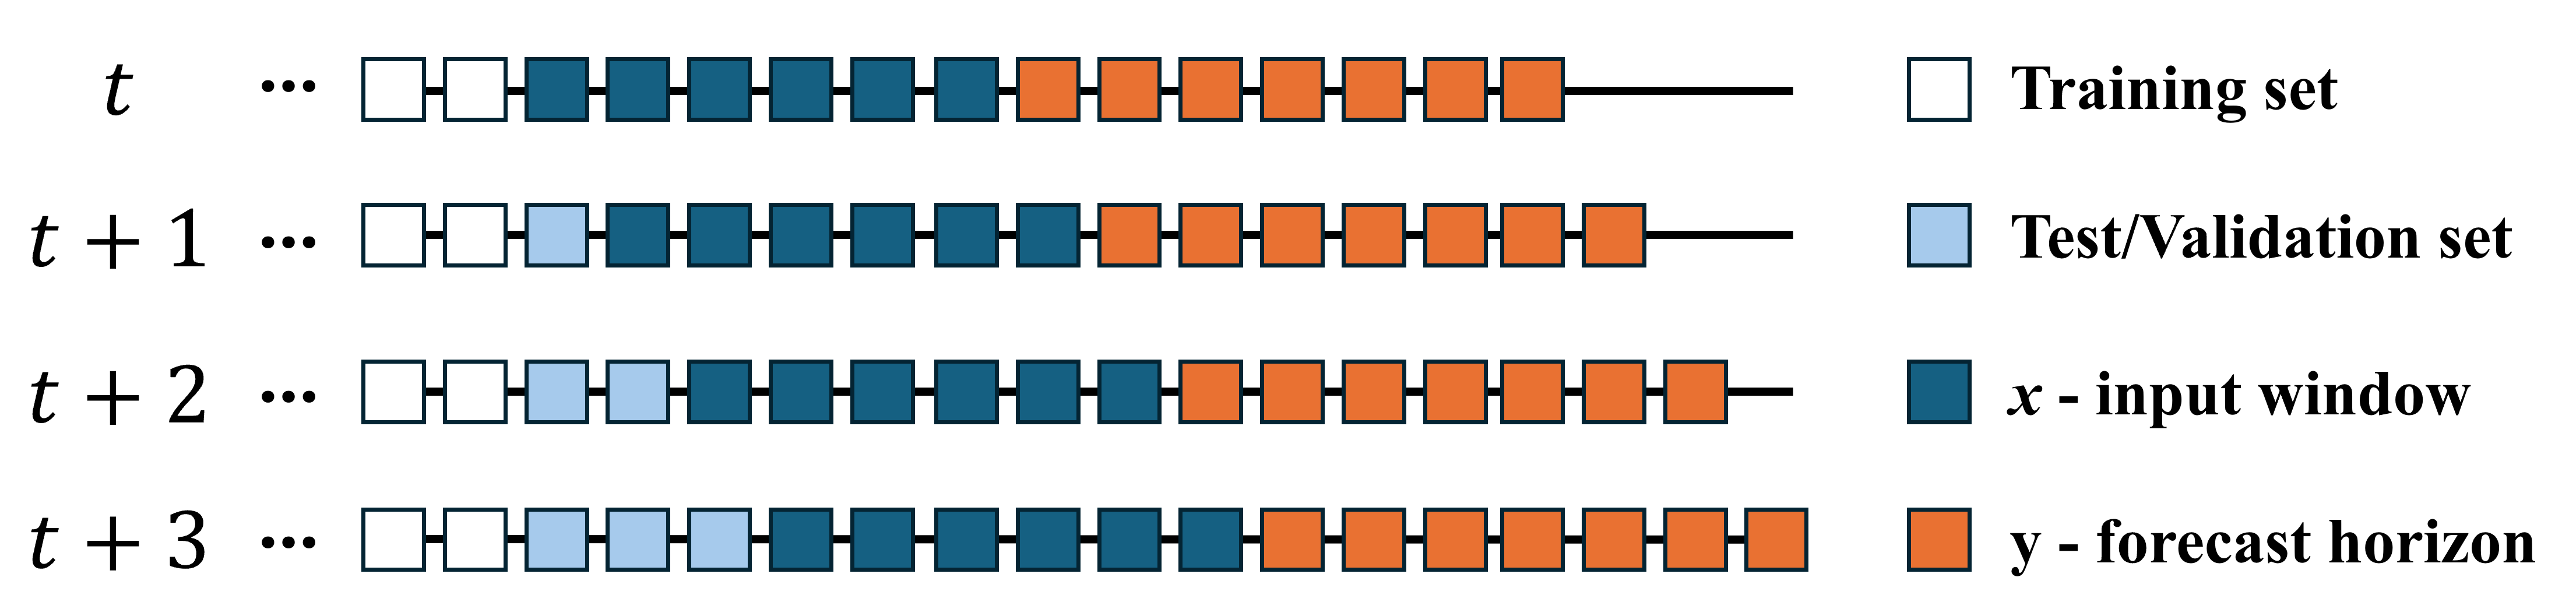
\includegraphics[width=0.75\linewidth]{figures/cv.png}
    \caption{Diagramatic example of sliding-window rolling-origin cross-validation approach.}
    \label{fig:cv}
\end{figure}

\subsection{Models}
An ARIMA model was used as the statistical baseline, and three machine learning models were subsequently investigated in this study. All models were configured for multi-output so that the entire 7-day horizon was output together. Multi-output allows the model to learn and exploit dependencies across time steps in a single training process, improving coherence and reducing computational overhead compared to training separate models for each forecasted day. In the sections below, each model and its relevant hyperparameters are explained to provide a high-level understanding.

\subsubsection{ARIMA}
ARIMA model is defined by three components \cite{sailaja2024crypto}: 
\begin{itemize}
    \item \textbf{Autoregression} (AR) makes use of the past values to predict the future values ($y_t$). This is defined by \textit{p} parameter, where higher values mean greater reliance on previous values.
    \item \textbf{Integration} (I) defines the order of differencing (\textit{d}) needed for stationarity.
    \item \textbf{Moving average} (MA) - the sum of past error terms. This is defined by \textit{q} parameter, where higher values mean greater reliance on previous error terms ($\epsilon$).
\end{itemize}
The above is summarised by Equation \ref{eq:arima} \cite{pyflux_arima}, where $\phi$ and $\theta$ are fitted coefficients for \textit{p} and \textit{q} terms respectively.
\begin{equation}
\label{eq:arima}
y_t^{(d)} = \sum_{i=1}^{p} \phi_i y_{t-i}^{(d)} + \sum_{j=1}^{q} \theta_j \epsilon_{t-j}+ \epsilon_t 
\end{equation}

The value \textit{d} was already established as 1 from Section \ref{sec:eda}. \textit{p} can be speculated from the PACF graph in Figure \ref{fig:pacf}, which can be a maximum value of 7, so all values from 1 to 7 were tested. \textit{q} can be speculated from the ACF graph in Figure \ref{fig:acf}, which only has a spike at lag 1, and so there was no other exploration to be done for \textit{q}.

\subsubsection{XGBoost}
XGBoost works similarly to GBM in that it iteratively corrects the errors (residuals) made by the previous weak learner (tree), and the final prediction is the sum of outputs of each learner \cite{chen2016xgboost}, as illustrated in Figure \ref{fig:xgboost}. What differentiates XGBoost from GBM is its improvement in performance and speed. XGBoost has the addition of L1 ($\alpha$) and L2 ($\lambda$) regularisation \cite{xgboost_parameters}, which can minimise certain feature weights to zero and evenly reduce the weights for all features, respectively. Both regularisation techniques give finer control to tune the model for generalisation. XGBoost also has parallelisation capability, allowing for much faster training \cite{chen2016xgboost}. In addition to the typical hyperparameters for tree-based ML models, such as the number of trees ($N_{est}$), there is also gamma ($\gamma$), which is a threshold for the minimum loss reduction required for further splitting of a leaf node \cite{xgboost_parameters}. A larger $\gamma$ will produce shallower trees, which is useful to reduce overfitting. 

\begin{figure}
    \centering
    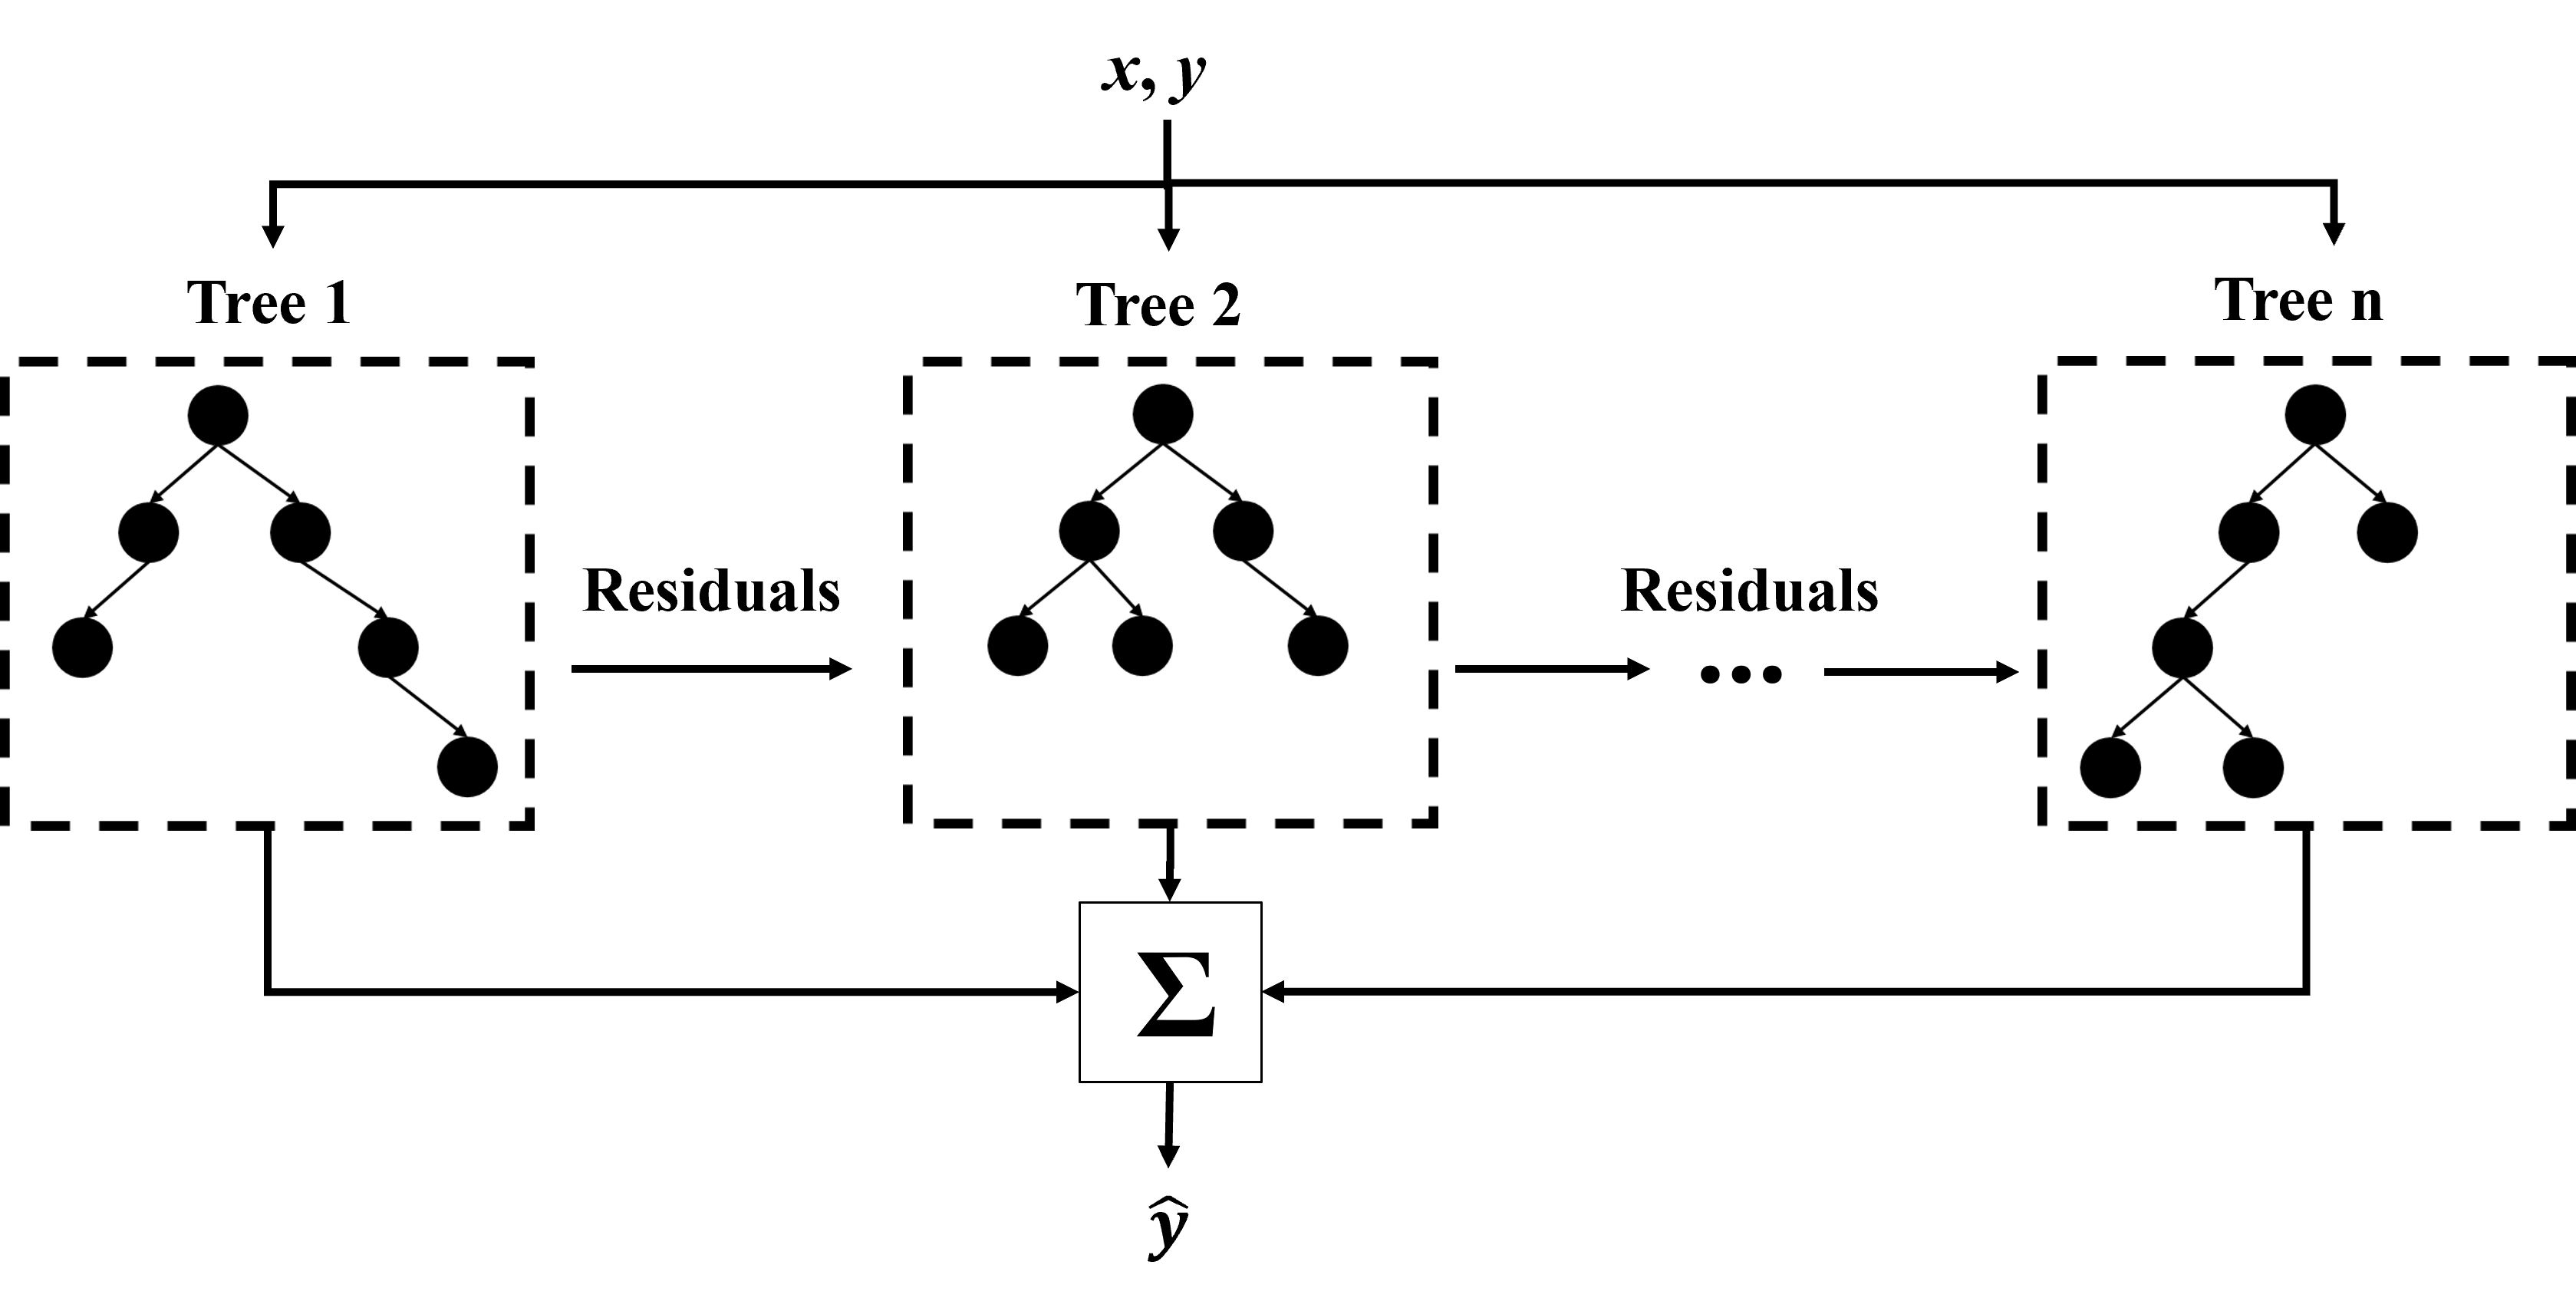
\includegraphics[width=0.8\linewidth]{figures/xgboost.png}
    \caption{XGBoost architectural diagram.}
    \label{fig:xgboost}
\end{figure}

\subsubsection{BiGRU}
The choice of using GRU over LSTM was because the ACF and PACF graphs show short-term dependencies; therefore, the use of a more computationally efficient model over better long-term memory is ideal. A GRU cell only has two gates, update and reset \cite{mazinani2025deep}, as shown in the detailed view of a GRU cell in Figure \ref{fig:bi-gru}. The update ($u$) gate determines the amount of past information ($h_{t-1}$) that must be passed to the next cell \cite{mazinani2025deep}. The reset ($r$) gate determines the amount of past information that must be removed \cite{mazinani2025deep}. The operations within these gates are highlighted by the set of equations below \cite{mazinani2025deep}, where $W$, $V$ and $b$ are weight and bias matrices that are learned during training, and $\tilde{h}_t$ is the proposed hidden state. 

\begin{equation}
\label{eq:update_gate}
    u_t = \sigma(W_u x_t + V_u h_{t-1} + b_z)
\end{equation}
\begin{equation}
\label{eq:reset_gate}
    r_t = \sigma(W_r x_t + V_r h_{t-1} + b_r)
\end{equation}
\begin{equation}
\label{eq:candidate_hidden_state}
    \tilde{h}_t = \tanh(W_h x_t + V_h (r_t \odot h_{t-1}) + b_h)
\end{equation}
\begin{equation}
\label{eq:new_hidden_state}
    h_t = (1 - u_t) \odot {h}_{t-1} + u_t \odot \tilde{h}_t
\end{equation}

\begin{figure}[H]
    \centering
    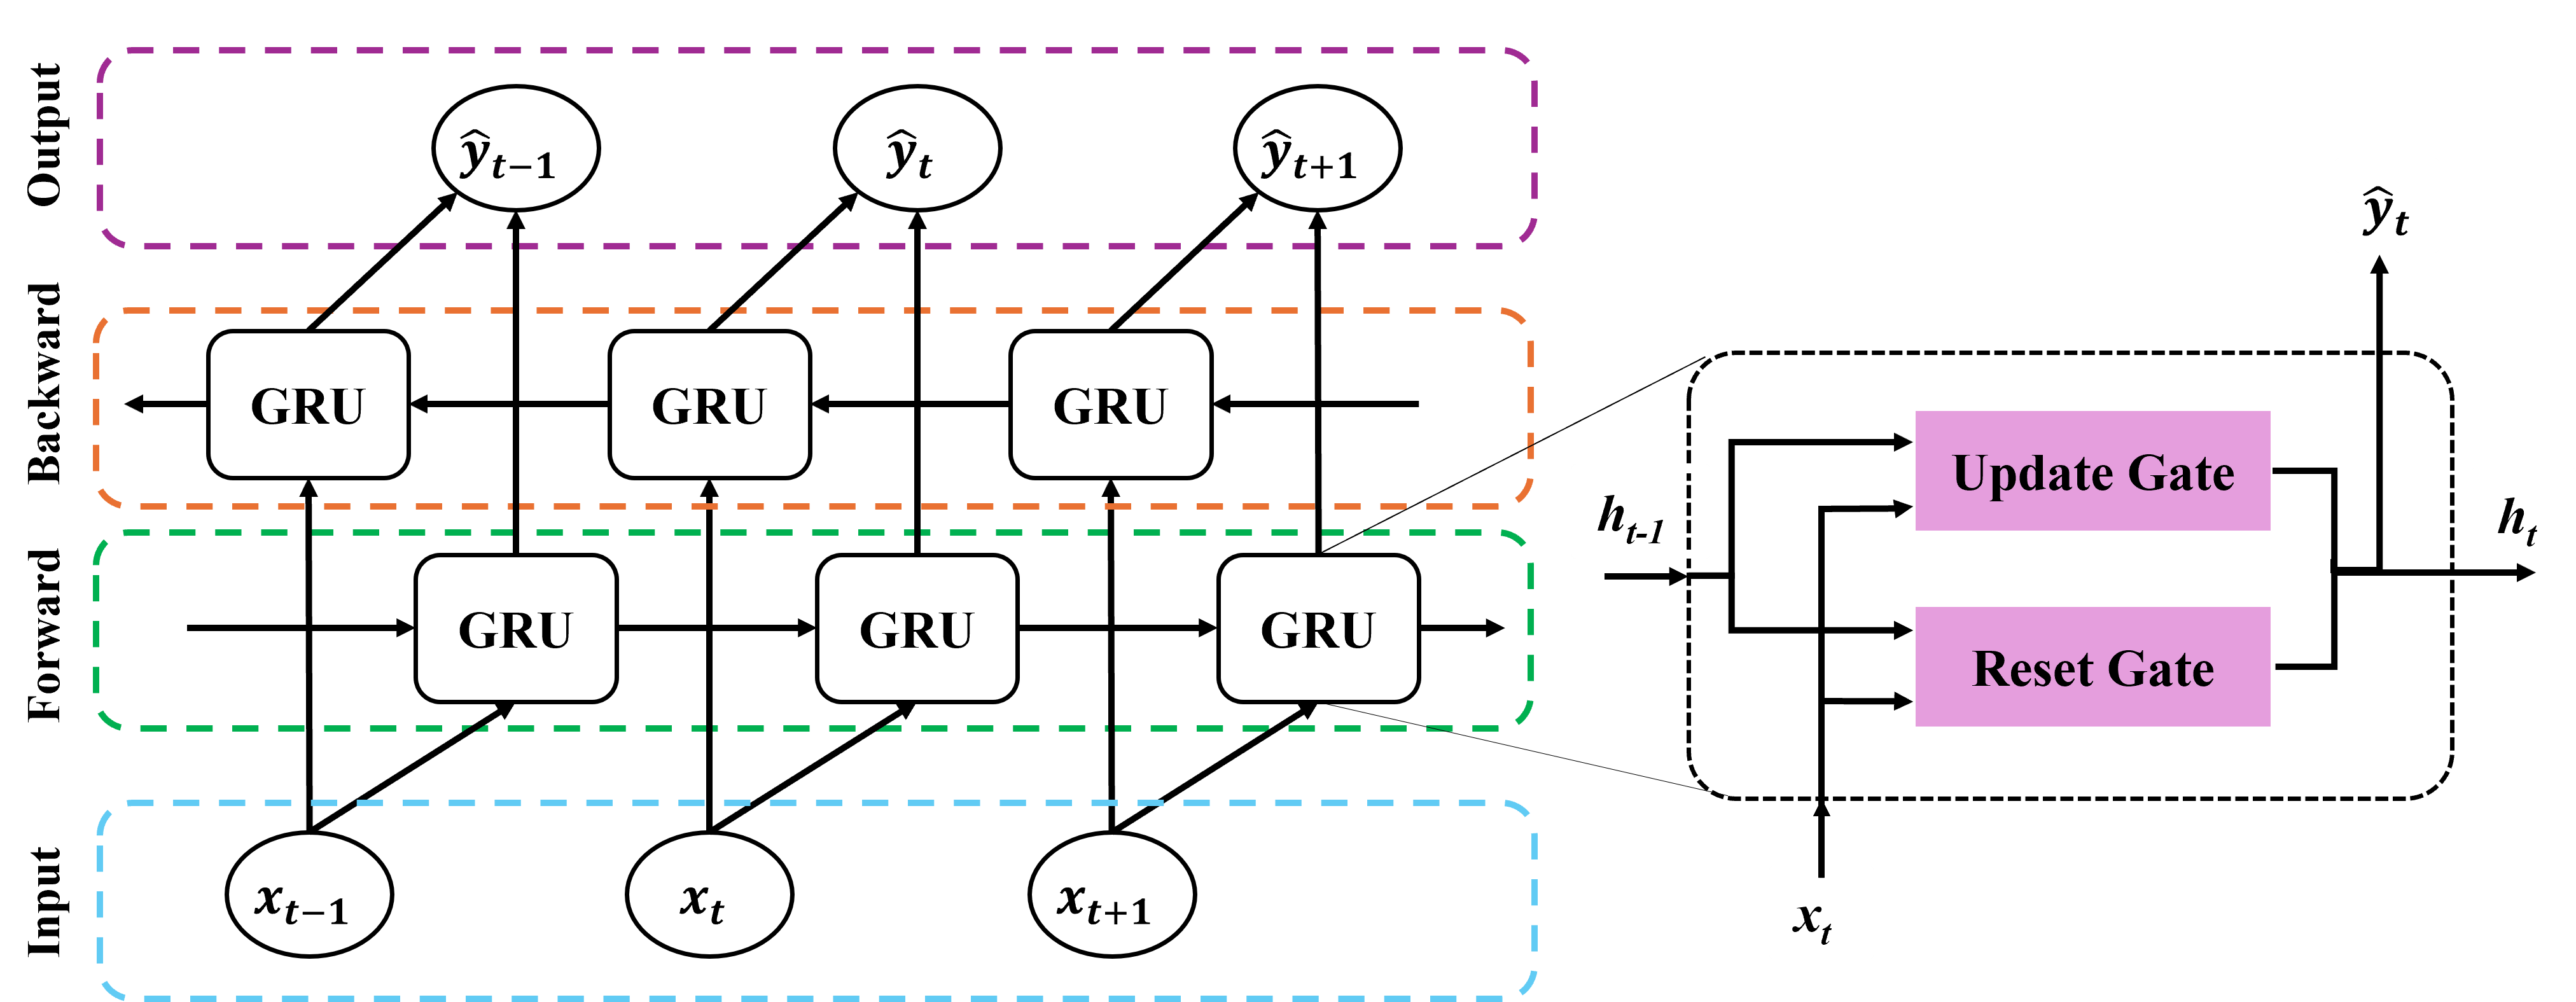
\includegraphics[width=1\linewidth]{figures/bi-gru.png}
    \caption{BiGRU architectural diagram.}
    \label{fig:bi-gru}
\end{figure}

The key hyperparameters to tune with the BiGRU model are the number of bidirectional layers ($N_{BiGRU}$), the number of GRU cells (U) in each, learning rate ($\eta$), dropout (D) and the number of epochs (E) to train.

\subsubsection{1DCNN-BiGRU}
To analyse the effect of CNN layers preceding BiGRU, the hybrid of the two, CNN-BiGRU, is a good candidate for experimentation. Given the understanding of how GRU works, CNN will be explained in this section. In this study, a one-dimensional (1D) CNN was used as it is ideal for sequential data \cite{hoa2025hybrid}. There are two main components of 1DCNN: the convolution layer and the pooling layer \cite{mazinani2025deep}. 

The convolution layer uses a kernel\footnote{A kernel is a sliding window, which needs to be smaller than the length of the input sequence \textit{x}.} \textit{w} of size \textit{k} to produce a feature map \textit{m}. Equation \ref{eq:1dcnn} defines the convolution process \cite{hoa2025hybrid}, where the input \textit{x} at time step \textit{t} is multiplied by the kernel weights \textit{w}, and \textit{b} is the bias term. However, a single 1DCNN layer can have multiple kernels, each with the capability of learning different patterns. The number of kernels is defined by the filters ($N_{filters}$) hyperparameter. 

\begin{equation}
\label{eq:1dcnn}
m[t] = \sum_{i=0}^{k-1} w[i] \cdot x[t + i] + b
\end{equation}

The pooling layer is an optional layer that is used after a convolution layer for downsampling, which reduces the overall dimension of the feature map, hence reducing computational complexity \cite{zhao2024improved}. There are two main types of pooling: max pooling and average pooling \cite{zhao2024improved}. Max pooling takes the maximum value in the pool window ($P_{max}$), and is ideal for capturing dominant local (short-term) features such as spikes and outliers \cite{zhao2024improved}. Average pooling takes the average value, essentially smoothing the result, making it better for capturing long-term trends \cite{zhao2024improved}. Given GRU is better at capturing long-term dependencies, using max pooling would be more appropriate, as shown by the study \cite{mazinani2025deep}. Regardless of the pooling type, both have pooling size as a key hyperparameter, which essentially dictates the window size for the pooling operation. Another way of downsampling is by controlling the stride length taken by the kernel; however, this was kept at a stride length of 1 to preserve the short-term temporal resolution. 

\subsection{Hyperparameter Tuning}
Grid search was used for hyperparameter tuning because it is transparent and deterministic. Although it is exhaustive and can be computationally expensive for more complex ML models, it still provides straightforward control over the search space. Table \ref{tab:gridsearch_space} shows the grid search space for each ML model that was explored for each combination of feature sets in Table \ref{tab:feature_set_models}. For ARIMA and XGBoost, a large combination was explored, as the training time of a singular model was sub-second. For 1DCNN-BiGRU, the best hyperparameters of the BiGRU model for each feature set were kept, and only the CNN architecture preceding it was experimented with. This not only reduced the number of experiments but also provided a controlled way to investigate whether 1DCNN was effective in improving the model.

\begin{table}[ht]
\centering
\caption{ML model grid search space.}
\label{tab:gridsearch_space}
\resizebox{\textwidth}{!}{%
\begin{tabular}{c|c|c|c}
\toprule
\textbf{ARIMA} & \textbf{XGBoost} & \textbf{BiGRU}& \textbf{1DCNN-BiGRU}\\
\midrule
\textit{p} : \{1, 2, 3, 4, 5, 6, 7\} & \makecell[l]{\textit{lags} : \{7, 14, 21, 28\} \\$N_{est}$ : \{100, 200, 300\} \\ $\alpha$ : \{0, 1, 2, 3, 4, 5\} \\ $\lambda$ : \{0, 1, 2, 3, 4, 5\} \\ $\gamma$ : \{0, 1, 2, 3, 4, 5\}} &  \makecell[l]{\textit{lags} : \{7, 14, 21, 28\} \\ $N_{BiGRU}$ : \{1, 2, 3\} \\ $U$ : \{32, 64\} \\ \textit{D} : \{0, 0.05, 0.1\} \\ \textit{B} : \{32, 64\} \\ $\eta$ : \{0.01, 0.001\}}& \makecell[l]{$N_{1DCNN}$ : \{1, 2, 3\} \\ $N_{filters}$ : \{16, 32\} \\ \textit{k} : \{3, 7\} \\ $P_{max}$ : \{1, 2\}}\\
\bottomrule
\end{tabular}}
\end{table}

\begin{table}[ht]
\centering
\caption{Summary of models for testing feature sets.}
\label{tab:feature_set_models}
\begin{tabular}{l|ccccccc}
\toprule
\multirow{2}{*}{\textbf{Features}} & \multicolumn{7}{c}{\textbf{Set}} \\
\cmidrule(lr){2-8}
 & \textbf{\Romannum{0}} & \textbf{\Romannum{1}} & \textbf{\Romannum{2}} & \textbf{\Romannum{3}} & \textbf{\Romannum{4}} & \textbf{\Romannum{5}} & \textbf{\Romannum{6}} \\
\midrule
\textbf{ETH Price} & \ding{51} & \ding{51}& \ding{51}& \ding{51}& \ding{51}& \ding{51}& \ding{51}  \\
\textbf{ETH Blockchain data} &  & \ding{51}& & & & &  \\
\textbf{BTC Blockchain data} &  & & \ding{51}& & & & \\
\textbf{LTC Blockchain data} &  & & & \ding{51}& & & \\
\textbf{VADER Sentiment score \& label} &  & & & & \ding{51}& & \\
\textbf{FinBERT Sentiment score \& label} & & && & & \ding{51}& \\
\textbf{CryptoBERT Sentiment score \& label} &  & & && & & \ding{51}\\
\bottomrule
\end{tabular}
\end{table}

The lags explored were increased by 7 days (weekly). The BiGRU architecture assumes that every BiGRU layer is followed by a dropout layer. Similarly, for 1DCNN, the architecture assumes that every 1DCNN is followed by a max pooling layer (a $P_{max}$ of 1 means there is no pooling). The number of epochs required for both DNNs was found at which the minimum loss (RMSPE) was achieved. This was achieved by setting a maximum of 200 epochs and using early stopping with a patience of 20 epochs (10\%), which allowed a reduction in computational cost.

All experiments were conducted on a g4dn.xlarge EC2 instance on Amazon Web Services (AWS), which has 4 CPU cores, 1 GPU and 16GB of memory. 

\section{Model Evaluation}
To evaluate the model, both regression and classification approaches were taken. The reason for this is that the former informs of the error margin, and the latter informs of the directional accuracy, allowing traders to model risk from both perspectives. These metrics were calculated for each day to facilitate daily comparison. However, to tune the hyperparameters and demonstrate the effects of the feature sets, only the average value of the regression metrics across the 7-day forecast horizon was used. Although classification metrics are also presented, they are purely used to see if there is any deterioration in directional accuracy as a result of adding features, and not for tuning, given that the output of the model was only the ETH price.

For regression, the metric used for tuning the model is the root mean squared percentage error (RMSPE), as described by Equation \ref{eq:rmspe} \cite{hewamalage2023forecast}. The reason for choosing this as the primary metric is that it penalises larger errors more heavily, and as such, can more accurately project the worst-case scenario if there is an outlier price due to an external shock, which is typical in cryptocurrencies due to their high volatility. In short, it provides a risk-averse outlook. Mean absolute percentage error (MAPE) as described by Equation \ref{eq:mape} \cite{hewamalage2023forecast} was also recorded. Unlike RMSPE, MAPE treats all errors equally and is good for judging the performance when the price is not an outlier. Both metrics are easy to interpret as they are percentages of the actual price, and this allows traders to see the margins of loss. Moreover, measuring the error as a percentage is beneficial because it allows comparing models trained on different date ranges.

% \begin{equation}
% \label{eq:rmse}
% \
% \text{RMSE} = \sqrt{ \frac{1}{n} \sum_{t=1}^{n} (y_t - \hat{y}_t)^2 }
% \
% \end{equation}

% \begin{equation}
% \label{eq:mae}
% \text{MAE} = \frac{1}{n} \sum_{t=1}^{n} \left| y_t - \hat{y}_t \right|
% \end{equation}

\begin{equation}
\label{eq:rmspe}
\text{RMSPE} = \sqrt{ \frac{1}{n} \sum_{t=1}^{n} \left( \frac{y_t - \hat{y}_t}{y_t} \right)^2 } \times 100
\end{equation}

\begin{equation}
\label{eq:mape}
\text{MAPE} = \frac{100}{n} \sum_{t=1}^{n} \left| \frac{y_t - \hat{y}_t}{y_t} \right|
\end{equation}

\vspace{0.25cm}
\noindent{Where: $n$ is the number of predictions, $y_t$ is the actual value at time $t$, and $\hat{y}_t$ is the predicted value at time $t$.}
\vspace{0.5cm}

For classification, both accuracy (Equation \ref{eq:accuracy} \cite{omole2024deep}) and precision (Equation \ref{eq:precision} \cite{omole2024deep}) were recorded. Accuracy provides an overall correctness of the model, but may be misleading if there is a class imbalance, which is not the case in this study as per Figure \ref{fig:splits_classification}. Precision penalises false positives, where positive signals are prices moving up, thus providing a risk-averse perspective.

\begin{equation}
\label{eq:accuracy}
\text{Accuracy} = \frac{TP + TN}{TP + TN + FP + FN}
\end{equation}

\begin{equation}
\label{eq:precision}
\text{Precision} = \frac{TP}{TP + FP}
\end{equation}

\vspace{0.25cm}
\noindent{Where: $TP$ is True Positives, $TN$ is True Negatives, $FP$ is False Positives, and $FN$ is False Negatives.}
\vspace{0.5cm}

And the final metric for evaluating the model was the training time. It is important to note that the training time is highly dependent on the compute specifications.

% {\bf A topic-specific chapter, roughly 30\% of the total page-count}
% \vspace{1cm} 

% \noindent
% This chapter is intended to describe what you did: the goal is to explain
% the main activity or activities, of any type, which constituted your work 
% during the project.  The content is highly topic-specific. For some 
% projects it will make sense to split the content into two main sections, or maybe even into two separate chapters: one 
% will discuss the design of something, including any rationale or decisions made, 
% and the other will discuss how this design was realised via some form of 
% implementation.  You could instead give this chapter the title ``Design and Implementation"; or you might split this content into two chapters, one titled ``Design" and the other ``Implementation" .

% Note that it is common to include evidence of ``best practice'' project 
% management (e.g., use of version control, choice of programming language 
% and so on).  Rather than simply a rote list, make sure any such content 
% is useful and/or informative in some way: for example, if there was a 
% decision to be made then explain the trade-offs and implications 
% involved.

% \begin{algorithm}[t]
% \For{$i=0$ {\bf upto} $n$}{
%   $t_i \leftarrow 0$\;
% }
% \caption{This is an example algorithm.}
% \label{alg}
% \end{algorithm}

% \begin{lstlisting}[float={t},caption={This is an example listing.},label={lst},language=C]
% for( i = 0; i < n; i++ ) {
%   t[ i ] = 0;
% }
% \end{lstlisting}

% \paragraph{Example paragraph.}

% This is an example paragraph; note the trailing full-stop in the title,
% which is intended to ensure it does not run into the text.



% -----------------------------------------------------------------------------

\chapter{Critical Evaluation}
\label{chap:evaluation}

\section{Validation Set}
Table \ref{tab:validation} summarises the average metrics across the 7-day forecast horizon for each model per feature set. The primary metric for choosing the best model (as highlighted by the bold figures) across the feature sets was RMSPE. Table \ref{tab:hyperparameters} summarises the hyperparameters of the best models in Table \ref{tab:validation}. From Table \ref{tab:validation}, it is clear that training time is not an issue for any of the models, regardless of the complexity, given that all are sub-minute. Another key observation is that the majority of average accuracies and average precision are 50\% or lower. This is also expected given that the output of the models was only prices, and thus it would optimise for the smallest margin of error regardless of the price direction. It also means that the probability of getting the price direction correct, on average across the 7 days, is slightly worse than a coin toss.

Looking at Table \ref{tab:hyperparameters}, three key trends are observed. First, for XGBoost, none of the models used L1 regularisation ($\alpha$). This is likely due to the use of a high $\gamma$ (in relation to scaled values), which removes the need for certain leaf weights to be zeroed. Second, for 1DCNN-BiGRU, none of the models required max pooling, which could suggest that downsampling could deteriorate the performance. Third, across all models and feature sets, most made use of the 7-day or 14-day lags, except for two models, which used 21-day lags. This suggests the short-term nature of cryptocurrencies. 

\begin{table}[htbp]
\centering
\caption{Validation results of models across different feature sets.}
% \resizebox{\textwidth}{!}{%
\begin{tabular}{llrrrrrrr}
\toprule
\textbf{Models} & \textbf{Metric} & \textbf{\Romannum{0}}  & \textbf{\Romannum{1}}  & \textbf{\Romannum{2}}  & \textbf{\Romannum{3}}  &\textbf{\Romannum{4}}  &\textbf{\Romannum{5}}  & \textbf{\Romannum{6}}  \\
\midrule
\multirow{5}{*}{\textbf{ARIMA}} 
 & RMSPE     & \textbf{4.15}  &    -   &     -  &     -  &  -     &   -    &    -   \\
 & MAPE      & \textbf{3.07}  &    -   &     -  &    -   &   -    &    -   &   -    \\
 & Accuracy  & \textbf{50.32} &    -   &    -   &     -  &  -     &    -   &    -   \\
 & Precision & \textbf{46.77} &    -   &    -   &    -   &    -   &     -  &      - \\
 & Time/s     & \textbf{14.80}  &    -   &   -    &   -    &   -    &    -   &   -    \\
\midrule
\multirow{5}{*}{\textbf{XGBoost}} 
 & RMSPE     & 4.18  & \textbf{4.06}  & 4.32  & 4.20  & 4.18  & 4.18  & 4.18  \\
 & MAPE      & 3.28  & \textbf{3.12}  & 3.24  & 3.25  & 3.28  & 3.28  & 3.28  \\
 & Accuracy  & 49.03 & \textbf{48.38} & 48.38 & 49.57 & 49.03 & 49.03 & 49.03 \\
 & Precision & 48.98 & \textbf{46.43} & 44.29 & 51.43 & 48.98 & 48.98 & 48.98 \\
 & Time/s      & 0.20  & \textbf{1.20}  & 0.50  & 0.50  & 0.30  & 0.30  & 0.30  \\
\midrule
\multirow{5}{*}{\textbf{BiGRU}} 
 & RMSPE     & \textbf{3.98}  & 4.33  & 4.76  & 4.31  & 4.29  & 4.35  & 4.07  \\
 & MAPE      & \textbf{2.97}  & 3.34  & 3.73  & 3.04  & 3.25  & 3.33  & 3.15  \\
 & Accuracy  & \textbf{49.09} & 45.97 & 49.19 & 46.83 & 49.52 & 46.61 & 52.09 \\
 & Precision & \textbf{49.57} & 46.45 & 49.64 & 47.19 & 50.00 & 47.01 & 52.61 \\
 & Time/s      & \textbf{38.80}  & 26.80  & 18.80  & 48.20  & 36.90  & 20.30  & 34.10  \\
\midrule
\multirow{5}{*}{\textbf{1DCNN-BiGRU}} 
 & RMSPE     & \textbf{3.89}  & 4.94  & 5.08  & 4.10  & 4.41  & 4.53  & 4.15  \\
 & MAPE      & \textbf{2.92}  & 3.92  & 4.08  & 3.12  & 3.38  & 3.42  & 3.24  \\
 & Accuracy  & \textbf{48.55} & 51.77 & 48.66 & 48.76 & 48.12 & 48.55 & 51.45 \\
 & Precision & \textbf{49.00} & 52.16 & 49.10 & 49.36 & 48.64 & 49.07 & 51.79 \\
 & Time/s      & \textbf{49.50}  & 35.00  & 21.60  & 46.50  & 33.60  & 18.40  & 29.80  \\
\bottomrule
\end{tabular}
\label{tab:validation}
\end{table}

\begin{table}[htbp]
\centering
\caption{Best hyperparameters for each model across different feature sets.}
\begin{tabular}{lcrrrrrrr}
\toprule
\textbf{Models} & \textbf{Hyperparameters} & \textbf{\Romannum{0}}  & \textbf{\Romannum{1}}  & \textbf{\Romannum{2}}  & \textbf{\Romannum{3}}  &\textbf{\Romannum{4}}  &\textbf{\Romannum{5}}  & \textbf{\Romannum{6}}  \\
\midrule
\multirow{3}{*}{\textbf{ARIMA}} 
 & p & \textbf{1} & - & - & - & - & - & - \\
 & d & \textbf{1} & - & - & - & - & - & - \\
 & q & \textbf{1} & - & - & - & - & - & - \\
\midrule
\multirow{5}{*}{\textbf{XGBoost}}
 & lags    & 7  & \textbf{21} & 7  & 7  & 7  &7   &7   \\
 & $N_{est}$    & 200 & \textbf{200} & 200 & 200 & 200 & 200 & 200 \\
 & $\alpha$  & 0 & \textbf{0} & 0 & 0 & 0 & 0 & 0 \\
 & $\lambda$   & 4 & \textbf{3} & 2 & 3 & 4 & 4 & 4 \\
 & $\gamma$   & 2 & \textbf{2} & 3 & 2 & 2 & 2 & 2 \\
\midrule
\multirow{7}{*}{\textbf{BiGRU}}
 & lags & \textbf{14} & 7 & 7 & 14 & 14 & 21 & 14 \\
 & $N_{BiGRU}$    & \textbf{3} & 2 & 2 & 2 & 3 & 2 & 2 \\
 & $U$    & \textbf{32} & 64 & 32 & 32 & 32 & 32 & 32 \\
 & $D$    & \textbf{0.05} & 0.1 & 0 & 0.1 & 0.1 & 0.05 & 0.05 \\
 & $B$    & \textbf{32} & 32 & 64 & 32 & 32 & 64 & 32 \\
 & $\eta$  & \textbf{0.01} & 0.01 & 0.001 & 0.01 & 0.01 & 0.01 & 0.01 \\
 & $E_{min}$    & \textbf{37} & 36 & 37 & 84 & 43 & 42 & 54 \\
\midrule
\multirow{5}{*}{\textbf{1DCNN-BiGRU}}
 & $N_{1DCNN}$    & \textbf{1} & 3 & 3 & 1 & 3 & 1 & 1 \\
 & $N_{filters}$    & \textbf{16} & 16 & 32 & 32 & 16 & 32 & 32 \\
 & $k$    & \textbf{7} & 3 & 7 & 3 & 3 & 3 & 3 \\
 & $P_{max}$ & \textbf{1} & 1 & 1 & 1 & 1 & 1 & 1 \\
 & $E_{min}$    & \textbf{67} & 47 & 43 & 79 & 27 & 31 & 40 \\
\bottomrule
\end{tabular}
\label{tab:hyperparameters}
\end{table}

\subsection{Baseline Model and Feature Set}

Starting with the baseline model ARIMA, the best \textit{p} value was 1, indicating that the ETH price of the previous day is the most effective at predicting prices over the next 7 days. Although counterintuitive, this value makes sense since Hewamanlage \textit{et al.} \cite{hewamalage2023forecast} demonstrated that a naive forecast can often outperform ML models, justifying its suitability as a baseline. What is interesting is that the concept of using just the previous day to forecast still holds when it is for forecast horizon is longer than just the next day.

Focusing on the baseline feature set \Romannum{0} for ML models, it is evident that XGBoost is not as performative as ARIMA, but it is the second best performing model when compared to the remaining feature sets. However, BiGRU and 1DCNN-BiGRU perform marginally better in both RMSPE and MAPE metrics when compared to ARIMA. Moreover, both DNNs have an improved precision, though at the expensive of slightly worse accuracy. For both DNNs, feature set \Romannum{0} is the best performing feature set, suggesting that blockchain data and sentiment analysis are not effective. 

\subsection{Blockchain Data}
Regarding XGBoost, the best performing feature set was \Romannum{1}, suggesting that ETH blockchain data not only improves the ML performance but the model in general performs better than ARIMA. However, if XGBoost's MAPE is compared to that of ARIMA, it is slightly worse, indicating that the model compensates for the performance of non-outlier values by that of outlier values. Feature sets \Romannum{2} and \Romannum{3}, show a degradation, showing that the use of BTC and LTC blockchain data is possibly adding noise to the model. Looking at the feature sets \Romannum{1}-\Romannum{3} for both DNNs, the addition of blockchain data for any of the coins worsens the performance of the model.

Exluding feature set \Romannum{1} for all ML models, it can be seen the \Romannum{3} performs better than \Romannum{2}, which means that LTC blockchain data adds less noise than BTC blockchain data. This makes sense given that Spearman's correlation coefficients and Mutual Information scores from Table \ref{tab:feature_selection_blockchain} show that LTC blockchain data is more strongly correlated than BTC. So, comparatively, LTC data should perform better than BTC data. A key outlier here is that for 1DCNN-BiGRU, feature set \Romannum{3} outperforms the \Romannum{1} and the ARIMA baseline. This could be a false positive, possibly because the model of feature set \Romannum{1} was not properly tuned. 

If the above results are compared to those of Kim \textit{et al.} \cite{RN141}, then it can be said that the results of this study contradict hers. Neither the ETH blockchain data improves predictive performance, nor of the highly correlated cryptocurrencies. If the methodological limitations of Kim's study are overlooked, then it could be due to the market efficiency of ETH. The ETH market may have been highly efficient during the selected date range, resulting in minimal lag between the lagging of blockchain data and the incorporation of those signals into the ETH price. This would mean that the use of ML models to exploit the lagging signals would be less useful.

\subsection{News Headlines Sentiment}

Looking at XGBoost, feature sets \Romannum{4}-\Romannum{6} all perform the same as the \Romannum{0}, proving that the addition of news headline sentiment does not affect ETH prices. This finding is further consolidated by the fact that feature sets \Romannum{4}-\Romannum{6} all have the same best hyperparameters as \Romannum{0}. For feature set \Romannum{6}, 1DCNN-BiGRU performs on par with the baseline ARIMA, and BiGRU outperforms ARIMA. Though neither of them performs better than their respective feature set \Romannum{0}, it is difficult to confidently confirm the effectiveness of news headline sentiment due to two main reasons. First, the hyperparameter space is limited, and this is because of using an exhaustive approach of grid search. A better alternative would be to use a Bayesian search that can probabilistically traverse a larger hyperparameter space with fewer iterations. The second reason is that there was insufficient data on the public engagement with each news headline, as mentioned in Section \ref{sec:public_sentiment}. Having this data can allow for a better weighted average of daily sentiment scores for all news headlines. In the study by Feizian \textit{et al.} \cite{feizian2023cryptocurrency}, a similar approach to factor in the magnitude of influence by Twitterers was proven to be more effective in predicting the cryptocurrency prices. 

\section{Test Set}

Using the hyperparameters for the best feature set for each model, the model was then retrained on the combined training and validation data and then predicted on the test set. The average results across the 7-day forecast for the test set are summarised in Table \ref{tab:test}. By analysing these average scores, the best performing model is the baseline ARIMA. A key observation regarding all models is that their performance is better than that of the validation set. This is because the test set is most likely easier in terms of volatility and the number of outliers when compared to the training set. This is an unavoidable reality, given that temporal order must be maintained in time series cross-validation, and so the test set cannot be artificially made harder.

% \begin{table}[htbp]
% \centering
% \caption{Test results of the best hyperparameters \& feature set for each model.}
% \begin{tabular}{lrrrrrrr}
% \toprule
% \textbf{Model} & \textbf{RMSPE}  & \textbf{MAPE} & \textbf{Accuracy} & \textbf{Precision} & \textbf{Time/s} \\
% \midrule
% ARIMA         & 4.15 & 3.07 & 50.32 & 46.77 & 14.80 \\
% XGBoost       & 4.06  & 3.12 & 48.38 & 46.43 &  1.2 \\
% BiGRU         & 3.98  & 2.97 & 49.09 & 49.57 & 38.80 \\
% \textbf{1DCNN-BiGRU}   & \textbf{3.89} & \textbf{2.92} & \textbf{48.55} & \textbf{49.00} & \textbf{49.50} \\
% \bottomrule
% \end{tabular}
% \label{tab:test}
% \end{table}

\begin{table}[htbp]
\centering
\caption{Test results of the best hyperparameters \& feature set for each model.}
\begin{tabular}{lrrrrrrr}
\toprule
\textbf{Model} & \textbf{RMSPE}  & \textbf{MAPE} & \textbf{Accuracy} & \textbf{Precision} & \textbf{Time/s} \\
\midrule
\textbf{ARIMA}         & \textbf{3.46} & \textbf{2.58} & \textbf{50.23} & \textbf{49.81} & \textbf{25.6} \\
XGBoost       & 3.98  & 3.08 & 50.41 & 50.00 &  1.5 \\
BiGRU         & 3.74  & 2.94 & 50.09 & 49.50 & 24.1 \\
1DCNN-BiGRU   & 3.80 & 2.97 & 50.27 & 49.61 & 39.5 \\
\bottomrule
\end{tabular}
\label{tab:test}
\end{table}

\captionsetup[figure]{justification=centering}
\noindent
\begin{minipage}{0.49\textwidth}
    \begin{figure}[H]
        \centering
        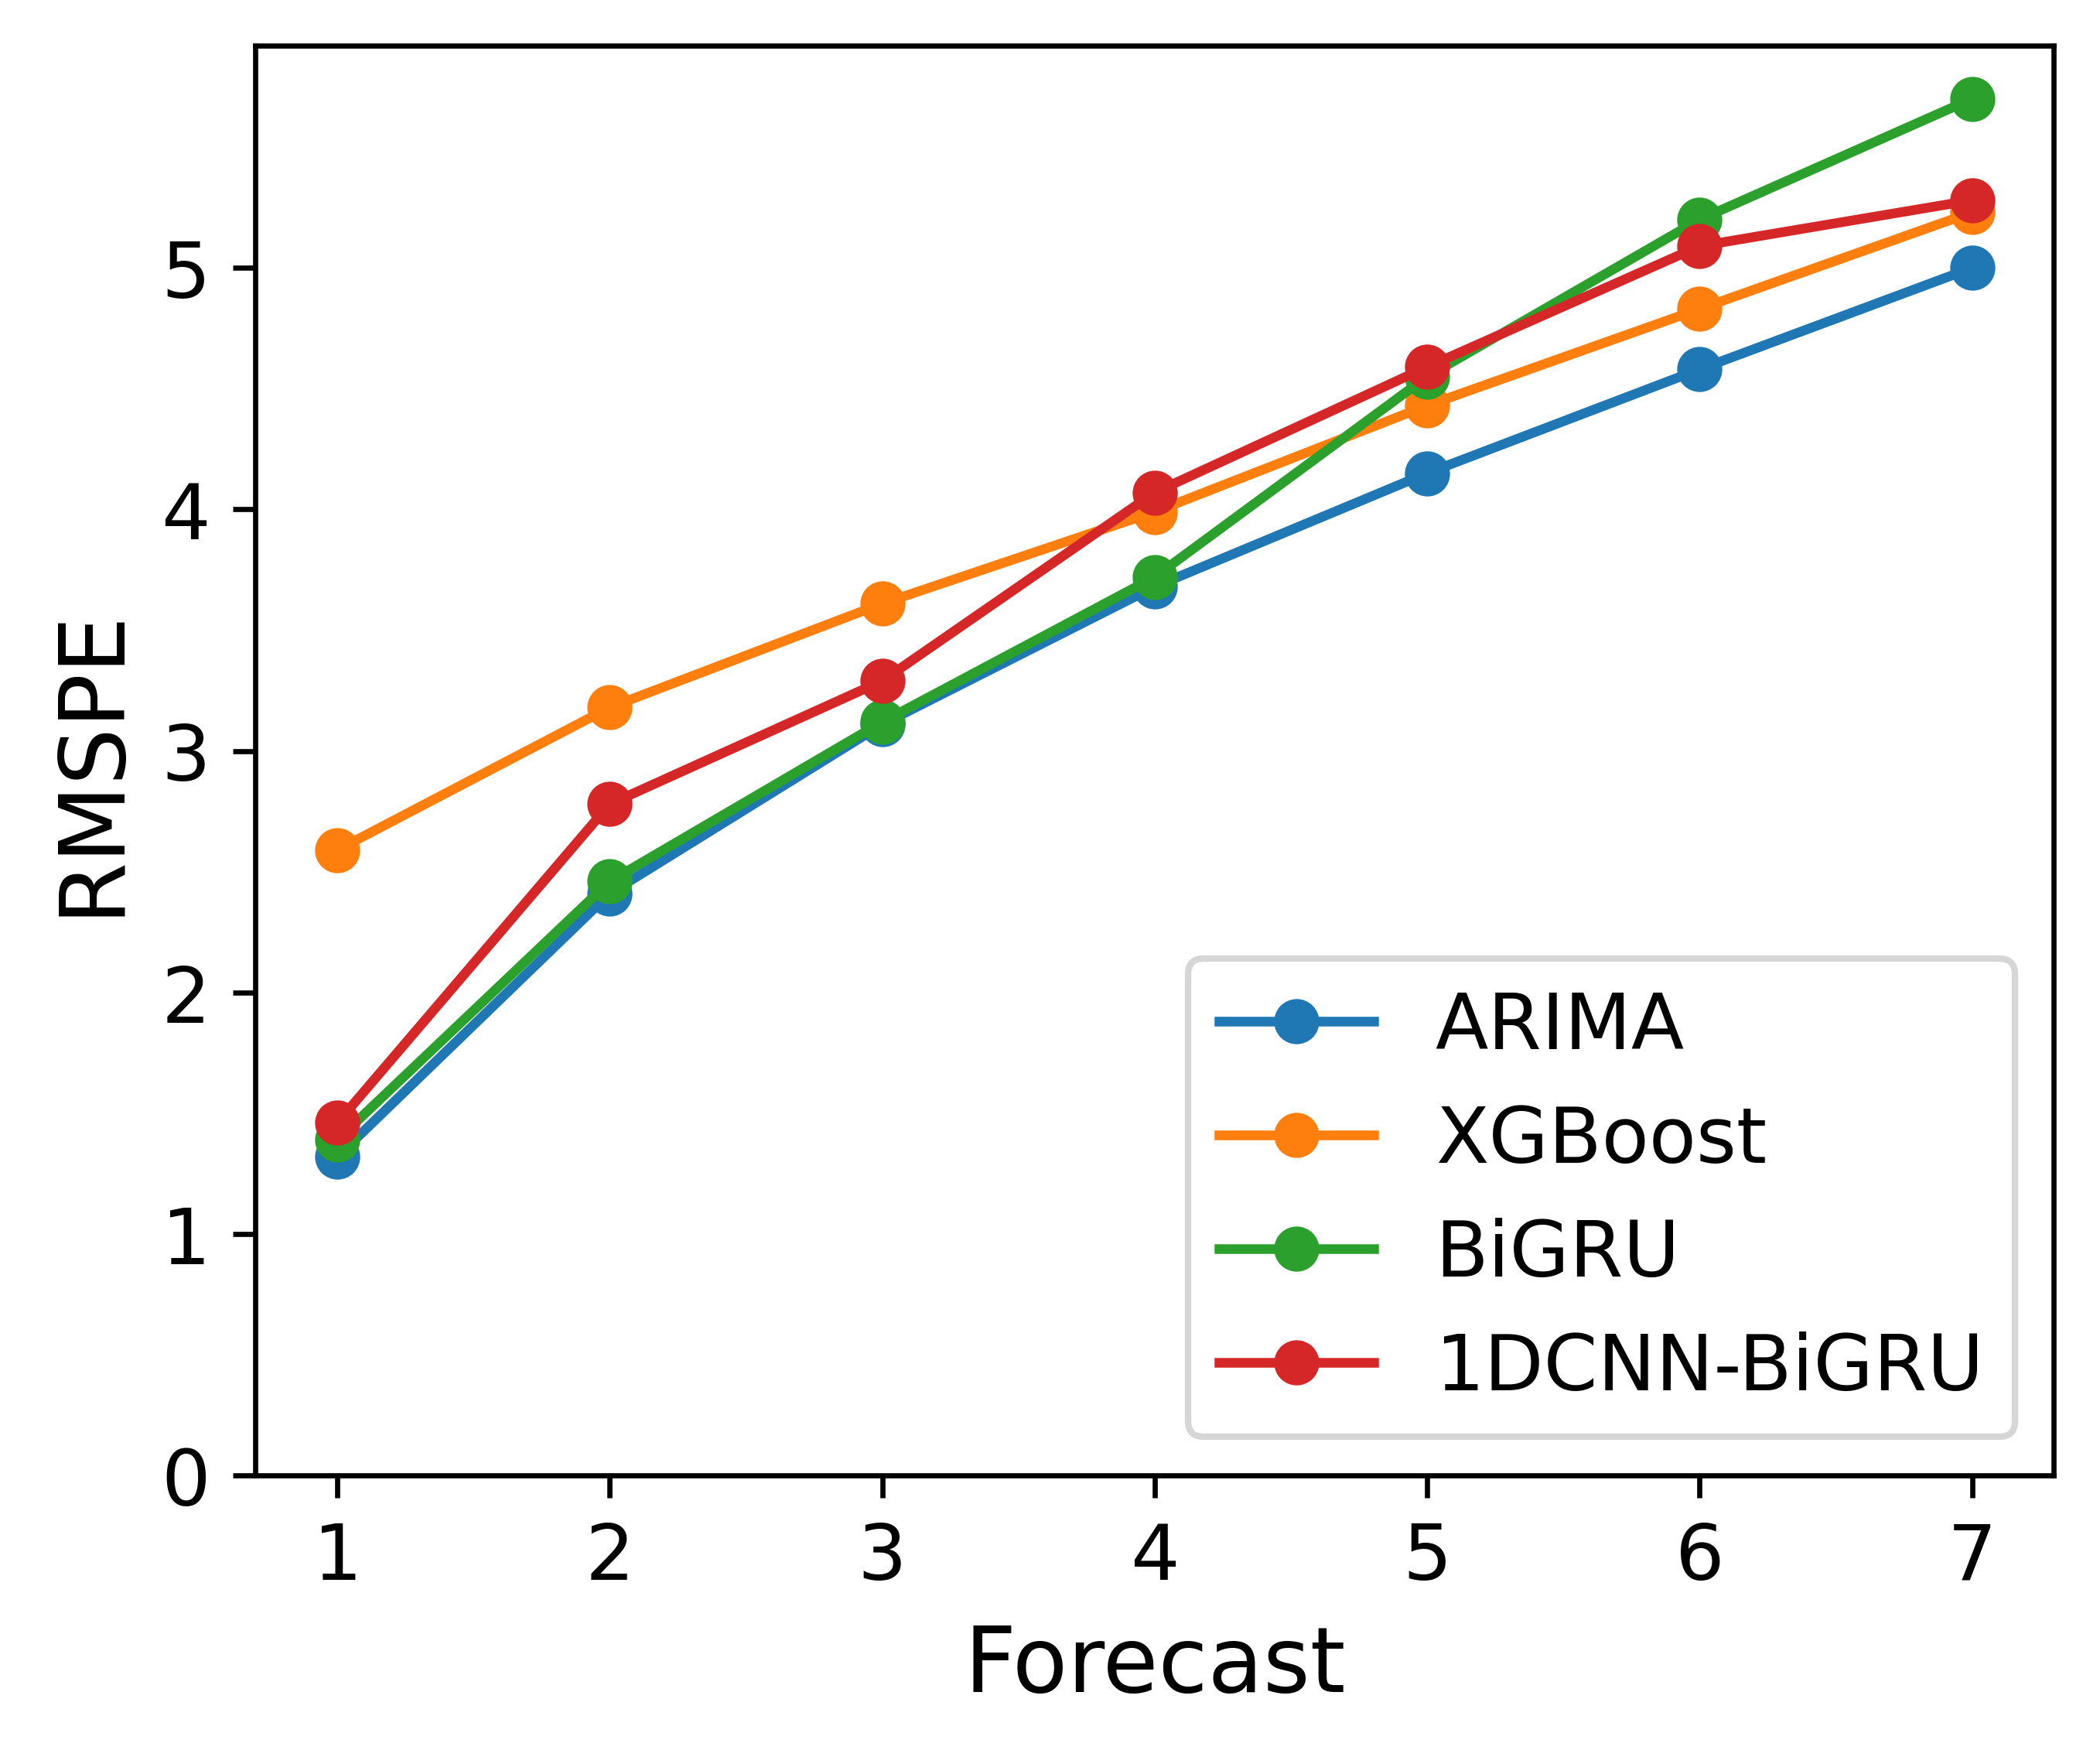
\includegraphics[width=\linewidth]{figures/RMSPE.png}
        \captionof{figure}{Average RMSPE of each model across the 7-day forecast.}
        \label{fig:rmspe}
    \end{figure}
\end{minipage}
\hfill
\begin{minipage}{0.49\textwidth}
    \begin{figure}[H]
        \centering
        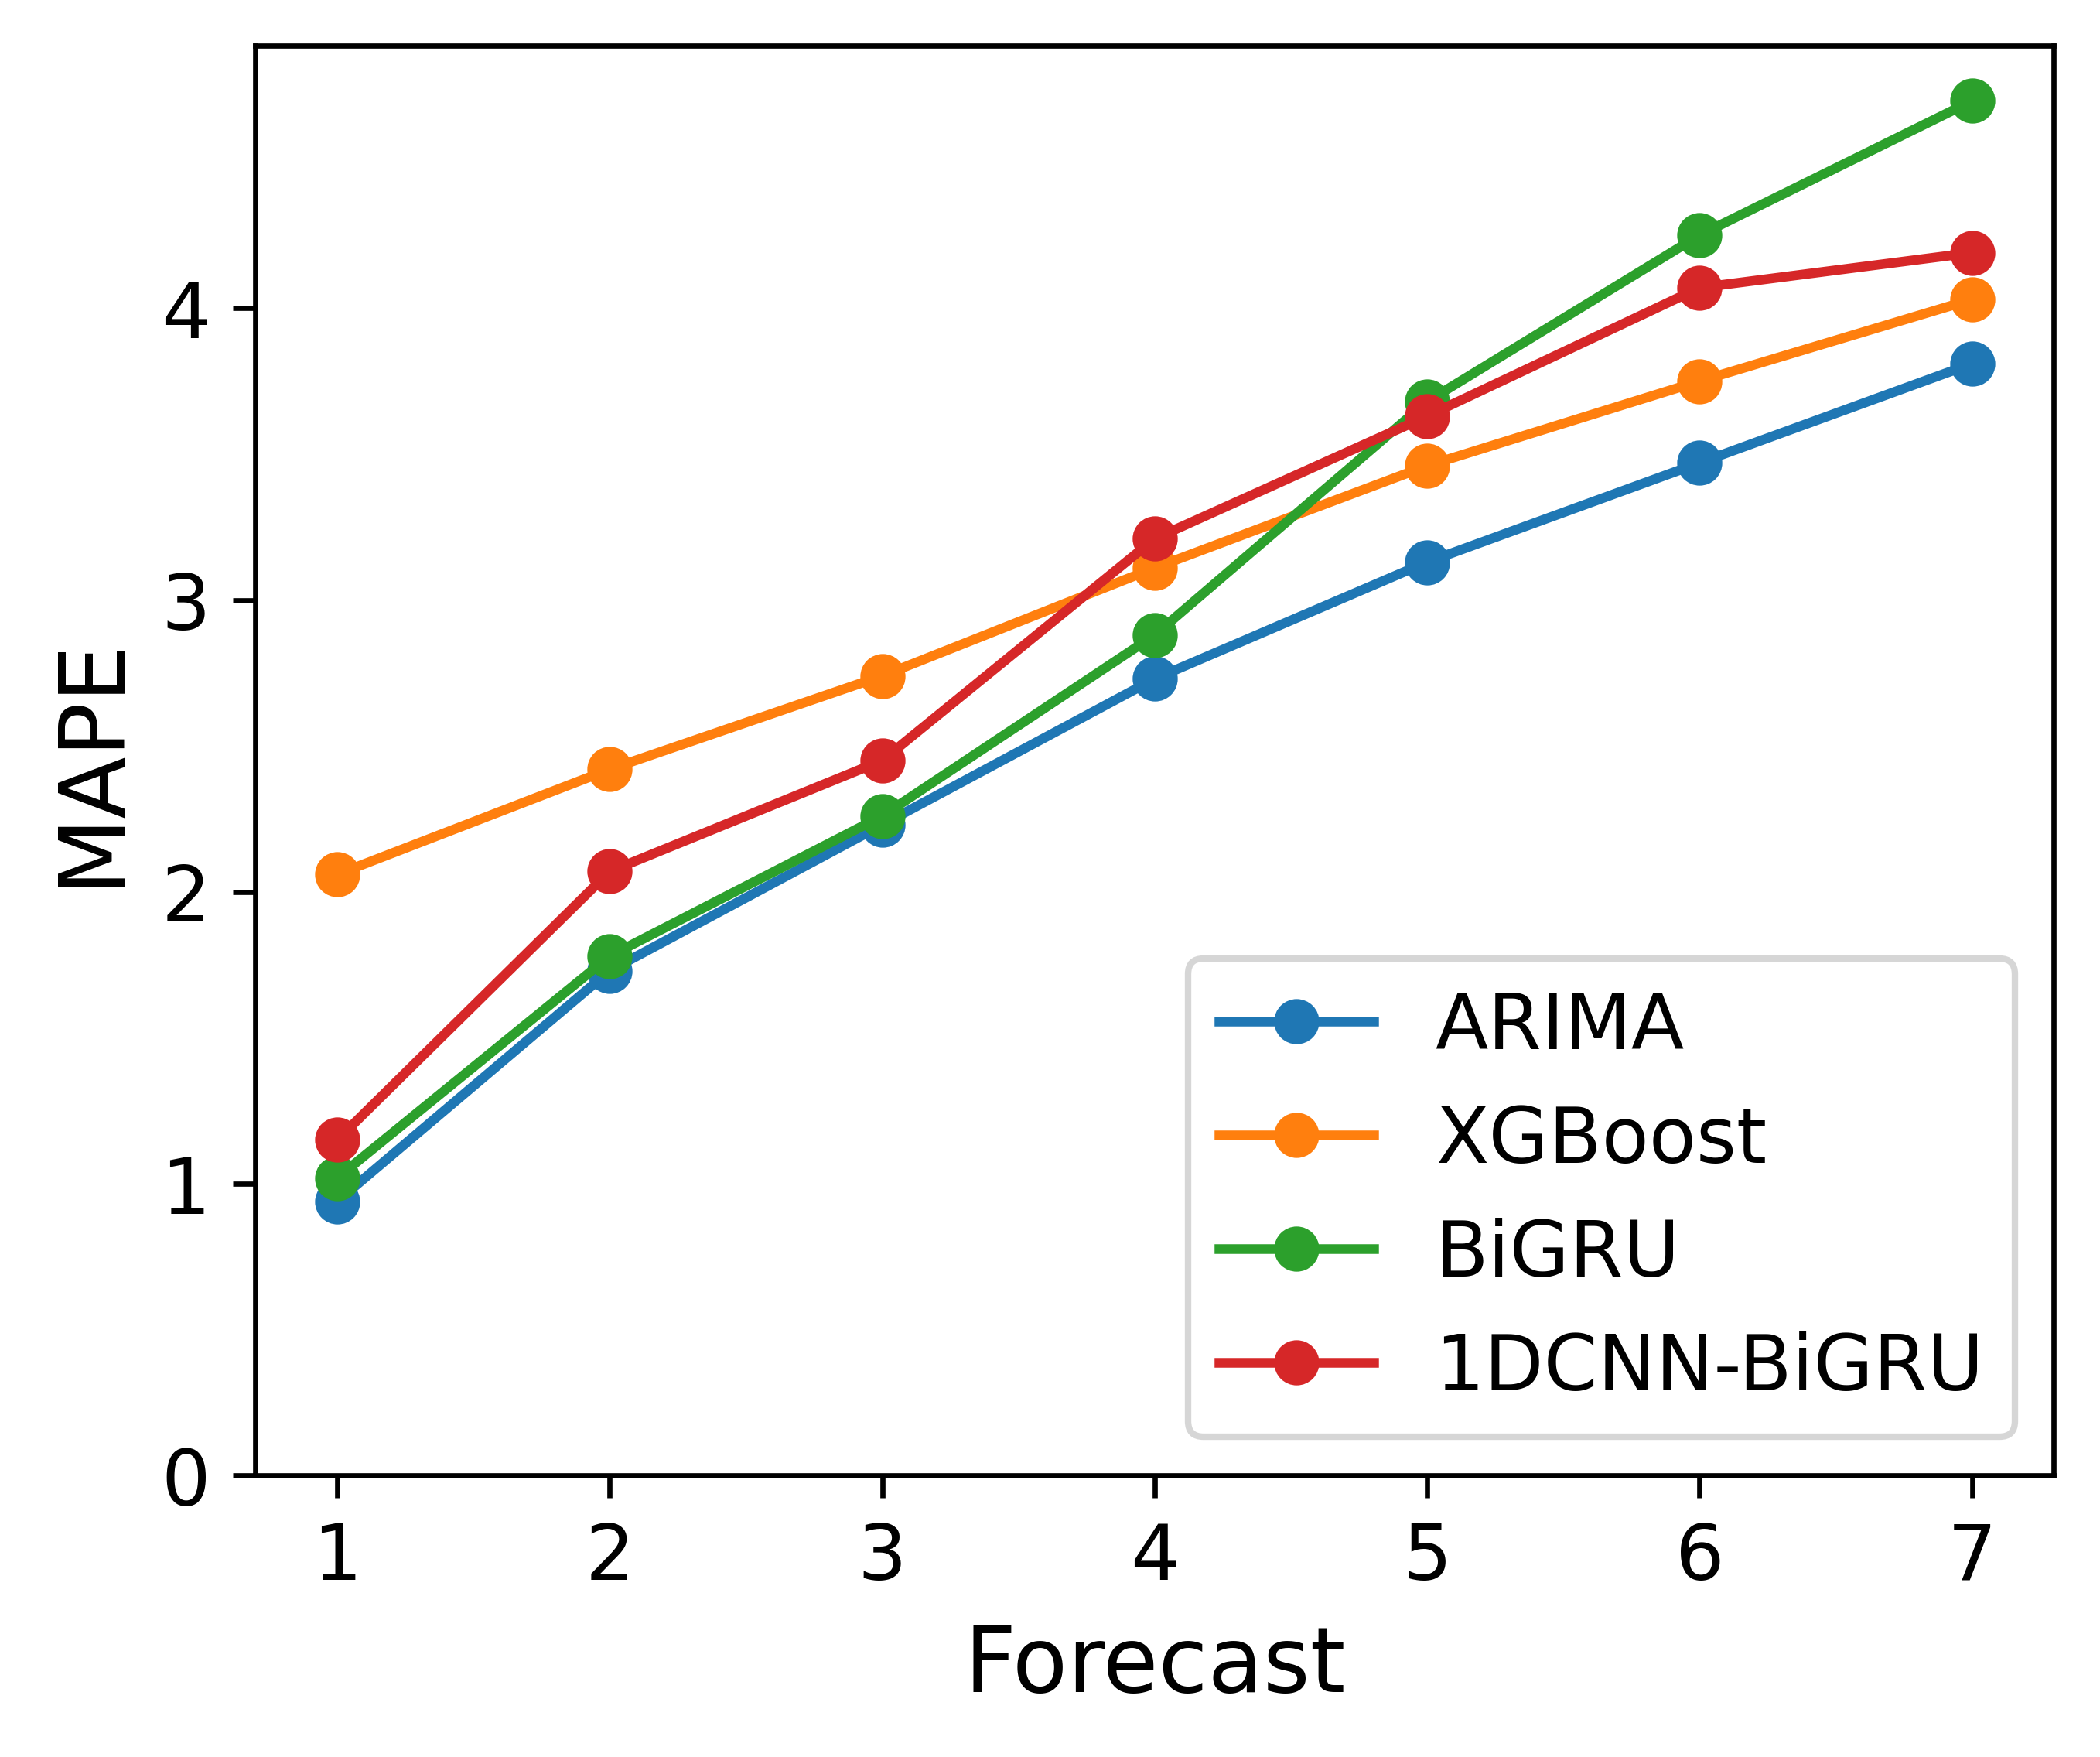
\includegraphics[width=\linewidth]{figures/MAPE.png}
        \captionof{figure}{Average MAPE of each model across the 7-day forecast.}
        \label{fig:mape}
    \end{figure}
\end{minipage}

\captionsetup[figure]{justification=centering}
\noindent
\begin{minipage}{0.49\textwidth}
    \begin{figure}[H]
        \centering
        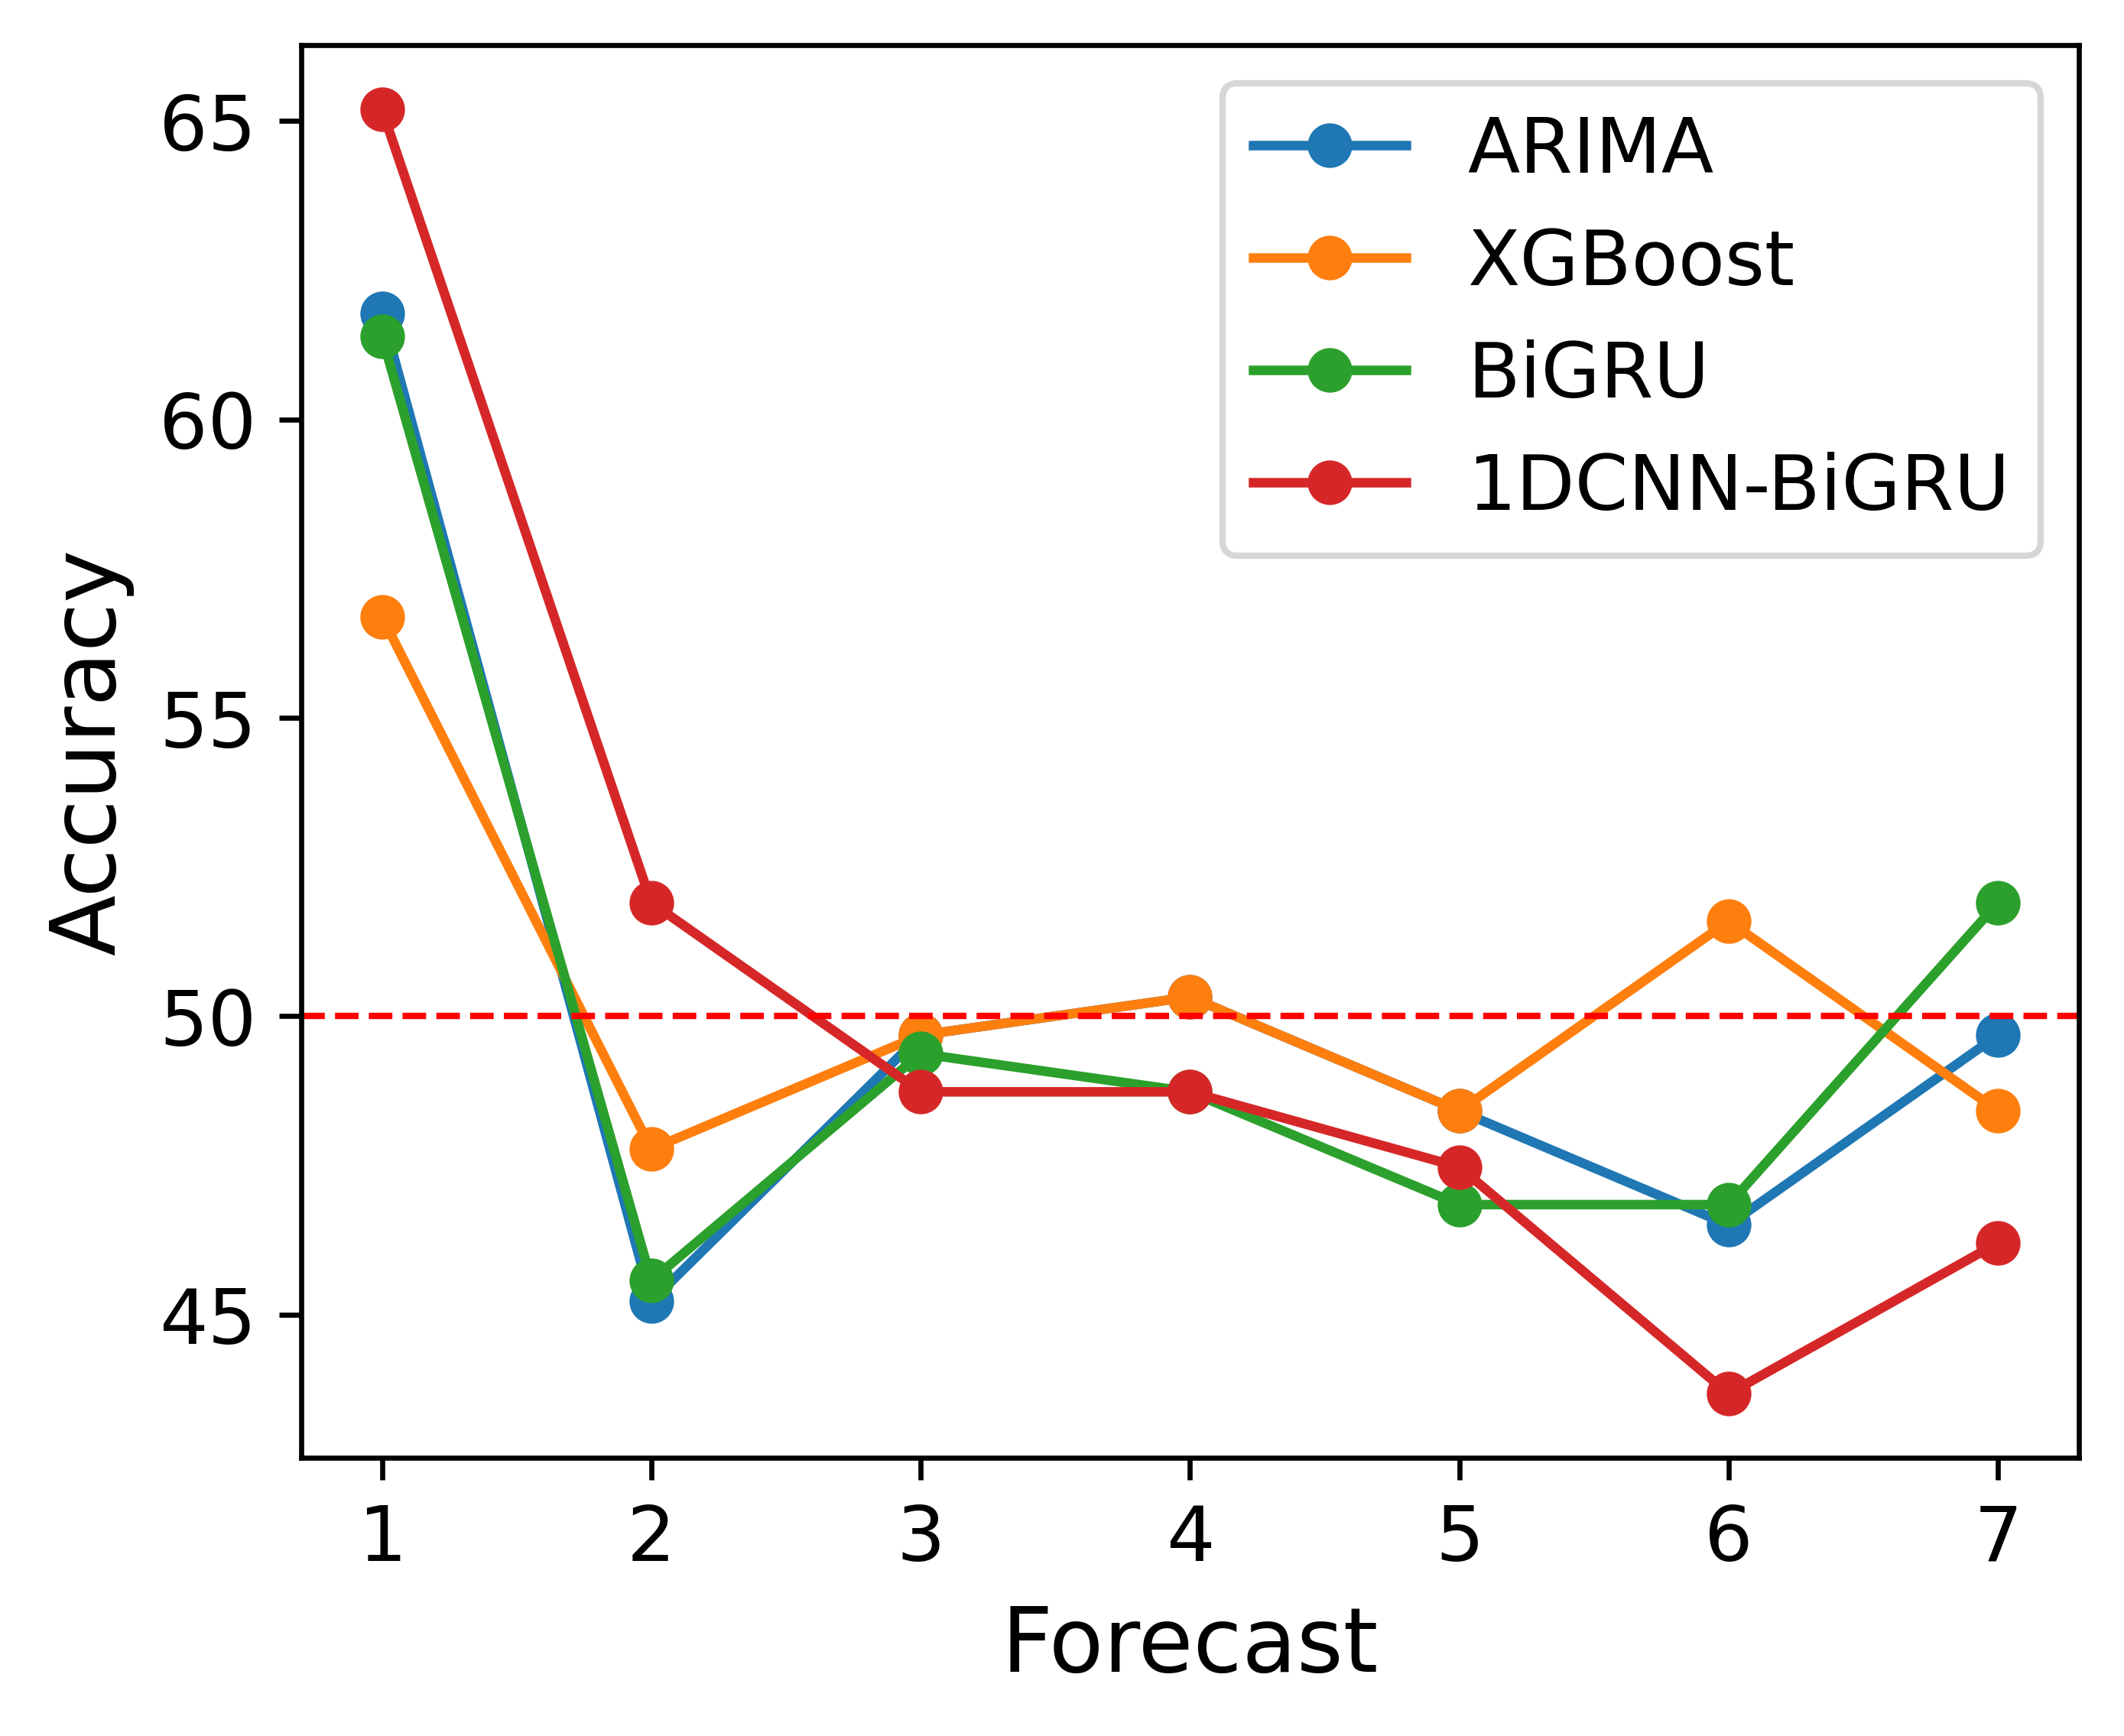
\includegraphics[width=\linewidth]{figures/Accuracy.png}
        \captionof{figure}{Average accuracy of each model across the 7-day forecast.}
        \vspace{0.5cm}
        \label{fig:accuracy}
    \end{figure}
\end{minipage}
\hfill
\begin{minipage}{0.49\textwidth}
    \begin{figure}[H]
        \centering
        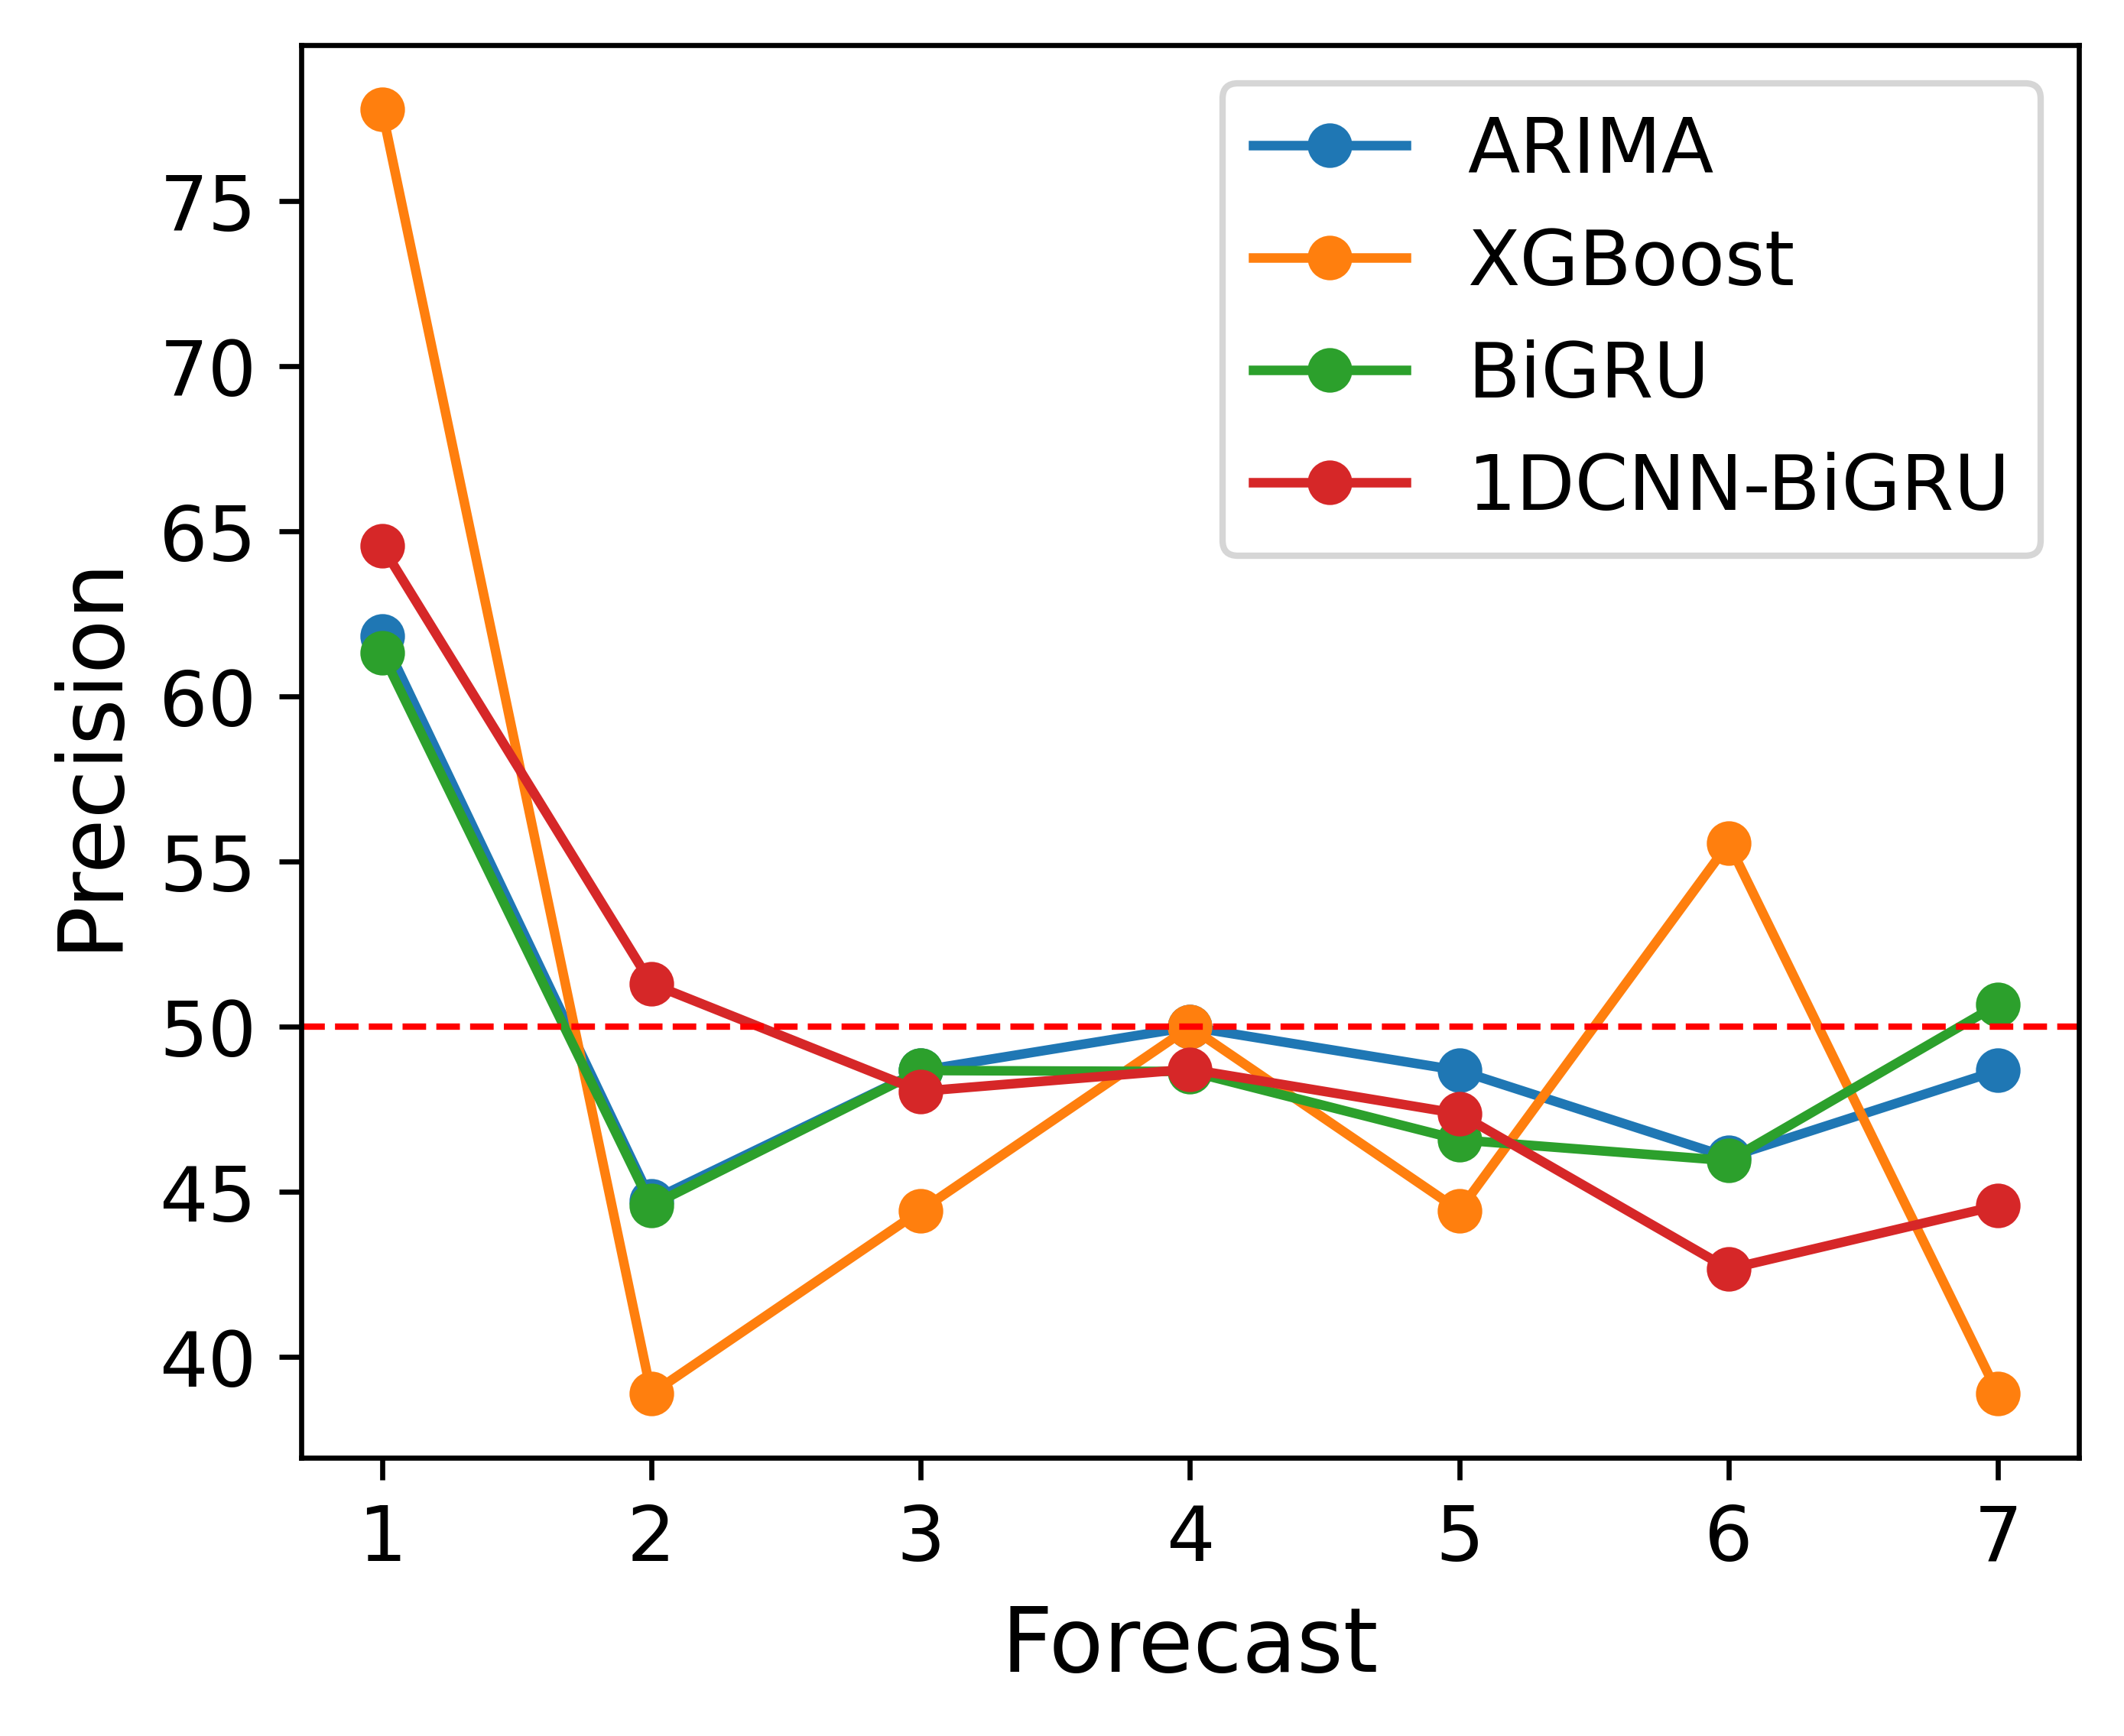
\includegraphics[width=\linewidth]{figures/Precision.png}
        \captionof{figure}{Average precision of each model across the 7-day forecast}
        \vspace{0.5cm}
        \label{fig:precision}
    \end{figure}
\end{minipage}

For a holistic view, Figures \ref{fig:rmspe}-\ref{fig:precision}, show the daily breakdown of each metric for each model. To ensure that the results for the regression metrics are significantly different, Table \ref{tab:wilcoxon} shows the \textit{p}-values of the Wilcoxon signed-rank test, which was carried out on the squared errors of individual forecasts. Using a standard significance level of 0.05, figures in green show that the regression metrics reported are significantly different between the pair of ML models, whereas the figures in red are not.

\begin{table}[h]
\centering
\caption{Wilcoxon signed-rank test \textit{p}-values for pairwise combination of models.}
\label{tab:wilcoxon}
\resizebox{\textwidth}{!}{%
\begin{tabular}{llccccccc}
\toprule
\multirow{2}{*}{\textbf{Model 1}} & \multirow{2}{*}{\textbf{Model 2}} & \multicolumn{7}{c}{\textbf{Forecast}} \\
\cmidrule(lr){3-9}
 & & 1 & 2 & 3 & 4 & 5 & 6 & 7 \\
 \midrule
ARIMA & XGB & \textcolor{green!50!black}{\num{2.38e-14}} & \textcolor{green!50!black}{\num{9.28E-07}} & \textcolor{green!50!black}{\num{1.25E-3}} & \textcolor{green!50!black}{\num{0.0293}} & \textcolor{green!50!black}{\num{0.0368}} & \textcolor{red}{\num{0.110}} & \textcolor{red}{\num{0.217}} \\
ARIMA & BiGRU & \textcolor{green!50!black}{\num{4.13E-3}} & \textcolor{red}{\num{0.487}} & \textcolor{red}{\num{0.924}} & \textcolor{red}{\num{0.216}} & \textcolor{green!50!black}{\num{0.0143}} & \textcolor{green!50!black}{\num{4.37E-3}} & \textcolor{green!50!black}{\num{5.98E-3}} \\
ARIMA & 1DCNN-BiGRU & \textcolor{green!50!black}{\num{7.54E-4}} & \textcolor{green!50!black}{\num{8.88E-4}} & \textcolor{red}{\num{0.0664}} & \textcolor{green!50!black}{\num{7.83E-3}} & \textcolor{green!50!black}{\num{0.0146}} & \textcolor{green!50!black}{\num{0.0165}} & \textcolor{red}{\num{0.609}} \\
XGB   & BiGRU & \textcolor{green!50!black}{\num{1.71E-13}} & \textcolor{green!50!black}{\num{3.26E-6}} & \textcolor{green!50!black}{\num{4.64E-3}} & \textcolor{green!50!black}{\num{0.0297}} & \textcolor{red}{\num{0.670}} & \textcolor{red}{\num{0.147}} & \textcolor{red}{\num{0.0677}} \\
XGB   & 1DCNN-BiGRU & \textcolor{green!50!black}{\num{3.38E-11}} & \textcolor{green!50!black}{\num{9.37E-3}} & \textcolor{green!50!black}{\num{0.0114}} & \textcolor{red}{\num{0.697}} & \textcolor{red}{\num{0.969}} & \textcolor{red}{\num{0.613}} & \textcolor{red}{\num{0.788}} \\
BiGRU & 1DCNN-BiGRU & \textcolor{red}{\num{0.260}} & \textcolor{green!50!black}{\num{2.95E-4}} & \textcolor{red}{\num{0.133}} & \textcolor{green!50!black}{\num{7.45E-4}} & \textcolor{red}{\num{0.455}} & \textcolor{green!50!black}{\num{0.0415}} & \textcolor{green!50!black}{\num{5.22E-3}} \\
\bottomrule
\end{tabular}}
\end{table}

Both Figures \ref{fig:rmspe} and \ref{fig:mape} show a similar pattern, with the only difference being the magnitude of the error. Therefore, considering the results in Table \ref{tab:wilcoxon}, it can be said that ARIMA and BiGRU perform similarly well up until the 4\textsuperscript{th} day of forecast, after which BiGRU's performance starts deteriorating. Although visually it can be seen that the performance of BiGRU and 1DCNN-BiGRU is worse than XGB after the 4\textsuperscript{th}/5\textsuperscript{th} day, based on the significance tests, this claim cannot be firmly made due to the null hypothesis not being rejected. Nevertheless, when the validation and test results are compared, BiGRU is overall the best on a rank basis.

Concerning the classification metrics, the key point in Figures \ref{fig:accuracy} and \ref{fig:precision} is the 1\textsuperscript{st} day of forecast. Although 1DCNN may not always reduce the regression error on BiGRU, it improves the accuracy and precision. Furthermore, XGBoost has significantly higher precision for the 1\textsuperscript{st} day of forecast, suggesting that its strength may be in classification tasks.

To explain the models further, Figure \ref{fig:feature_importances} captures XGBoost, and Figures \ref{fig:bigru_shap} and \ref{fig:1dcnn-bigru_shap} capture both the DNNs. Figure \ref{fig:feature_importances} shows the importance scores by weight for XGBoost, where it shows that it mainly uses the ETH average prices of the previous day to predict the next 7 days. This means that the validation result showing that feature set \Romannum{1} performing the best is a false positive, given that the only ETH blockchain data it is barely making use of is average transaction fees. It is also important to note that the use of just the previous day is something that is common with ARIMA. As a result of calculating feature importances, two limitations of XGBoost were also highlighted. First, feature importance by total gain can not be calculated with a multi-output strategy, as the Python library does not currently allow for it. Second, a multi-output strategy is something that the Shapley Additive Explanations (SHAP) method also does not support; therefore, SHAP values could not be generated in the same manner as done for BiGRU and 1DCNN-BiGRU. Figures \ref{fig:bigru_shap} and \ref{fig:1dcnn-bigru_shap} show the average SHAP values for BiGRU and 1DCNN-BiGRU across the 7-day forecast horizon and the 14-day lags, respectively. Both show an oscillating pattern, where every other day has positive values, suggesting an improved effect in the forecast. The only difference between the two is that BiGRU's oscillation ends around day 10, and 1DCNN-BiGRU's oscillation ends around day 7, which is in line with \textit{k} value of 7. This difference between the two is what makes BiGRU more performative in the test set than 1DCNN-BiGRU. It is also interesting to note that even though both models take 14 days of lag, only a fraction of that has a positive impact on the prediction.
% \begin{table}[h]
% \centering
% \caption{Bonferroni corrected p-values for Wilcoxon signed-rank test for pairwise combination of models.}
% \resizebox{\textwidth}{!}{%
% \begin{tabular}{llccccccc}
% \toprule
% \multirow{2}{*}{\textbf{Model 1}} & \multirow{2}{*}{\textbf{Model 2}} & \multicolumn{7}{c}{\textbf{Forecast}} \\
% \cmidrule(lr){3-9}
%  & & 1 & 2 & 3 & 4 & 5 & 6 & 7 \\
%  \midrule
% ARIMA & XGB & \textcolor{green!50!black}{\num{1.43e-13}} & \textcolor{green!50!black}{\num{5.57E-06}} & \textcolor{green!50!black}{\num{7.50E-03}} & \textcolor{red}{\num{0.176}} & \textcolor{red}{\num{0.221}} & \textcolor{red}{\num{0.661}} & \textcolor{red}{\num{1.30}} \\
% ARIMA & BiGRU & \textcolor{green!50!black}{\num{0.0248}} & \textcolor{red}{\num{2.92}} & \textcolor{red}{\num{5.54}} & \textcolor{red}{\num{1.30}} & \textcolor{red}{\num{0.0859}} & \textcolor{green!50!black}{\num{0.0262}} & \textcolor{green!50!black}{\num{0.0359}} \\
% ARIMA & 1DCNN-BiGRU & \textcolor{green!50!black}{\num{4.55E-3}} & \textcolor{green!50!black}{\num{5.33E-3}} & \textcolor{red}{\num{0.398}} & \textcolor{green!50!black}{\num{0.0470}} & \textcolor{red}{\num{0.0876}} & \textcolor{red}{\num{0.0988}} & \textcolor{red}{\num{0.609}} \\
% XGB   & BiGRU & \textcolor{green!50!black}{\num{1.03E-12}} & \textcolor{green!50!black}{\num{1.95E-05}} & \textcolor{green!50!black}{\num{0.0278}} & \textcolor{red}{\num{0.178}} & \textcolor{red}{\num{4.02}} & \textcolor{red}{\num{0.879}} & \textcolor{red}{\num{0.406}} \\
% XGB   & 1DCNN-BiGRU & \textcolor{green!50!black}{\num{2.03E-10}} & \textcolor{red}{\num{0.0562}} & \textcolor{red}{\num{0.0681}} & \textcolor{red}{\num{4.18}} & \textcolor{red}{\num{5.81}} & \textcolor{red}{\num{3.68}} & \textcolor{red}{\num{4.73}} \\
% BiGRU & 1DCNN-BiGRU & \textcolor{red}{\num{1.56}} & \textcolor{green!50!black}{\num{1.77E-3}} & \textcolor{red}{\num{0.796}} & \textcolor{green!50!black}{\num{4.47E-3}} & \textcolor{red}{\num{2.73}} & \textcolor{red}{\num{0.249}} & \textcolor{green!50!black}{\num{0.0313}} \\
% \bottomrule
% \end{tabular}}
% \end{table}

\begin{figure}[H]
    \centering
    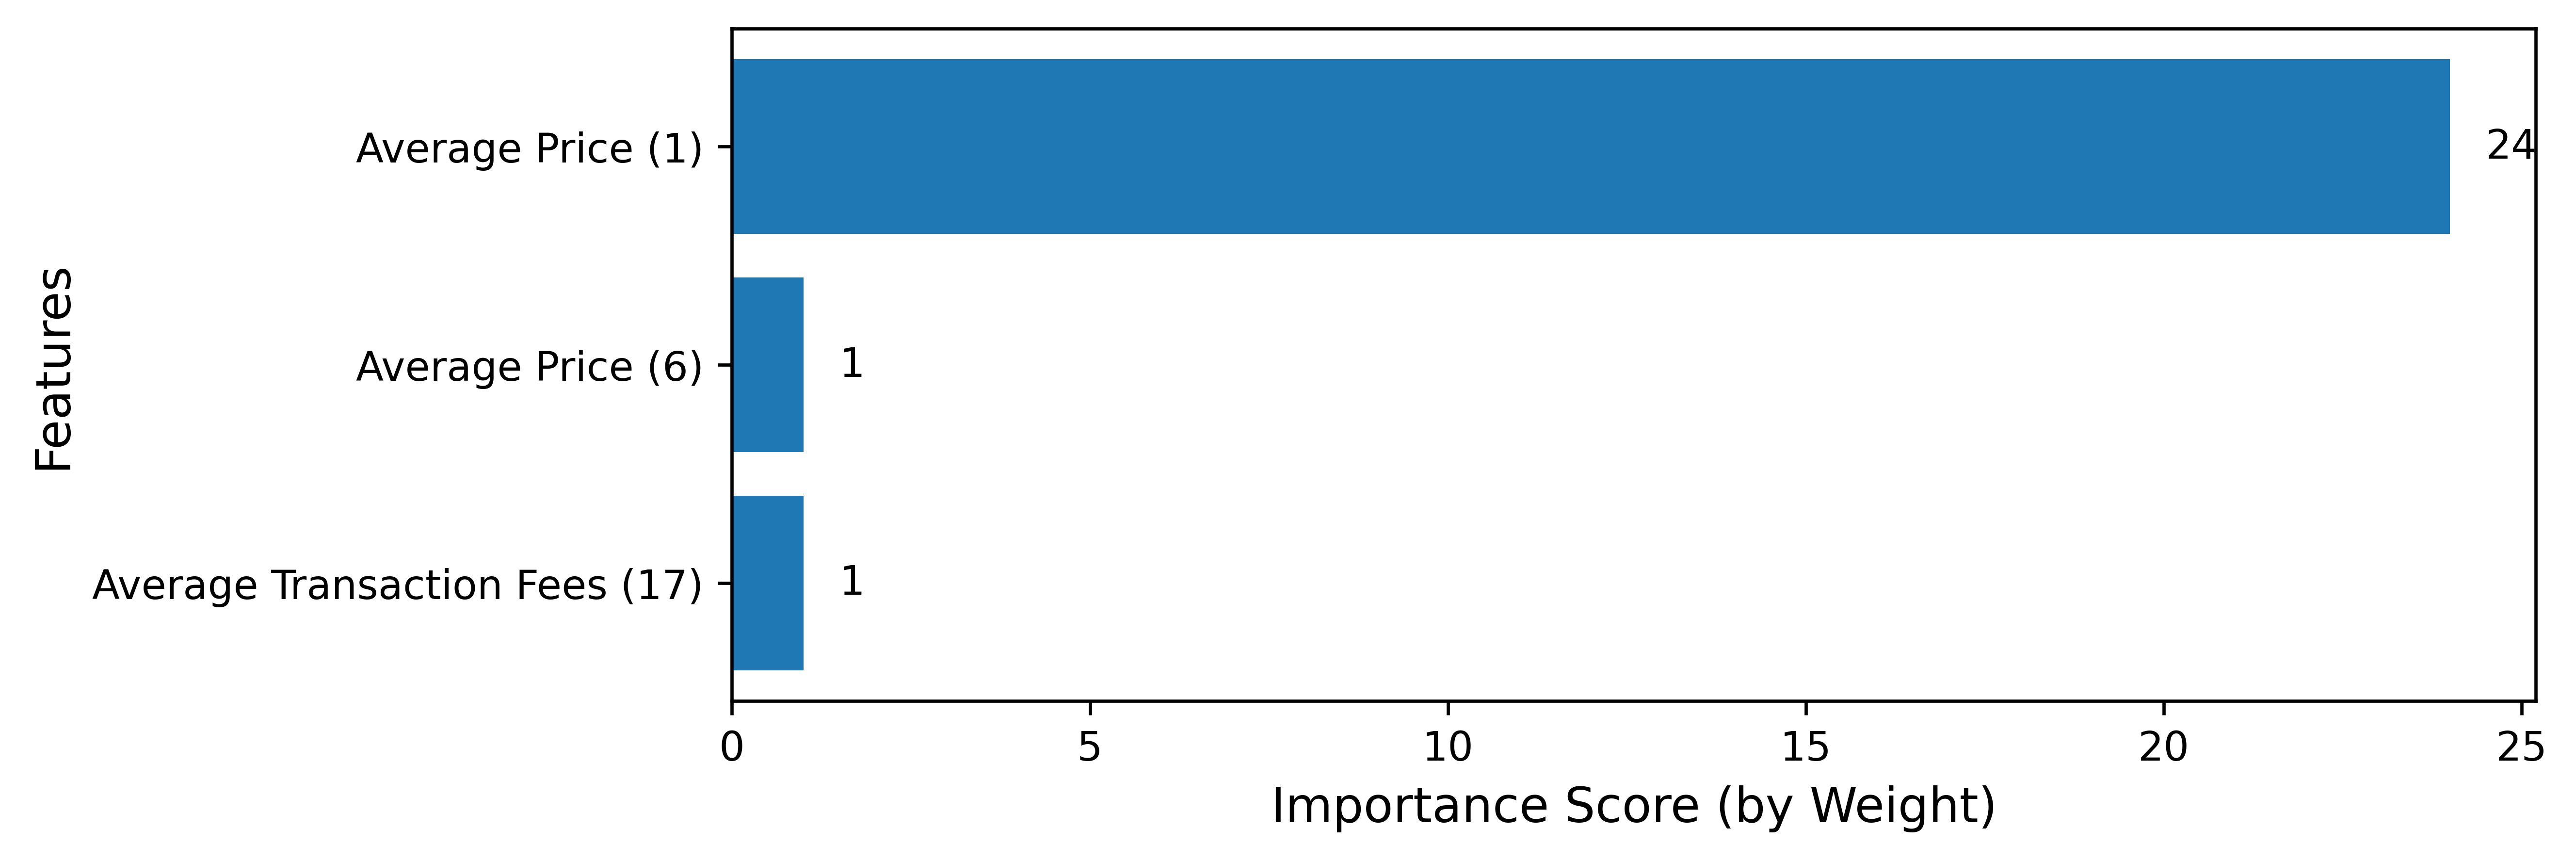
\includegraphics[width=1\linewidth]{figures/feature_importances.png}
    \caption{XGBoost feature importances by weight.}
    \label{fig:feature_importances}
\end{figure}

\captionsetup[figure]{justification=centering}
\noindent
\begin{minipage}{0.49\textwidth}
    \begin{figure}[H]
        \centering
        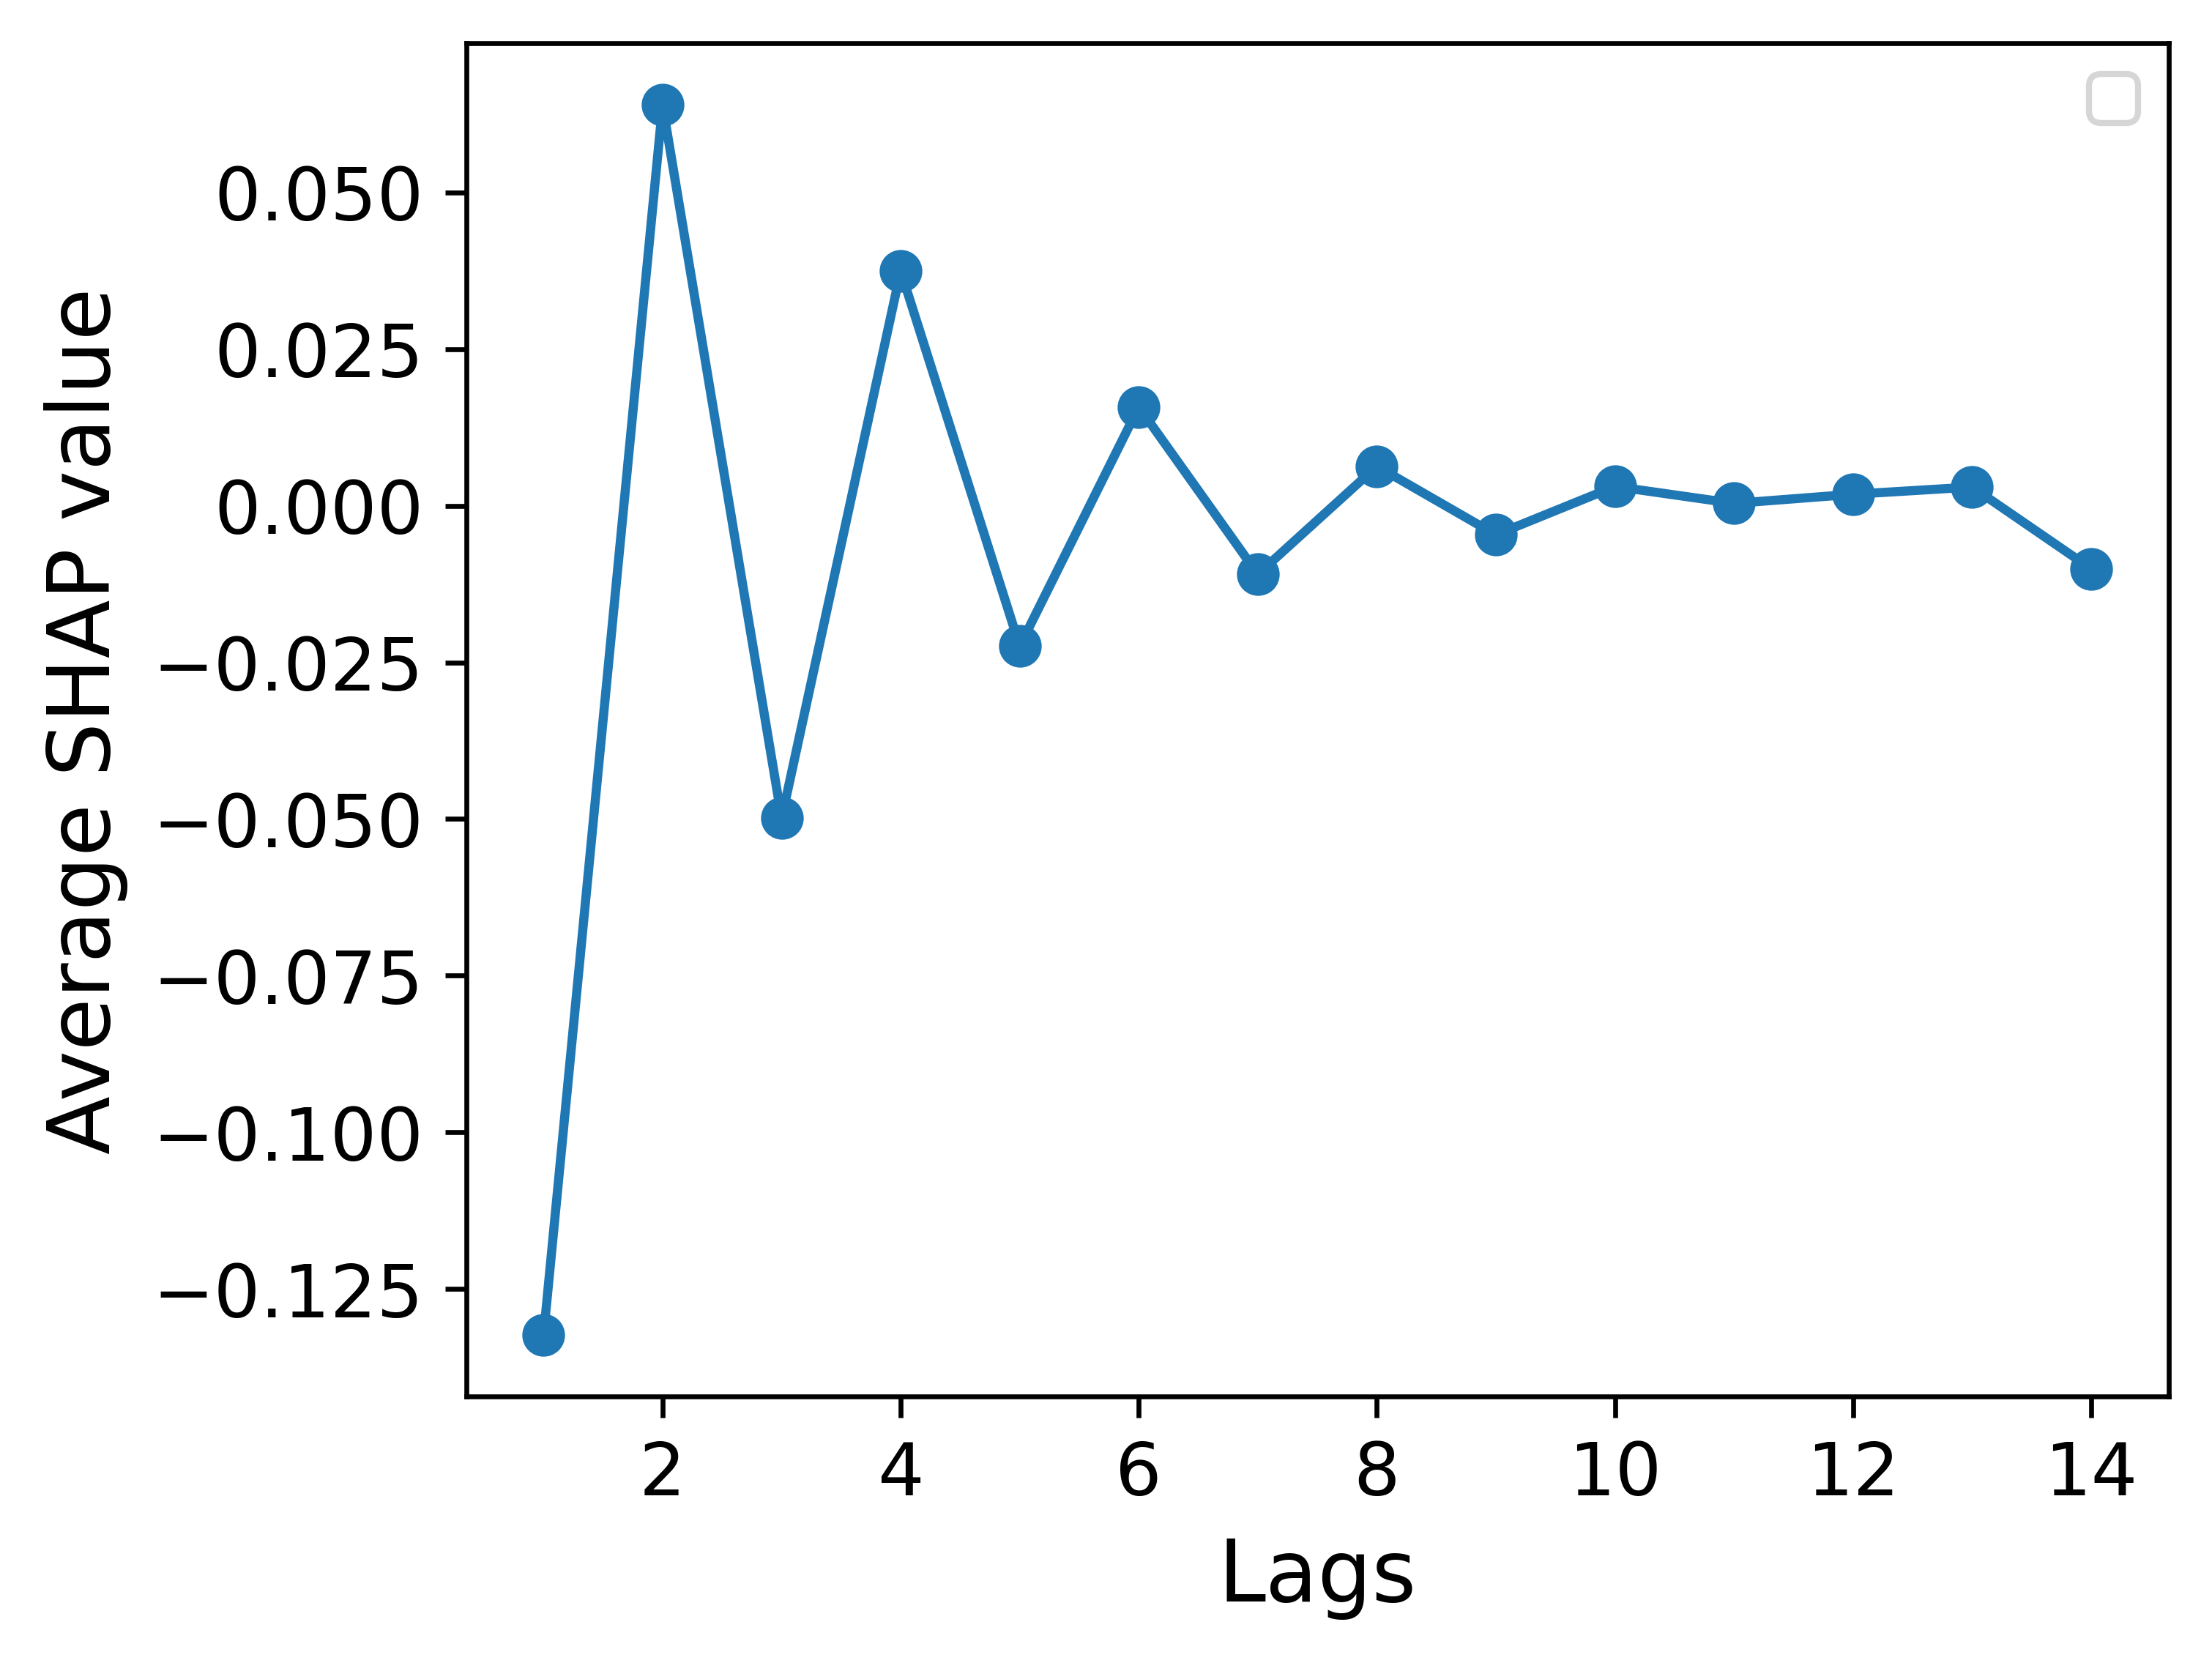
\includegraphics[width=\linewidth]{figures/bigru_shap.png}
        \captionof{figure}{Average SHAP values of the BiGRU model evaluated across all lags.}
        \vspace{0.7cm}
        \label{fig:bigru_shap}
    \end{figure}
\end{minipage}
\hfill
\begin{minipage}{0.49\textwidth}
    \begin{figure}[H]
        \centering
        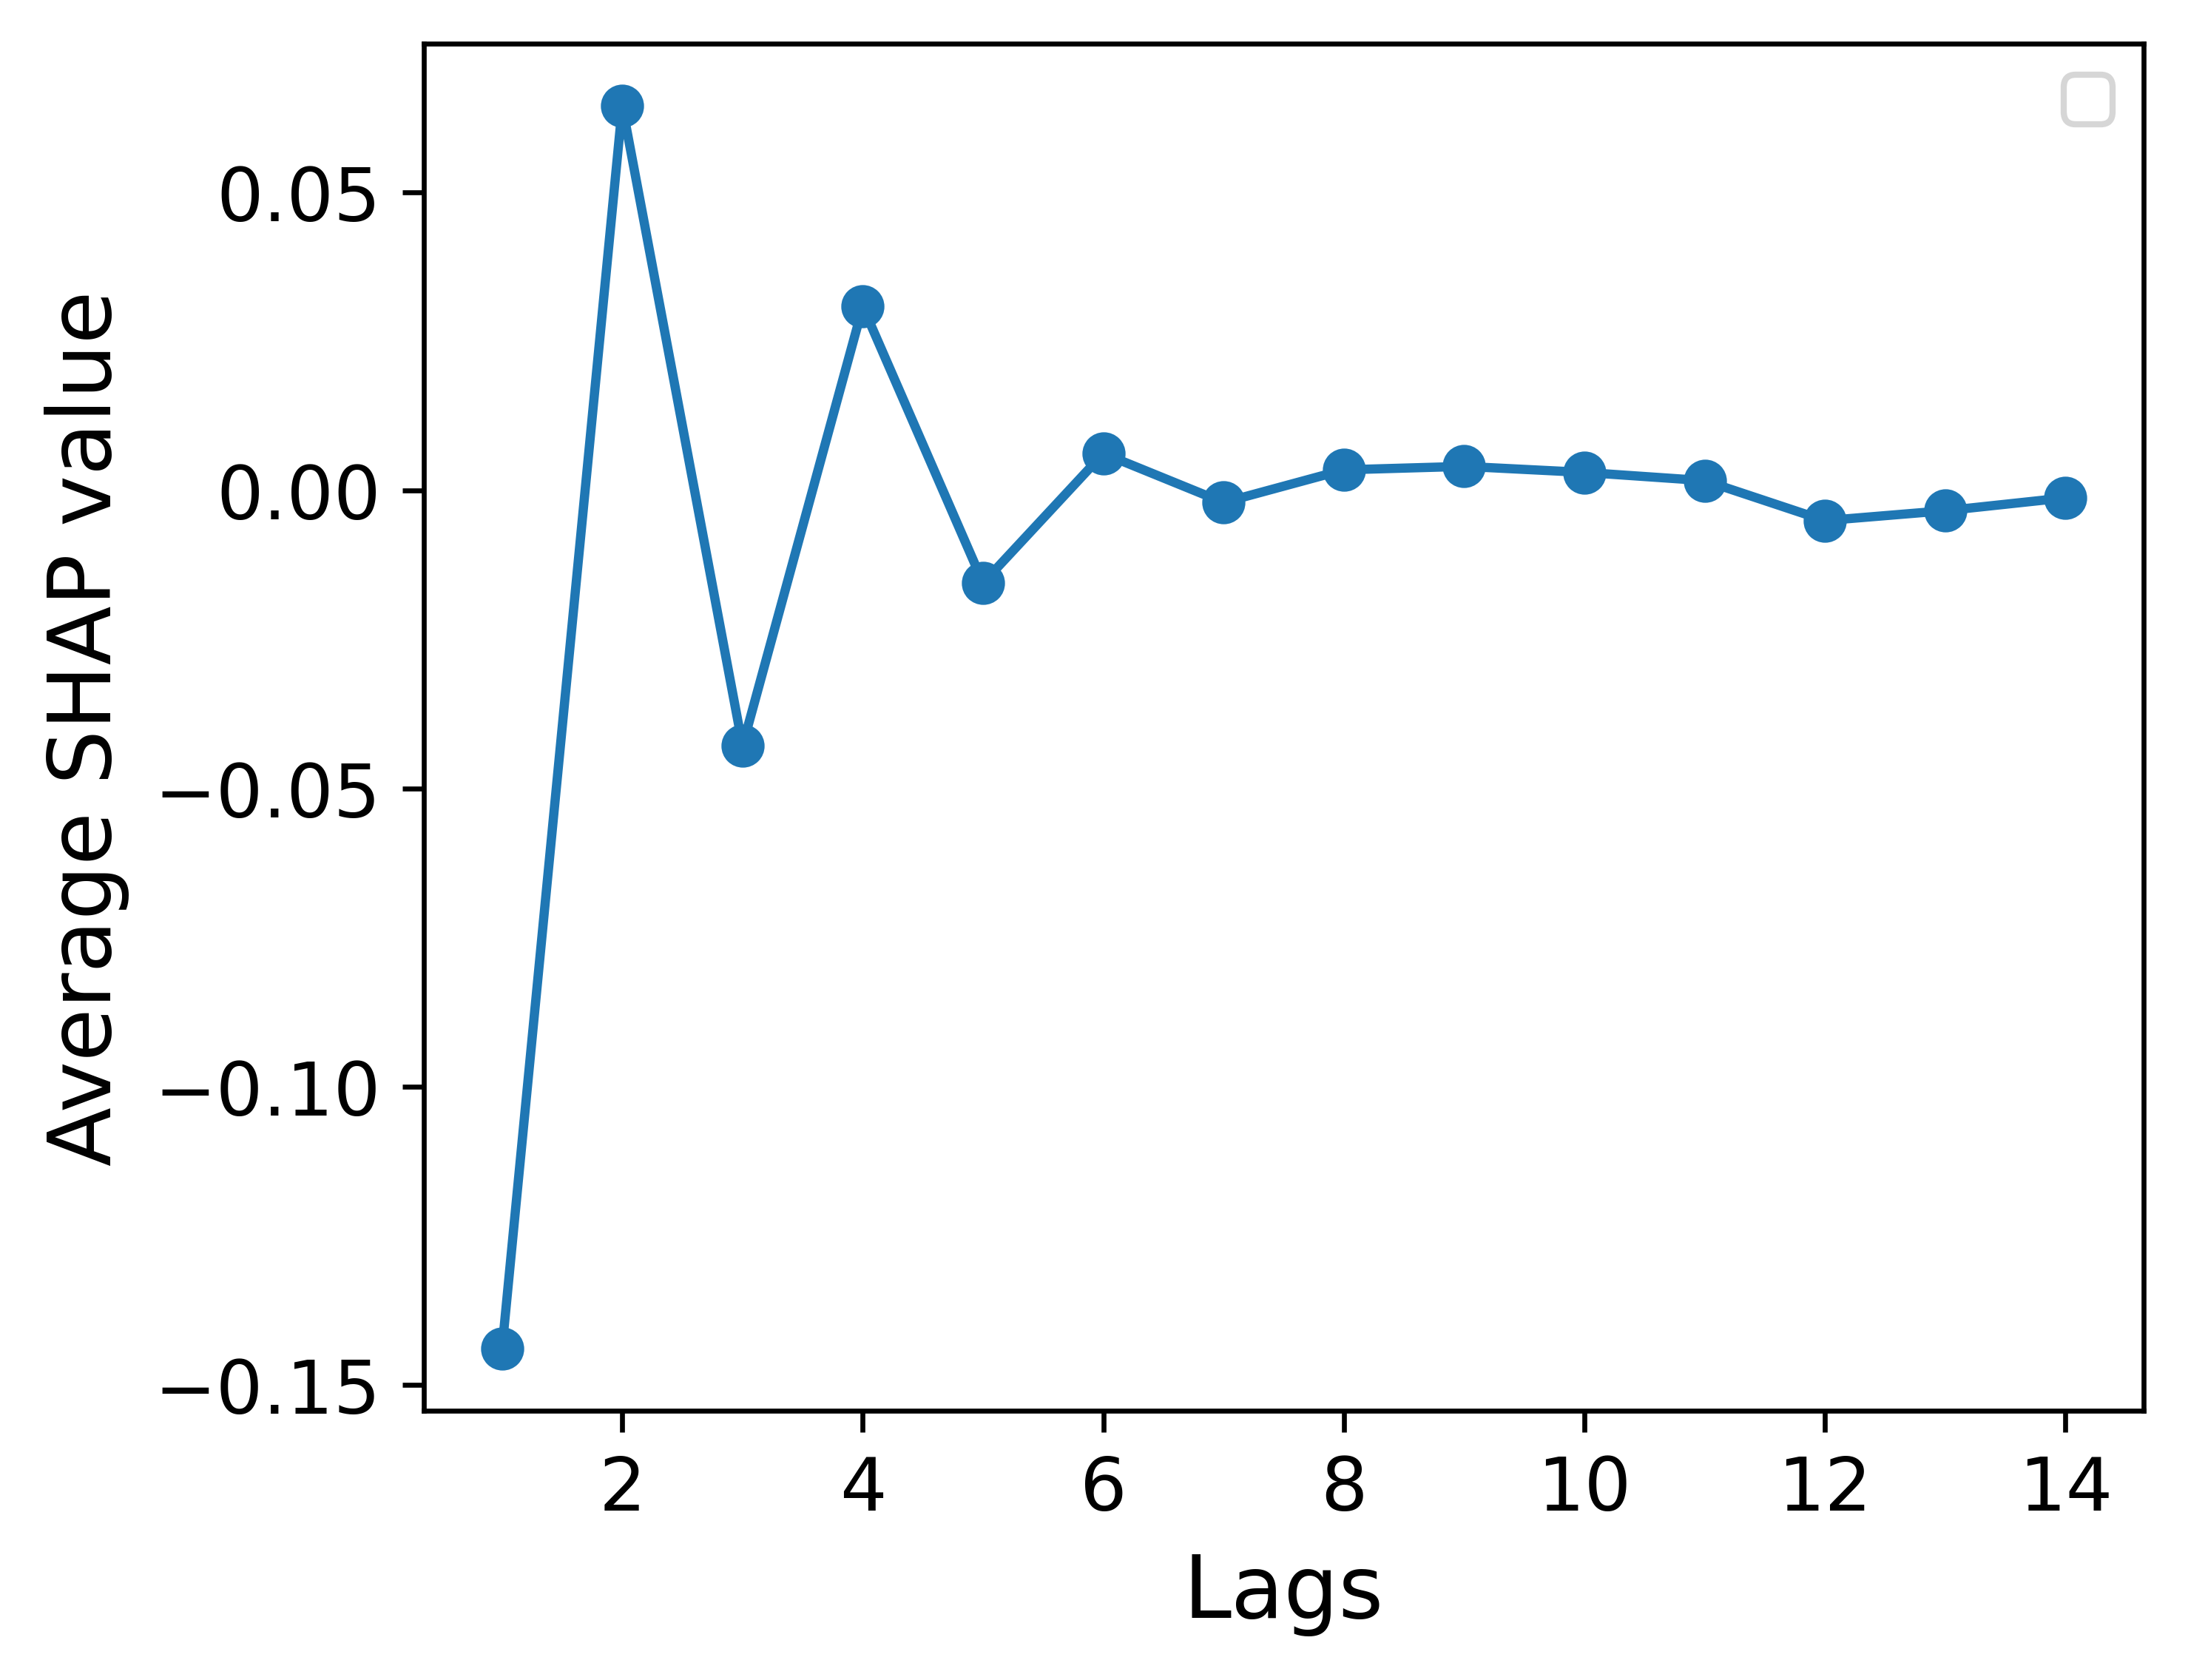
\includegraphics[width=\linewidth]{figures/1dcnn-bigru_shap.png}
        \captionof{figure}{Average SHAP values of the 1DCNN-BiGRU model evaluated across all lags.}
        \vspace{0.7cm}
        \label{fig:1dcnn-bigru_shap}
    \end{figure}
\end{minipage}

% {\bf A topic-specific chapter, roughly 30\% of the total page-count} 
% \vspace{1cm} 

% \noindent
% This chapter is intended to evaluate what you did.  The content is highly 
% topic-specific, but for many projects will have flavours of the following:

% \begin{enumerate}
% \item functional  testing, including analysis and explanation of failure 
%       cases,
% \item behavioural testing, often including analysis of any results that 
%       draw some form of conclusion wrt. the aims and objectives,
%       and
% \item evaluation of options and decisions within the project, and/or a
%       comparison with alternatives.
% \end{enumerate}

% \noindent
% This chapter often acts to differentiate project quality: even if the work
% completed is of a high technical quality, critical yet objective evaluation 
% and comparison of the outcomes is crucial.  In essence, the reader wants to
% learn something, so the worst examples amount to simple statements of fact 
% (e.g., ``graph X shows the result is Y''); the best examples are analytical 
% and exploratory (e.g., ``graph X shows the result is Y, which means Z; this 
% contradicts [1], which may be because I use a different assumption'').  As 
% such, both positive {\em and}\/ negative outcomes are valid {\em if} presented 
% in a suitable manner.

% -----------------------------------------------------------------------------

\chapter{Conclusion}
\label{chap:conclusion}
The aim of this research was to investigate whether blockchain data (internal factors) and/or sentiment analysis of news headlines (external factors) can improve the predictive performance of ML models. This was achieved by building on the work done by Kim \textit{et al.} \cite{RN141} and successfully completing all objectives of this project, so that the validity of their results can be reevaluated for Ethereum 2.0. This chapter serves as a concluding remark to emphasise the project's contributions to the research community, summarise the key findings in relation to Kim's work, and outline potential directions for future research.

\section{Key Contributions}
The key contribution of this thesis is twofold: methodological improvement of Kim's work, followed by a novel extension that includes the experimentation of various sentiment analysis methods on news headlines. The first part of the methodological improvement looked at having a good feature selection step, setting a baseline feature set and a baseline model, all of which were crucial in judging the effectiveness of the features. The second part focused on improving the real-world applicability of this research for traders by having a forecast horizon of 7 days, but also by using percentage-based metrics to assess error margin in the prices as well as directional accuracy. The last part looked at increasing confidence in the results, and this was done through significance testing and explainable AI methods. 

\section{Key Findings}
The initial hypotheses from Kim's study were disproven by the findings of this project. Neither the blockchain data of ETH nor that of the highly correlated cryptocurrencies improves the predictive performance of ML models. Though sentiment analysis of news headlines did not show improvement on top of the baseline feature set, it is believed that this was due to a lack of properly capturing the magnitude of influence of each news. Therefore, making any firm conclusions without further testing would not be wise. Nevertheless, BiGRU was still proven to be the best model across both validation and test sets. It was also interesting to see that a simpler statistical model like ARIMA could also perform equally well. Furthermore, both XGBoost and ARIMA demonstrated that the prediction of the next 7 days was heavily influenced by the previous day of lag. 

\section{Future Work}
One of the limitations of the work in this project is the use of an exhaustive hyperparameter tuning strategy. The implication of this mainly is on DNNs, given that they not only require careful hyperparameter tuning but are also computationally expensive, which limits the search space size when using grid search. This is one area of improvement, where more intelligent methods, such as Bayesian search, would be useful to consolidate the results. Another limitation was that the acquired news headlines did not have any data regarding public engagement or the magnitude of influence. Testing with the inclusion of such data would give new information to conclude on the effectiveness of news headlines. A key challenge to implementing this for future work would be acquiring such data. Lastly, future work could consider the use of other types of models. Currently, transformers are under-researched \cite{john2024cryptocurrency}, and are a good candidate to see if it can better generalise patterns in comparison to typical RNNs. 

% {\bf A compulsory chapter,  roughly 10\% of the total page-count}
% \vspace{1cm} 

% \noindent
% The concluding chapter(s) of a dissertation are often underutilized because they're 
% too often left too close to the deadline: it is important to allocate enough time and 
% attention to closing off the story, the narrative, of your thesis.

% Again, there is no single correct way of closing a thesis. 

% One good way of doing this is to have a single chapter consisting of three parts:

% \begin{enumerate}
% \item (Re)summarise the main contributions and achievements, in essence
%       summing up the content.
% \item Clearly state the current project status (e.g., ``X is working, Y 
%       is not'') and evaluate what has been achieved with respect to the 
%       initial aims and objectives (e.g., ``I completed aim X outlined 
%       previously, the evidence for this is within Chapter Y'').  There 
%       is no problem including aims which were not completed, but it is 
%       important to evaluate and/or justify why this is the case.
% \item Outline any open problems or future plans.  Rather than treat this
%       only as an exercise in what you {\em could} have done given more 
%       time, try to focus on any unexplored options or interesting outcomes
%       (e.g., ``my experiment for X gave counter-intuitive results, this 
%       could be because Y and would form an interesting area for further 
%       study'' or ``users found feature Z of my software difficult to use,
%       which is obvious in hindsight but not during at design stage; to 
%       resolve this, I could clearly apply the technique of Bloggs {\em et al.}.
% \end{enumerate}

% Alternatively, you might want to divide this content into two chapters: a penultimate chapter with a title such as ``Further Work" and then a final chapter ``Conclusions". Again, there is no hard and fast rule, we trust you to make the right decision. 

% And this, the final paragraph of this thesis template, is just a bunch of citations, added to show how to generate a BibTeX bibliography. Sources that have been randomly chosen to be cited here include.




% =============================================================================

% Finally, after the main matter, the back matter is specified.  This is
% typically populated with just the bibliography.  LaTeX deals with these
% in one of two ways, namely
%
% - inline, which roughly means the author specifies entries using the 
%   \bibitem macro and typesets them manually, or
% - using BiBTeX, which means entries are contained in a separate file
%   (which is essentially a database) then imported; this is the 
%   approach used below, with the databased being dissertation.bib.
%
% Either way, the each entry has a key (or identifier) which can be used
% in the main matter to cite it, e.g., \cite{X}, \cite[Chapter 2}{Y}.

\backmatter
\renewcommand{\bibname}{References}
\bibliography{references.bib}

% -----------------------------------------------------------------------------

% The dissertation concludes with a set of (optional) appendices; these are 
% the same as chapters in a sense, but once signalled as being appendices via
% the associated macro, LaTeX manages them appropriately.

% \appendix

% \chapter{An Example Appendix}
% \label{appx:example}

% Content which is not central to, but may enhance the dissertation can be 
% included in one or more appendices; examples include, but are not limited
% to

% \begin{itemize}
% \item lengthy mathematical proofs, numerical or graphical results which 
%       are summarised in the main body,
% \item sample or example calculations, 
%       and
% \item results of user studies or questionnaires.
% \end{itemize}

% \noindent
% Note that in line with most research conferences, the examiners are not
% obliged to read such appendices.

% =============================================================================

\end{document}
